% !TEX TS-program = xelatex
\documentclass[11pt]{book}
\usepackage[
	pdfencoding=auto,%
	pdftitle={Notes on Stellar Astrophysics},%
	pdfauthor={Edward F. Brown},%
	pdfstartview=FitV,%
	colorlinks=true,%
	linkcolor=blue,%
	citecolor=black, %
	urlcolor=blue]{hyperref}
\usepackage{amssymb}
\usepackage{fontspec}
\usepackage{textcomp}
\usepackage{graphicx}
\usepackage{natbib}
\usepackage{aasjournals}

\defaultfontfeatures{Scale=MatchLowercase}
\setmainfont[Mapping=tex-text]{Adobe Garamond Pro}
\setmonofont[Mapping=tex-text]{Courier}
\setsansfont[Mapping=tex-text]{Myriad Pro}
%\setmathsfont(Digits,Latin,Greek)[Numbers={Lining,Proportional}]{Adobe Garamond Pro}
%\setminwhitespace[750]

\newcommand*{\ee}[1]{\ensuremath{\times 10^{#1}}}
\newcommand*{\sci}[2]{\ensuremath{#1\ee{#2}}}
\newcommand{\power}[2]{\ensuremath{{#1}^{#2}}}
\newcommand*{\unitskip}{\,}
\newcommand*{\unitstyle}[1]{\ensuremath{\mathrm{#1}}}
\newcommand*{\val}[2]{\ensuremath{#1\unitskip#2}}

% sometimes you want to input a range of numbers
% example: \rng{2}{3} puts 2 to 3; \rng[--]{2}{3} puts 2--3, where the two dashes are correctly typeset as an en-dash
% rather than a minus sign
\newcommand*{\rng}[3][~to~]{\ensuremath{#2\textrm{#1}#3}}
% this puts in a range with a unit
% example: \valrng[--]{2}{3}{\times \val{10^{3}}{\kilo\gram}}
\newcommand*{\valrng}[4][~to~]{\ensuremath{\left(#2\textrm{#1}#3\right)#4}}

% prefixes
\newcommand*{\nano}{\unitstyle{n}}
\newcommand*{\milli}{\unitstyle{m}}
\newcommand*{\centi}{\unitstyle{c}}
\newcommand*{\kilo}{\unitstyle{k}}
\newcommand*{\Mega}{\unitstyle{M}}
\newcommand*{\Giga}{\unitstyle{G}}

% base units, mks
\newcommand*{\meter}{\unitstyle{m}}
\newcommand*{\kilogram}{\kilo\gram}
\newcommand*{\second}{\unitstyle{s}}

\newcommand*{\Kelvin}{\unitstyle{K}}
\newcommand*{\K}{\Kelvin}  %degrees Kelvin

% base units, cgs
\newcommand*{\cm}{\centi\meter}
\newcommand*{\gram}{\unitstyle{g}}

% derived units
\newcommand*{\grampercc}{\gram\unitskip\power{\cm}{-3}} %mass density
\newcommand*{\grampersquarecm}{\gram\unitskip\power{\cm}{-2}} %column depth
\newcommand*{\GramPerCc}{\grampercc}
\newcommand*{\GramPerSc}{\grampersquarecm}
\newcommand*{\columnunit}{\grampersquarecm}
\newcommand*{\dyne}{\unitstyle{dyn}} %dyne
\newcommand*{\erg}{\unitstyle{erg}} %ergs
\newcommand*{\ergs}{\erg}
\newcommand*{\gauss}{\unitstyle{G}} %gauss
\newcommand*{\ergspersecond}{\erg\unitskip\power{\second}{-1}}
\newcommand*{\ergspergram}{\erg\unitskip\power{\gram}{-1}}
\newcommand*{\cgsflux}{\erg\unitskip\power{\cm}{-2}\unitskip\power{\second}{-1}}

% Nuclear and atomic units
\newcommand*{\amu}{\unitstyle{u}} %atomic mass unit
\newcommand*{\angstrom}{\mbox{\AA}} %Angstrom
\newcommand*{\fermi}{\unitstyle{fm}} %fermi
\newcommand*{\eV}{\unitstyle{eV}}        %eV
\newcommand*{\keV}{\kilo\eV} %Kev
\newcommand*{\MeV}{\Mega\eV} %MeV
\newcommand*{\GeV}{\Giga\eV} %GeV
% Beam units
\newcommand*{\MeVA}{\MeV/A} % MeV per nucleon
\newcommand*{\GeVA}{\GeV/A} % GeV per nucleon

% solar and astronomical units
\newcommand*{\Msun}{\ensuremath{M_\odot}}
\newcommand*{\Myr}{\Mega\yr}
\newcommand*{\Gyr}{\Giga\yr}
\newcommand*{\parsec}{\unitstyle{pc}}
\newcommand*{\kpc}{\kilo\parsec} %kiloparsec
\newcommand*{\Jansky}{\unitstyle{Jy}}	% Jansky
\newcommand*{\mJy}{\unitstyle{\mu Jy}} %micro Jansky
\newcommand*{\Msunperyr}{\Msun\unitskip\power{\yr}{-1}}	% solar masses per year

% misc. units
\newcommand*{\minute}{\unitstyle{min}} %minute
\newcommand*{\hour}{\unitstyle{hr}} %hour
\newcommand*{\yr}{\unitstyle{yr}}        %year
\newcommand*{\km}{\kilo\meter}   %kilometers
\newcommand*{\Hz}{\unitstyle{Hz}}        %Hertz
\newcommand*{\ksec}{\kilo\second} %kilosecond

% $Id: vectors.tex 385 2008-07-13 20:07:02Z efb $
%=======================================================================
%
% vectors.tex---some basic vector operators
%
% Requires package bm.sty
%
%=======================================================================

\RequirePackage{bm}
%\RequirePackage{amssymb}
%\RequirePackage{amsbsy}
\newcommand{\bvec}[1]{\ensuremath{\boldsymbol{#1}}} %boldface vector style
\newcommand{\grad}{\bvec{\nabla}} %gradient
\newcommand{\divr}{\nabla \cdot} %divergence
\newcommand{\curl}{\bvec{\nabla \times}} %curl
\newcommand{\lap}{\ensuremath{\nabla^2}} %Laplacian
\newcommand{\btens}[1]{\ensuremath{\boldsymbol{\mathsf{#1}}}}
\newcommand{\vcross}{\bvec{\times}}
\newcommand{\vdot}{\bvec{\cdot}}
% end vectors.tex

% $Id: nuclides.tex 385 2008-07-13 20:07:02Z efb $
% nuclides.tex
% input file with macros for nuclides

% base command
\newcommand*{\nuclei}[2]{\ensuremath{\mathrm{^{#1}#2}}}

% nuclides, with most highest abundance or longest half-life as default
% for example, \carbon produces ^{12}C, \carbon[13] produces ^{13}C
%
\newcommand*{\neutron}{\ensuremath{n}}
\newcommand*{\nt}{\neutron}
\newcommand*{\proton}{\ensuremath{p}}
\newcommand*{\pt}{\proton}
\newcommand*{\hydrogen}[1][1]{\nuclei{#1}{H}}
\newcommand*{\helium}[1][4]{\nuclei{#1}{He}}
\newcommand*{\lithium}[1][7]{\nuclei{#1}{Li}}
\newcommand*{\beryllium}[1][9]{\nuclei{#1}{Be}}
\newcommand*{\boron}[1][11]{\nuclei{#1}{B}}
\newcommand*{\carbon}[1][12]{\nuclei{#1}{C}}
\newcommand*{\nitrogen}[1][14]{\nuclei{#1}{N}}
\newcommand*{\oxygen}[1][16]{\nuclei{#1}{O}}
\newcommand*{\fluorine}[1][19]{\nuclei{#1}{F}}
\newcommand*{\neon}[1][20]{\nuclei{#1}{Ne}}
\newcommand*{\sodium}[1][23]{\nuclei{#1}{Na}}
\newcommand*{\magnesium}[1][24]{\nuclei{#1}{Mg}}
\newcommand*{\aluminum}[1][27]{\nuclei{#1}{Al}}
\newcommand*{\silicon}[1][28]{\nuclei{#1}{Si}}
\newcommand*{\phosphorus}[1][31]{\nuclei{#1}{P}}
\newcommand*{\sulfur}[1][32]{\nuclei{#1}{S}}
\newcommand*{\chlorine}[1][35]{\nuclei{#1}{Cl}}
\newcommand*{\argon}[1][36]{\nuclei{#1}{Ar}}
\newcommand*{\potassium}[1][39]{\nuclei{#1}{K}}
\newcommand*{\calcium}[1][40]{\nuclei{#1}{Ca}}
\newcommand*{\scandium}[1][45]{\nuclei{#1}{Sc}}
\newcommand*{\titanium}[1][48]{\nuclei{#1}{Ti}}
\newcommand*{\vanadium}[1][51]{\nuclei{#1}{V}}
\newcommand*{\chromium}[1][52]{\nuclei{#1}{Cr}}
\newcommand*{\manganese}[1][55]{\nuclei{#1}{Mn}}
\newcommand*{\iron}[1][56]{\nuclei{#1}{Fe}}
\newcommand*{\cobalt}[1][59]{\nuclei{#1}{Co}}
\newcommand*{\nickel}[1][58]{\nuclei{#1}{Ni}}
\newcommand*{\copper}[1][63]{\nuclei{#1}{Cu}}
\newcommand*{\zinc}[1][64]{\nuclei{#1}{Zn}}
\newcommand*{\gallium}[1][69]{\nuclei{#1}{Ga}}
\newcommand*{\germanium}[1][74]{\nuclei{#1}{Ge}}
\newcommand*{\arsenic}[1][75]{\nuclei{#1}{As}}
\newcommand*{\selenium}[1][80]{\nuclei{#1}{Se}}
\newcommand*{\bromine}[1][79]{\nuclei{#1}{Br}}
\newcommand*{\krypton}[1][84]{\nuclei{#1}{Kr}}
\newcommand*{\rubidium}[1][85]{\nuclei{#1}{Rb}}
\newcommand*{\strontium}[1][88]{\nuclei{#1}{Sr}}
\newcommand*{\yttrium}[1][89]{\nuclei{#1}{Y}}
\newcommand*{\zirconium}[1][94]{\nuclei{#1}{Zr}}
\newcommand*{\niobium}[1][93]{\nuclei{#1}{Nb}}
\newcommand*{\molybdenum}[1][98]{\nuclei{#1}{Mo}}
\newcommand*{\technetium}[1][97]{\nuclei{#1}{Tc}}
\newcommand*{\ruthenium}[1][102]{\nuclei{#1}{Ru}}
\newcommand*{\rhodium}[1][103]{\nuclei{#1}{Rh }}
\newcommand*{\palladium}[1][106]{\nuclei{#1}{Pd}}
\newcommand*{\silver}[1][107]{\nuclei{#1}{Ag}}
\newcommand*{\cadmium}[1][114]{\nuclei{#1}{Cd}}
\newcommand*{\indium}[1][115]{\nuclei{#1}{In}}
\newcommand*{\tin}[1][120]{\nuclei{#1}{Sn}}
\newcommand*{\antimony}[1][121]{\nuclei{#1}{Sb}}
\newcommand*{\tellurium}[1][130]{\nuclei{#1}{Te}}
\newcommand*{\iodine}[1][127]{\nuclei{#1}{I}}
\newcommand*{\xenon}[1][132]{\nuclei{#1}{Xe}}
\newcommand*{\cesium}[1][133]{\nuclei{#1}{Cs}}
\newcommand*{\barium}[1][138]{\nuclei{#1}{Ba}}
\newcommand*{\lanthanum}[1][139]{\nuclei{#1}{La}}
\newcommand*{\cerium}[1][140]{\nuclei{#1}{Ce}}
\newcommand*{\praseodymium}[1][141]{\nuclei{#1}{Pr}}
\newcommand*{\neodymium}[1][142]{\nuclei{#1}{Nd}}
\newcommand*{\promethium}[1][147]{\nuclei{#1}{Pm}}
\newcommand*{\samarium}[1][152]{\nuclei{#1}{Sm}}
\newcommand*{\europium}[1][153]{\nuclei{#1}{Eu}}
\newcommand*{\gadolinium}[1][158]{\nuclei{#1}{Gd}}
\newcommand*{\terbium}[1][159]{\nuclei{#1}{Tb}}
\newcommand*{\dysprosium}[1][164]{\nuclei{#1}{Dy}}
\newcommand*{\holmium}[1][165]{\nuclei{#1}{Ho}}
\newcommand*{\erbium}[1][168]{\nuclei{#1}{Er}}
\newcommand*{\thulium}[1][169]{\nuclei{#1}{Tm}}
\newcommand*{\ytterbium}[1][174]{\nuclei{#1}{Yb}}
\newcommand*{\lutetium}[1][175]{\nuclei{#1}{Lu}}
\newcommand*{\hafnium}[1][180]{\nuclei{#1}{Hf}}
\newcommand*{\tantalum}[1][180]{\nuclei{#1}{Ta}}
\newcommand*{\tungsten}[1][184]{\nuclei{#1}{W}}
\newcommand*{\rhenium}[1][187]{\nuclei{#1}{Re}}
\newcommand*{\osmium}[1][192]{\nuclei{#1}{Os}}
\newcommand*{\iridium}[1][193]{\nuclei{#1}{Ir}}
\newcommand*{\platnium}[1][195]{\nuclei{#1}{Pt}}
\newcommand*{\gold}[1][197]{\nuclei{#1}{Au}}
\newcommand*{\mercury}[1][202]{\nuclei{#1}{Hg}}
\newcommand*{\thallium}[1][205]{\nuclei{#1}{Tl}}
\newcommand*{\lead}[1][208]{\nuclei{#1}{Pb}}
\newcommand*{\bisumth}[1][209]{\nuclei{#1}{Bi}}
\newcommand*{\polonium}[1][210]{\nuclei{#1}{Po}}
\newcommand*{\astatine}[1][210]{\nuclei{#1}{At}}
\newcommand*{\radon}[1][222]{\nuclei{#1}{Rn}}
\newcommand*{\francium}[1][223]{\nuclei{#1}{Fr}}
\newcommand*{\radium}[1][226]{\nuclei{#1}{Ra}}
\newcommand*{\actinium}[1][227]{\nuclei{#1}{Ac}}
\newcommand*{\thorium}[1][232]{\nuclei{#1}{Th}}
\newcommand*{\protactinium}[1][231]{\nuclei{#1}{Pa}}
\newcommand*{\uranium}[1][238]{\nuclei{#1}{U}}
\newcommand*{\neptunium}[1][237]{\nuclei{#1}{Np}}
\newcommand*{\plutonium}[1][244]{\nuclei{#1}{Pu}}
\newcommand*{\americium}[1][243]{\nuclei{#1}{Am}}
\newcommand*{\curium}[1][247]{\nuclei{#1}{Cm}}
\newcommand*{\berkelium}[1][247]{\nuclei{#1}{Bk}}
\newcommand*{\californium}[1][251]{\nuclei{#1}{Cf}}
\newcommand*{\einsteinium}[1][252]{\nuclei{#1}{Es}}
\newcommand*{\fermium}[1][257]{\nuclei{#1}{Fm}}
\newcommand*{\mendelevium}[1][258]{\nuclei{#1}{Md}}
\newcommand*{\nobelium}[1][259]{\nuclei{#1}{No}}
\newcommand*{\lawrencium}[1][262]{\nuclei{#1}{Lr}}
\newcommand*{\rutherfordium}[1][261]{\nuclei{#1}{Rf}}
\newcommand*{\dubnium}[1][268]{\nuclei{#1}{Db}}
\newcommand*{\seaborgium}[1][271]{\nuclei{#1}{Sg}}
\newcommand*{\bohrium}[1][274]{\nuclei{#1}{Bh}}
\newcommand*{\hassium}[1][270]{\nuclei{#1}{Hs}}
\newcommand*{\meitnerium}[1][278]{\nuclei{#1}{Mt}}
\newcommand*{\darmstadtium}[1][281]{\nuclei{#1}{Ds}}
\newcommand*{\roentgenium}[1][281]{\nuclei{#1}{Rg}}
\newcommand*{\copernicum}[1][285]{\nuclei{#1}{Cn}}

% symbols used in this work
\newcommand{\kB}{\ensuremath{k_\mathrm{B}}} %Boltzmann's constant
\newcommand{\pF}{\ensuremath{p_\mathrm{F}}} %Fermi momentum
\newcommand{\EF}{\ensuremath{\mathcal{E}_\mathrm{F}}} %Fermi energy
\newcommand{\NA}{\ensuremath{N_\mathrm{\!A}}} %Avogadro number
\newcommand{\mb}{\ensuremath{m_\mathrm{u}}} %mean nucleon mas
\newcommand{\me}{\ensuremath{m_\mathrm{e}}} %electron mass
\newcommand{\mpr}{\ensuremath{m_\mathrm{p}}} %proton mass
\newcommand{\mn}{\ensuremath{m_\mathrm{n}}} %neutron mass
\newcommand{\alphaF}{\ensuremath{\alpha_\mathrm{F}}} %Fine structure
\newcommand{\lambdaD}{\ensuremath{\lambda_{\mathrm{D}}}} %Debye length
\newcommand{\abohr}{\ensuremath{a_{\mathrm{B}}}} %Bohr radius
\newcommand{\rn}{\ensuremath{r_{\mathrm{N}}}} %nuclear radius
\newcommand{\re}{\ensuremath{r_{\mathrm{E}}}} %classical turning point
\newcommand{\EG}{\ensuremath{E_{\mathrm{G}}}} %Gamow energy
\newcommand{\Epk}{\ensuremath{E_{\mathrm{pk}}}} %Peak energy for reaction
\newcommand{\Ledd}{\ensuremath{L_{\mathrm{Edd}}}} %Eddington luminosity
\newcommand{\Prad}{\ensuremath{P_{\mathrm{rad}}}} %radiation pressure
\newcommand{\Pgas}{\ensuremath{P_{\mathrm{gas}}}} %gas pressure
\newcommand{\TPstar}{\left.\frac{\dif T}{\dif P}\right|_{\star}} % derivative of T wrt P in star
\newcommand{\sun}{\ensuremath{\odot}} %sun
\newcommand{\Rsun}{\ensuremath{R_{\sun}}} %solar radius
\renewcommand{\pF}{\ensuremath{p_{\mathrm{F}}}} %Fermi momentum
\newcommand{\eF}{\ensuremath{\varepsilon_{\mathrm{F}}}} %Fermi energy

%dimensionless numbers
\newcommand{\fluidnumber}[1]{\ensuremath{\mathrm{#1}}}
\newcommand{\Ma}{\fluidnumber{Ma}}	% Mach number
\newcommand{\Rey}{\fluidnumber{Re}}	% Reynolds number

% other units
\newcommand{\mol}{\unitstyle{mol}}% mole
\newcommand{\barn}{\ensuremath{\mathrm{b}}} %barn

% vector macros
\newcommand{\unitvector}[1]{\ensuremath{\bvec{\hat{#1}}}}
\newcommand{\unitn}{\unitvector{n}} %unit 'n' vector
\newcommand{\unitk}{\unitvector{k}} %unit 'k' vector
\newcommand{\unitj}{\unitvector{\jmath}} %unit 'j' vector
\newcommand{\vu}{\ensuremath{\bvec{u}}} %vector 'u'
\newcommand{\vx}{\ensuremath{\bvec{x}}} %vector 'x'
\newcommand{\vr}{\ensuremath{\bvec{r}}} %vector 'r'
\newcommand{\vg}{\ensuremath{\bvec{g}}} %vector 'g'
\newcommand{\vp}{\ensuremath{\bvec{p}}} %vector 'p'

% derivatives
\newcommand{\dif}{\ensuremath{\mathrm{d}}} %differential operator
\newcommand{\jac}[4]{\ensuremath{\frac{\partial(#1,#2)}{\partial(#3,#4)}}} %jacobian
\newcommand{\ee}[1]{\ensuremath{\times 10^{#1}}} %scientific notation
\newcommand{\tderiv}[3]{\ensuremath{\left(\frac{\partial #1}{\partial #2}\right)_{#3}}} %thermodynamic derivative
 


\bibpunct{(}{)}{;}{a}{}{,}

\begin{document}

\newcommand{\thetitle}{Notes on Stellar Astrophysics}
\newcommand{\thecourse}{AST 840}
\newcommand{\theauthor}{Edward F. Brown}

\begin{titlepage}
\begin{center}
\LARGE{\textbf{\thetitle}}\\*[1.5em]
\Large{\thecourse}\\*[2.5em]
\large{\theauthor}
\end{center}
\end{titlepage}

\tableofcontents

% !TEX root = ./stellar-notes.tex
\chapter{The Sun on a Blackboard}\label{ch.introduction}

To begin our study of stellar structure, let us first consider the star that we know best, our sun.  The planetary orbits and the gravitational constant $G$ tell us its mass; our knowledge of the earth-sun distance and observations tell us its radius; measurements of the solar radiant flux and spectra tell us its luminosity and temperature; and radiometric dating of meteorites tells us the age of the solar system. In summary:
\begin{eqnarray*}
\Msun &=& 1.99\ee{33}\nsp\gram\\
\Rsun &=& 6.96\ee{10}\nsp\cm\\
\Lsun &=& 3.86\ee{33}\nsp\ergspersecond\\
\Teff &=& 5780\nsp\K\\
\tau_{\sun} &=& 4.6\nsp\Giga\yr.
\end{eqnarray*}
Moreover, the composition of the sun is well known\cite{anders.grevesse:abundances,Asplund2005The-Solar-Chemi}; the five most abundant elements are H, He($-1.07$), N($-4.22$), O($-3.34$), and C($-3.61$), where the number in parentheses is $\log(n_{\mathrm{el}}/n_{\mathrm{H}}$, the abundance relative to hydrogen.

Another salient feature of our sun is its stability: the power output is remarkably constant, varying by less than 0.1\% over several solar cycles\cite{Willson1991The-suns-lumino}, with inferred changes over \val{2,000}{\yr} on a similar scale\cite{Frohlich2004Solar-radiative}.  On longer timescales, evidence for liquid water over much of Earth history suggest that the power output of the sun cannot have varied greatly over its life.  The first task, then, is to investigate the mechanical and thermal stability of a self-gravitating fluid.

\begin{exercisebox}
What is the mean density of the sun? What is the luminous flux (energy/area/time) at 1~AU? What is the orbital period of a test mass just exterior to the radius of the sun?
\end{exercisebox}

\section{Fluid equation of motion}\label{s.fluid-introduction}

Over scales that are large compared to the collisional mean free paths between particles, we can treat the fluid as a continuous medium.  That is, we suppose that we can find a scale that is infinitesimal compared to the macroscopic scales, but still much larger than the scales for microscopic interactions. Thus, we can define thermodynamic quantities at a location.

Consider such a macroscopically small volume $V$. Its mass is $M = \int_{V} \rho\nsp\dif V$, where $\rho$ is the mass density.  If $\bvec{u}(\bvec{x},t)$ is the velocity, then the flux of mass into the element is
\[
-\int_{\partial V}\rho\vu\vdot \dif \bvec{S} = \frac{\partial}{\partial t}\int_{V}\rho\nsp\dif V
\]
where the right-hand side follows from mass conservation.  Using Gauss's law to transform the left-hand side into an integral over $V$ and combining terms, we have
\[
\int_{V} \left\{ \frac{\partial\rho}{\partial t} + \divr(\rho\vu)\right\}\dif V = 0.
\]
Since this equation holds for any $V$, the integrand must vanish, and we have our first equation,
\begin{equation}\label{e.mass-conv}
\partial_{t}\rho + \divr(\rho\vu) = 0.
\end{equation}
Our next equation is to get the analog of $\bvec{F} = m\bvec{a}$.  Ignoring viscous effects, the net force on our fluid element (with volume $V$) is due to the pressure over its surface $P$ and the gradient of the gravitational potential $\Phi$:
\[
\int_{V}\rho \frac{\dif^{2}\bvec{r}}{\dif t^{2}}\,\dif V = \int_{V}\bvec{F}\,\dif V =  -\int_{V}\rho\grad\Phi\nsp\dif V - \int_{\partial V}P \nsp\dif \bvec{S}.
\]
Transforming the second integral on the right-hand side to a volume integral, and assuming that $\grad \Phi$ and $\grad P$ vary on macroscopic lengthscales, we arrive at an equation for the acceleration,
\begin{equation}\label{e.accel}
\frac{\dif^{2}\vr}{\dif t^{2}} = -\grad\Phi - \frac{1}{\rho}\grad P.
\end{equation}
where $\vr(t)$ is the position of the particle so that the left-hand side is the acceleration.
Here we must be careful: $\vu(\vx,t)$ refers to velocity of the fluid at a given point in space and a given instance of time, \emph{not} to the velocity of a given particle.  A fluid element can still accelerate even if $\partial_{t}\vu = \bvec{0}$ by virtue of moving a different location. At time $t$ this particle has the velocity
\begin{equation}\label{e.rdot}
\left.\frac{\dif\vr}{\dif t}\right|_{t} = \vu(\vx = \vr|_{t},t)
\end{equation}
where we use the fact that the particle is moving along a streamline of the fluid. At a slightly later time $h$, the particle has moved to a location $\vr(t + h) \approx \vr(t) + h\vu$, and the velocity is now
\begin{equation}\label{e.rdoth}
\left.\frac{\dif\vr}{\dif t}\right|_{t+h} = \vu(\vx = \vr|_{t+h},t+h)\approx \vu + h(\vu\cdot\grad\vu + \partial_{t}\vu),
\end{equation}
where we evaluate the derivatives at time $t$. Subtracting equation~(\ref{e.rdot}) from equation~(\ref{e.rdoth}) and dividing by $h$ gives us the acceleration; inserting this into Newton's law and dividing by volume gives us \emph{Euler's} equation of motion,
\begin{equation}\label{e.euler}
\partial_{t}\vu + \vu\cdot\grad\vu = -\grad \Phi - \frac{1}{\rho}\grad P.
\end{equation}
Equations~(\ref{e.mass-conv}) and (\ref{e.euler}) form the first two equations we need to describe stellar structure.

\begin{exercisebox}
Using equation~(\ref{e.mass-conv}), show that equation~(\ref{e.euler}) can be written as
\begin{equation}\label{e.momentum-conv}
\partial_{t}(\rho u_{i}) + \partial_{j}(\rho u_{i}u_{j}) = -\rho\partial_{i}\Phi - \partial_{i}P,
\end{equation}
where the subscripts $i$ denote components and repeated subscripts are understood to be summed over. Interpret the terms on the left-hand side in terms of conservation of momentum.
\end{exercisebox}


\section{Estimates of solar properties}

From equations~(\ref{e.mass-conv}) and (\ref{e.euler}) we are in a position to estimate, in an order-of-magnitude sense, many of the stellar properties.  First, let's consider the scale for each term in equation~(\ref{e.euler}),
\begin{center}\begin{tabular}{ccccccc}
$\displaystyle \partial_{t}\vu$ & + &
$\displaystyle  \vu\cdot\grad\vu$ & = &
$\displaystyle -\grad \Phi $ & $-$ & 
$\displaystyle \frac{1}{\rho}\grad P$\\
I & & II & & III & & IV
\end{tabular}
\end{center}
For a ``characteristic'' velocity $U$ and lengthscale $R$, we see that terms I and II are both of order $\sim U^{2}/R$ (the timescale is $R/U$).  For term III, we note that $GM/R^{2} = (GM/R)/R \sim U_{\mathrm{esc}}^{2}/R$, where $U_{\mathrm{esc}}$ is the escape velocity.  Finally, for term IV, $(P/\rho)/R \sim c_{s}^{2}/R$, where $c_{s}$ is the speed of sound.  Hence the typical scales of the terms are
\[
\textrm{I} : \textrm{II} : \textrm{III} : \textrm{IV} \sim U^{2} : U^{2} : U_{\mathrm{esc}}^{2} : c_{s}^{2}
\]
Unless we are dealing with stellar explosions, the terms on the left-hand side are quite negligible; in this case we must have the two terms on the right-hand side balance, and the star is in hydrostatic balance, 
\begin{equation}\label{e.hydrostatic}
\frac{\dif P}{\dif r} = -\rho \frac{GM(r)}{r^{2}}.
\end{equation}
Note that this does not mean that $\vu$ and $\bvec{a}$ are zero; it simply means that they are not important for establishing the mechanical structure of the star.

\begin{exercisebox}
Equation~(\ref{e.hydrostatic}) must in general be solved numerically for a real equation of state $P = P(\rho)$, but it is useful to construct a toy model to gain insight.  Suppose the sun has a density profile
\[ \rho(r) = \rho_{0}\left(1-\frac{r}{\Rsun}\right) \]
where $\rho_{0}$ is the central density. Further suppose that the equation of state is that of an ideal gas with mean molecular weight $\mu$.  Find the central density, pressure, and temperature in terms of $\Msun$, $\Rsun$, and $\mu$. How do they compare with the values for a constant density star?  Evaluate them numerically for a solar composition (hydrogen mass fraction of 0.7).  Keeping $M$ and $R$ fixed, what happens to the central temperature if the composition is transformed to pure helium? If the nuclear reaction rate depends on temperature, what would this do the luminosity, in the absence of any other changes?
\end{exercisebox}

A side benefit of our argument about the scaling of the terms is that $c_{s}\sim U_{\mathrm{esc}} \sim (G\Msun/\Rsun)^{1/2}$.  We can use this to get an estimate of the central temperature of the sun in terms of \Msun\ and \Rsun: $T_{\sun,\mathrm{center}}\sim 10^{7}\nsp\K$, assuming that the equation of state is that of an ideal gas, $P = (n_{\mathrm{ion}} + n_{e})\kB T$ (see exercise \ref{ex.central-temperature}). 

\begin{exercisebox}\label{ex.central-temperature}
Use this scaling to get an estimate of the central temperature of the sun in terms of \Msun\ and \Rsun, assuming the composition is an ideal ionized hydrogen plasma.  What is the numerical value of the temperature?
\end{exercisebox}

\begin{exercisebox}\label{ex:planar-atmosphere}
Consider a planar atmosphere, in which $-\grad\Phi = \bvec{g} = -g \bvec{e}_{z}$ with $g$ constant. Thus the equation of hydrostatic equilibrium (eq.~[\ref{e.hydrostatic}]) is
\begin{equation}\label{e.planar-hydrostatic}
\frac{\dif P}{\dif z} = -\rho g.
\end{equation}
Suppose we have an isothermal ideal gas, $P = \rho\kB T/(\mu\mb)$, where $T$ is the temperature, $\kB$ is Boltzmann's constant, and $\mu\mb$ is the mass of particles in the gas ($\mb$ is the atomic mass unit), so that the number of particles per unit volume is $N/V = \rho/(\mu\mb)$.  Show that for such a gas the density decreases as
\[
\rho(z) = \rho(0) \exp\left(-z/H\right)
\]
and find an expression for the \emph{scale height} $H$.  Evaluate $H$ for conditions at sea level on Earth. Does the value make sense? Now evaluate $H$ under conditions appropriate for the solar photosphere; in this case what is $H/R_{\sun}$?
\end{exercisebox}

\subsection{A closer look at hydrostatic equilibrium}
If the center of the sun is indeed at a temperature $\sim 10^{7}\nsp\K$, then most of the gas should be ionized. Now electrons are much lighter than ions, so we might worry that the charges might separate.  If that were the case, an electric field would be established.   For a pure hydrogen plasma, then, we would have \emph{two} equations of hydrostatic equilibrium, one for the electrons and one for the protons,
\begin{eqnarray}
\grad P_{p} &=& n_{p}m_{p} \bvec{g}  +  n_{p}e\bvec{E} \\
\grad P_{e} &=& n_{e}m_{e}\bvec{g} - n_{e} e \bvec{E}.
\end{eqnarray}
Here $\bvec{g} = -g \bvec{e}_{r}$ is the gravitational acceleration and $\bvec{E}$ is the electric field. Notice that if we \emph{presume} that the plasma is charge-neutral, then $\grad (P_{p}+P_{e}) = \rho \bvec{g}$, and we can solve for the electric field $\bvec{E}$. 
\marginnote{Of course, we must have some charge separation in order to establish the electric field in the first place, but one can show that the fractional charge separation needed is self-consistently small.}

\begin{exercisebox}
Consider a fully ionized hydrogen plasma in a gravitational field in planar geometry.  You may assume that both the protons and electrons each have an ideal, non-degenerate equation of state.
\begin{enumerate}
\item Argue that in the absence of an electric field, the protons would sink to the bottom of the atmosphere. Show that if the atmosphere is to remain charge neutral, then an electric field
\[
	\bvec{E} = -\frac{1}{2}\frac{\mb}{e}\bvec{g},
\]
must be present. Compare this field to that between the proton and electron in an atom.  Could this external field be detectable, by Stark effect for example?

\item Suppose a trace ion of charge $Z'e$ and mass $A'\mb$ is	 introduced.  What is the net force on this ion?

\item In order to have an electric field, there must be some charge separation.  Quantify this: define a parameter
\[ \delta \equiv \frac{n_{e}-n_{p}}{n_{e} + n_{p}} \]
and estimate its magnitude.  \emph{Hint:} Use Poisson's equation for both the gravitational and electrostatic potentials, and the results of part (a).
\end{enumerate}
\end{exercisebox}

\subsection{A worked example: free-fall collapse}

It's worthwhile to imagine what would happen if we suddenly turned off pressure support in the sun, say by having a demon replace each particle with a non-interacting cold particle. For spherically symmetric collapse, let's follow the motion of an observer on the surface.  The mass interior to the observer is $M = \Msun$, so her equation of motion is
\begin{equation}\label{e.free-fall-eq-motion}
\frac{\dif u}{\dif t} = -\frac{GM}{r(t)^{2}}.
\end{equation}
Multiplying both sides by $u = \dif r/\dif t$ and integrating gives
\[
\frac{1}{2} u^{2} = GM\left(\frac{1}{r} - \frac{1}{R}\right),
\]
where $R = r(t=0)$. Defining $x = r/R$ gives
\begin{equation}\label{e.free-fall-non}
\frac{\dif x}{\dif t} = \left[2 \frac{GM}{R^{3}}\left(\frac{1}{x}-1\right)\right]^{1/2}.
\end{equation}
Now, $GM/R^{3}$ has dimension $[\textrm{time}^{-2}]$; furthermore, $M/R^{3} = 4\pi\bar{\rho}/3$, where $\bar{\rho}$ is the average density at the start of collapse.
\marginnote{For the sun, $\bar{\rho} = 1.4\nsp\grampercc$, just a bit denser than you.}
Hence, we can define the \textbf{dynamical timescale} as $t_{\mathrm{dyn}}\equiv (G\bar{\rho})^{-1/2}$.  For the sun, $t_{\mathrm{dyn}}\approx 1\nsp\unitstyle{hr}$.  Defining $\tau = t/t_{\mathrm{dyn}}$ in equation~(\ref{e.free-fall-non}) gives us a math problem,
\[
\frac{\dif x}{\dif\tau} = \left(\frac{8\pi}{3}\right)^{1/2}\left(\frac{1}{x}-1\right)^{1/2}
\]
which can be integrated from $x = 1$ to $x=0$ to give
\[
t_{\mathrm{collapse}} = \left(\frac{3\pi}{32}\right)^{1/2}t_{\mathrm{dyn}} \approx 0.5\nsp\unitstyle{hr}
\]
as the time for the sun to collapse if all pressure support were removed.

This is another way of looking at the derivation of eq.~(\ref{e.hydrostatic}): if terms III and IV are out of balance by even a small amount, the characteristic time for the star to mechanically adjust is very rapid.

\section{Energy considerations}\label{s.energy-considerations}

For a spherically symmetric gaseous body in hydrostatic equilibrium, the mass enclosed by radius $r$ satisfies the differential equation $\dif m/\dif r = 4\pi r^{2}\rho$.  Solving for $\rho$, substituting into the equation for hydrostatic balance, eq.~(\ref{e.hydrostatic}), and rearranging terms gives
\[
4\pi r^{3} \frac{\dif P}{\dif r} = -\frac{Gm(r)}{r} \frac{\dif m}{\dif r}.
\]
Integrating both sides from $r = 0$ to $r = R$, and changing variables on the right hand side from $r$ to $m$ gives
\begin{equation}\label{e.virial-1}
\int_{0}^{R} 4\pi r^{3}\frac{\dif P}{\dif r}\nsp\dif r = -3\int_{V} P\nsp \dif V = -\int_{0}^{M}\frac{Gm}{r(m)}\nsp\dif m = E_{\mathrm{grav}},
\end{equation}
where we integrated the left-hand side by parts, used the fact $P(R) \ll P(0)$, and replaced $4\pi r^{2}\nsp\dif r$ with $\dif V$. Now the pressure is related to the internal thermal (kinetic) energy per unit volume $U$.  For a non-relativistic ideal gas, $P = 2 U/ 3$; for  a relativistic gas, such as photons, $P = U/3$.  Defining $\gamma = (P + U)/U$, we can write the total energy of our gaseous sphere as
\begin{eqnarray}
E &=& E_{\mathrm{th}} + E_{\mathrm{grav}} = \int U \nsp\dif V-3\int P\nsp\dif V \nonumber\\
  &=& \frac{1 -3\left(\gamma - 1\right) }{\gamma - 1} \int P\nsp\dif V = \frac{3(\gamma-1)-1}{3(\gamma-1)} E_{\mathrm{grav}}.
\label{e.total-energy-gas}
\end{eqnarray}
This is the just an application of the virial theorem to our star.

As a first example, consider a star with the pressure provided by a non-relativistic ideal gas. Then $\gamma = 5/3$ and the total energy is\sidenote{This is true even if the matter is degenerate.} 
\[
E = \frac{1}{2}E_{\mathrm{grav}} < 0.
\]
The star is bound.  As a second example, consider a star that is so luminous that radiation pressure dominates. In this case, the pressure is that of a relativistic ideal gas. Then $\gamma = 4/3$ and $E = 0$: the star is marginally bound. We must worry about the stability of very luminous stars!

Now suppose the sun were to slowly contract, such that we can still assume hydrostatic equilibrium.  How long would this take?
The time needed to radiate away the thermal energy defines the \textbf{Kelvin-Helmholtz timescale},
\begin{equation}\label{e.K-H}
t_{\mathrm{KH}} \equiv \frac{E_{\mathrm{th}}}{L} \approx \frac{G\Msun^{2}}{2\Rsun L_{\sun}} = 16 \nsp\Mega\yr.
\end{equation}
We have written ``approximately'' because we made the approximation that $E_{\mathrm{grav}}  = -G\Msun^{2}/\Rsun$; in reality it is closer to $-(3/2) G\Msun^{2}/\Rsun$.
The estimated timescale is much less than the age of the earth, and fossils indicate that the sun has not changed dramatically on this timescale.  Hence there is an energy source needed to maintain the interior in thermal steady-state. The total energy per particle, integrated over the lifetime of the sun, is
\[ \frac{\Delta E}{N} \approx \frac{L_{\sun}\times 4.6\nsp\Giga\yr}{N} \approx 0.2\nsp\MeV. \]
This is much larger than chemical reactions\sidenote{typical energy scale is $1\nsp\eV$} could provide. The sun must be powered by nuclear reactions.

\section{Some analytical limits}

We can use the virial theorem of the previous section to set a few limits on the interior pressure and temperature of any star.  First, the mass $m(r)$ inside a volume of radius $r$ is
\[ m(r) = 4\pi\int_{0}^{r} \rho r^{2}\,\dif r, \]
so $\dif m/\dif r = 4\pi r^{2}\rho$. Combining this with the equation of hydrostatic equilibrium gives,
\[
\frac{\dif P}{\dif m} = -\frac{G m}{4\pi r^{4}}.
\]
Integrating this equation from the center, where $P = P_{c}$, to some radius $r$ gives
\begin{equation}\label{e.virial-integration-1}
P_{c} - P(r) = \frac{G}{4\pi}\int_{0}^{r} \frac{m \,\dif m}{r^{4}}.
\end{equation}
Now, the average density enclosed in a sphere of radius $r$ is $\bar{\rho}(r) = 3m(r)/(4\pi r^{3})$; solving for $r$ and inserting in equation~(\ref{e.virial-integration-1}) gives
\begin{equation}\label{e.virial-integration-2}
P_{c} - P(r) = \left(\frac{4\pi}{3}\right)^{4/3} \frac{G}{4\pi}\int_{0}^{r} \bar{\rho}(r)^{4/3} m^{-1/3}\,\dif m.
\end{equation}
Now, the density must decrease outward if the system is to be stable (you can't have heavy fluid on top of light!) and so the average density $\bar{\rho}(r)$ must also decrease outward. Hence,
\[ \rho_{c} \ge \bar{\rho}(r) \ge \bar{\rho}(R) = \frac{3M}{4\pi R^{3}}.\]
Inserting this inequality into equation~(\ref{e.virial-integration-2}) and evaluating at $r=R$ gives a constraint on the central pressure,
\begin{equation}\label{e.pressure-limits}
\frac{3}{8\pi} \frac{GM^{2}}{R^{4}} \le P_{c} \le \frac{1}{2} \left(\frac{4\pi}{3}\right)^{1/3} \rho_{c}^{4/3}G M^{2/3}.
\end{equation}
The critical point here is to notice the order-of-magnitude scale: $P_{c}\sim GM^{2}/R^{4}$. The only assumption in setting the limits (eq.~[\ref{e.pressure-limits}]) is that the density decreases outward.

\begin{exercisebox}
Compute the mean kinetic (thermal) energy per hydrogen nucleus in the sun, and express it in electron volts. How does this compare to the gravitational binding energy of a hydrogen atom?
\end{exercisebox}

\section{Transport of energy}\label{s.energy-transport-estimate}

We derived that at the current luminosity, the sun would take $\sim 16\nsp\Mega\yr$ to radiate away its internal (thermal) energy.  This raises an interesting question: what sets the luminosity?  To develop this idea further, let us write the luminosity as 
\[ \textrm{luminosity} \sim (\textrm{radiation energy stored in sun})/(\textrm{photon escape time}). \]
To get the radiation energy stored in the sun, we multiply the energy density of a thermal distribution of photons, at the central temperature of the sun, by the volume of the sun:
\begin{equation}\label{e.photon-energy-of-sun}
E_{\gamma} = aT_{c}^{4} \times \frac{4\pi}{3}\Rsun^{3}.
\end{equation}
What about the photon escape time? As a first try, suppose the sun were transparent, so that photons could freely stream out. Then the escape time would simply be $\Rsun/c$. This gives a ridiculously large luminosity.
\marginnote{Of course, a transparent sun would also not produce a thermal spectrum, since there would be no way for the photons to come into thermal equilibrium with the matter.}

Suppose now instead that each photon can only travel a short distance $\ell$ before it is scattered into some random direction.  In a random walk, the total distance the photon travels to escape is $\Rsun(\Rsun/\ell)$.  In this case, the flux from the sun would be
\begin{equation}\label{e.mfp-estimate}
F = \frac{\Lsun}{4\pi\Rsun^{2}} \sim \frac{(4\pi/3)\Rsun^{3} aT_{c}^{4}}{4\pi\Rsun^{2}} \frac{c\ell}{\Rsun^{2}} = \frac{1}{3} \ell c \frac{aT_{c}^{4}}{\Rsun}.
\end{equation}
This is very crude, but we can use it to estimate that $\ell \sim 10^{-3}\nsp\cm$.  The average distance a photon can travel before being absorbed or scattered is called its \textbf{mean free path}.  Given this value of $\ell$ estimated from eq.~(\ref{e.mfp-estimate}), we can estimate the total number of scatterings a photon must suffer in escaping; it is a very large number, and the sun is quite opaque.


\begin{exercisebox}
If we regard the sun as a large cavity filled with photons, estimate the total energy stored in the radiation field.  If the sun were suddenly to become completely transparent, what would be the resulting luminosity?
\end{exercisebox}

\section{Summary}

In summary, we've taken the observed gross properties of the sun, the equation of motion for a fluid, and the ideal gas equation of state; from these we've deduced that the sun is in hydrostatic balance, that its interior temperature is of order $10^{7}\nsp\K$, and that it would radiate away its thermal energy and contract within about \val{10}{\Mega\yr} if there were no nuclear reactions in its core.  We have developed now a crude picture of the sun: it is a mass of plasma that is in hydrostatic equilibrium, with pressure gradients supporting the inward pull of gravity.  It is very opaque, and thus it acts as a reservoir for photons with a thermal, Planckian distribution. Because it is opaque, the photons leak out very slowly.  This slow leakage represents a loss of thermal energy; the thermal energy is replenished by heat liberated from nuclear reactions.

What comes next is fleshing out the detailed physics implied by these considerations: an equation of state to relate the pressure to the density and temperature; photon scattering and absorption cross sections to compute the heat transport; nuclear reaction rates to determine the thermal steady-state and the gradual change in composition of the interior.

% !TEX root = ../stellar-notes.tex

\DefineShortVerb{\|}

\section*{\raisebox{-0.015ex}{
\includegraphics[height=1.4ex]{mesa_logo2}} A contracting pre-main-sequence star}\label{s.MESA-contraction}

\subsection{Setting up your workspace}

To install \mesa\ on your personal linux or mac computer do the following.
\begin{enumerate}
	\item Download and install the appropriate SDK, available from \url{http://www.astro.wisc.edu/~townsend/static.php?ref=mesasdk}. 
	\item Use \code{svn} to checkout the latest release verion of \MESA. Instructions are available from \url{http://mesa.sourceforge.net}.
	\item From a terminal window, go into the top-level \mesa\ directory and execute the following commands: `|./clean; ./install|'.  This may take some time as \mesa\ will be building fairly large datasets for the equation of state and opacity.  If all goes well, you will get a message at the end indicating that \mesa\ installation was successful.
\end{enumerate}

Once you have \mesa\ installed, you then set up your work environment. To do this, you create a project directory and set environment variables so that your \code{FORTRAN} compilers can find the \mesa\ libraries.

\subsection{Running your first MESA project}

You are now ready to compile and run your first \mesa\ project for this course. This is a model of a $\val{1}{\Msun}$ pre-main-sequence star. The code stops when the luminosity from hydrogen fusion first exceeds 0.95 of the luminosity from the surface. 

Download the folder |1M-pms| and place it into your projects folder.

Now execute `|./mk|'. This will call the fortran compiler to build the executable. 

If everything compiles okay, then an executable file called `|star|' will be placed in the directory. To run \mesa, type `|./rn|' at the prompt.  If all goes well, after some time a window should appear with an animated plot looking something like Figure~\ref{f.mesa-fig}.

\begin{figure}[htbp]
\centering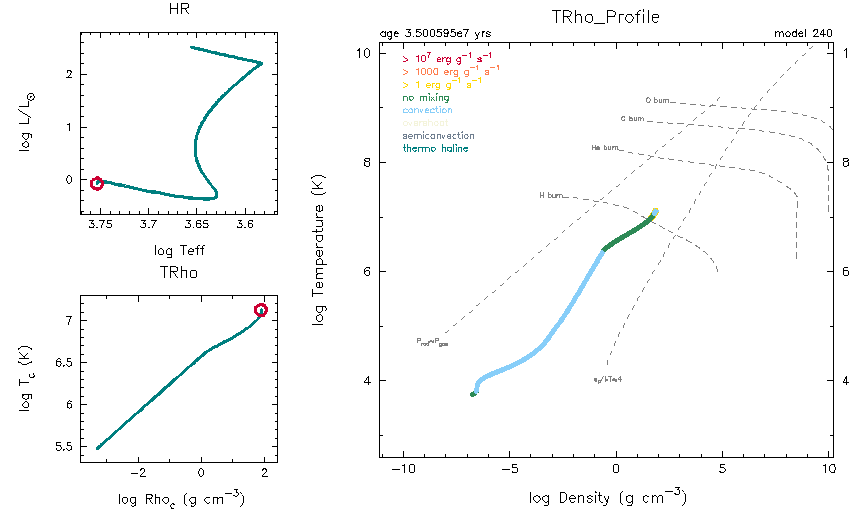
\includegraphics[width=0.9\textwidth]{Grid1_00240}
\caption{Graphical output from a \mesa\ run of a $\val{1}{\Msun}$ PMS star. \label{f.mesa-fig}}
\end{figure}

The large plot labeled `|TRho_profile|' shows the run of temperature $T$ versus density $\rho$ in the star, with the various colors indicating mixing and energy generating regions. The small plot labeled `|HR|' traces the history of luminosity $L$, in units of the solar luminosity $\Lsun$, versus effective temperature $\Teff$. The other small plot labeled `|TRho|' traces the history of the central temperature $T_{c}$ versus the central density $\rho_{c}$.

\begin{exercisebox}[Contraction of a star to the main sequence]
\begin{enumerate}
\item How long did the star take to contract to the main sequence?
\item What are $L$, $\Teff$, $T_{c}$, and $\rho_{c}$ when the star begins H burning?
\item Describe how the fraction of the star that is convective changes during the run.
\end{enumerate}
\end{exercisebox}

\subsection{A peak under the hood}
To understand what just happened, we start with the command `|./rn|'. This is just a script---you can open it with a text editor---containing the following.
\VerbatimInput{introduction/1M-pms/rn}
This just gets some information about the version of \mesa\ being used (the `|svn info|' directive), removes any pre-existing file with restart information, prints the date, runs star, and then prints the date again.

The command `|star|' is built from the source code in `|src/run.f|'. This is a very short program.  The relevant lines
\VerbatimInput[firstline=11,lastline=16]{introduction/1M-pms/src/run.f}
direct the program to read in parameters from a file `|inlist|' and then hand control to a subroutine, `|do_run_star|', within the \mesa\ library.

The file `|inlist|', is divided into three sections (each section begins with an `|&|' followed by the section name and ends with a `|/|'): `|star_job|', `|controls|', and `|pgstar|'.  The bang `|!|' denotes the start of a comment. This list is rather simple. The first section
\VerbatimInput[firstline=1,lastline=9]{introduction/1M-pms/inlist}
tells \mesa\ to read another file, `|1M_pms.inlist|'. The second section, `|&controls|' also tells \mesa\ to read in `|1M_pms.inlist|'. It is in `|1M_pms.inlist|' that all of the settings are placed, so take a quick peek at that file.  For example, in section `|&star_job|' the lines
\VerbatimInput[firstline=21,lastline=22]{introduction/1M-pms/1M_pms.inlist}
tell \mesa\ to pause and wait for the user to hit `|return|' before ending the code, and to activate the plotting windows. In section `|&controls|' the lines
\VerbatimInput[firstline=31,lastline=32]{introduction/1M-pms/1M_pms.inlist}
tell \mesa\ the initial mass and metallicity of the star, while the lines
\VerbatimInput[firstline=42,lastline=43]{introduction/1M-pms/1M_pms.inlist}
tell \mesa\ to stop when the total power from nuclear burning, $L_{\mathrm{nuc}}$, exceeds $0.95 L$, where $L$ is the total surface luminosity.

The third section of `|inlist|'
\VerbatimInput[firstline=18,lastline=26]{introduction/1M-pms/inlist}
reads in the parameters for the plot from `|basic_plot.inlist|'. There is another parameter file, `|track_scaled_vars.inlist|', but the flag to read that file is 
`|read_extra_pgstar_inlist2 = .false.|'  As you might guess, you'll be using this later on in the assignment.

\begin{center}
\fbox{\parbox{0.96\textwidth}{\textbf{Question:} There is a reason for nesting the parameter inlist files. Can you discern what that reason is?}}
\end{center}

Now that you've seen how the code in action, we are going to look a bit more at the architecture of \mesa. If you do `|ls $MESA_DIR|', you will see that \mesa\ is divided into modules: `|eos|' computes the equation of state, `|kap|' computes the opacity, and so forth. Within each module are two folders, `|public|' and `|private|'.  The `|public|' folder contains the interface of that module. The source file ending with `|_def.f|' contains the data structures used by that module, and the source file ending with `|_lib.f|' contains the routines for that module. The |private| directory contains the inner machinery of the module.

All of these modules can be used by themselves; the `|star|' module puts everything together to simulate stellar evolution. What |star| does is to evolve a stellar model---a complete description of a star at a given instant of time---forward in time by some amount $\Delta t$. String together a sequence of such models and you have a representation of the star's evolution. These models are not evenly spaced in time; rather, \mesa\ adjusts $\Delta t$ to keep the models accurate within specified tolerances. The |star| module contains, in addition to the |public| interface and |private| machinery, additional routines in the folder |job| for starting a run from some initial model and stopping that run when a specified condition is met.

\subsection{A MESA project}

The \mesa\ code that you installed is a library, a collection of routines that when combined simulate the evolution of a stellar-like object. To put everything together, you create a directory, such as `|1M-pms|'.  A template for such a directory is contained in `|$MESA_DIR/star/work|'---consult the `|README|' file there for instructions. 

The working directory is organized into several sub-directories. The `|make|' folder contains the `|makefile|' script for compiling the code. The `|src|' folder contains, in addition to the top-level `|run.f|' code, a collection of customizable routines in the file `|run_star_extras.f|'. In addition to these folders, the working directory contains a set of inlist files; these, as mentioned above, contain all of the parameters necessary to control the \mesa\ run and its output.  The complete listings of parameters and their default settings are contained in the directory `|$MESA_DIR/star/defaults|' in the three files `|*.defaults|'. The inlists in the work directory only need to contain those parameters that differ from the defaults.

The final components of the working directory are sub-directories to hold the output of \mesa.  The names of these are customizable and can be set in the inlists; by default, the main two are called `|LOGS|' and `|photos|'.  Within `|LOGS|' are the file `|history.data|' and the files `|profile|\textit{dd}|.data|'. The `|history.data|' file contains the time evolution of global stellar properties, such as luminosity, radius, surface effective temperature, and so on. The `|profile|\textit{dd}|.data|' files contain ``snapshots'' of the star's structure: the run of temperature, density, pressure, and so on with location within the star. 

\subsection{Exercise: customizing MESA output}

After that brief overview of the \mesa\ architecture, let's do something concrete: we'll customize \mesa\ to have it generate a plot of a variable that we define.  In this chapter, we've argued that the central pressure of a star should scale as $P_{c}\propto GM^{2}/R^{4}$. We also found that the central density should scale as the mean density, $\rho_{c}\propto \bar{\rho} = 3M/(4\pi R^{3})$. Exercise~\ref{ex.central-temperature} asks you to find the central temperature in terms of $M$, $R$, and mean molecular weight $\mu$. What the derivation in the chapter doesn't tell us is the coefficient $\rho_{c}/\bar{\rho}$ and its counterparts for pressure and temperature.  We can use \mesa, however, to test these scalings and extract these constants of proportionality.

To do this, we modify the code in `|src/run_star_extras.f|'.  What we want is for \mesa\ to calculate $P_{\mathrm{scale}} = GM^{2}/R^{4}$, $\rho_{\mathrm{scale}} = \bar{\rho}$, and $T_{\mathrm{scale}}$, and then write out the values of $P_{c}/P_{\mathrm{scale}}$, $\rho_{c}/\rho_{\mathrm{scale}}$, and $T_{c}/T_{\mathrm{scale}}$ in the file `|history.data|'. To do this, we first tell \mesa\ how many extra columns in `|history.data|' we need:
\VerbatimInput[firstline=96,lastline=104,gobble=8]{introduction/1M-pms/src/run_star_extras.f}
Here I am adding one column, which will be $P_{c}/P_{\mathrm{scale}}$.  When you implement the other scalings, you'll change the variable \verb|how_many_extra_history_columns| to reflect that we need three columns.

Next, we need to compute the data for these columns.  We therefore modify the following routine.
\VerbatimInput[firstline=107,lastline=154,gobble=8]{introduction/1M-pms/src/run_star_extras.f}
In detail, we first declare the extra variables we need.
\VerbatimInput[firstline=113,lastline=113,gobble=8]{introduction/1M-pms/src/run_star_extras.f}
Next, we give each column a name.
\VerbatimInput[firstline=124,lastline=126,gobble=8]{introduction/1M-pms/src/run_star_extras.f}
Notice that the latter two are commented out (`|!|'); for this example; you'll need to uncomment them to print out the other variables.

We are then ready to compute our values.  Note that \mesa\ defines many physical constants in `|$MESA_DIR/const/public/const_def.f|'; we therefore use this in line 130 for $G$, and you can read the hint in lines 143ff. Next, we need to get the values of $M$, $R$, $\mu_{c}$, $P_{c}$, $\rho_{c}$, and $T_{c}$. These are provided in a data structure |s|, which the routine fetches
\VerbatimInput[firstline=116,lastline=116,gobble=8]{introduction/1M-pms/src/run_star_extras.f}
from the variable |id| that is passed to the routine.  To see a complete list of what is in this data structure, look at `|$MESA_DIR/star/public/star_data.inc|'. I've already taken care of computing $M$, $R$, $\mu_{c}$, and $P_{\mathrm{scale}}$ for you.  The values of our scaled variables are then stored in the array `|vals|'; you will fill in the second and third members of the array.

If you look in `|LOGS/history.data|', you should see that the last column is indeed `|Pc_scaled|', as expected. Of course, we'd like to display it graphically, and \mesa\ does predefine plots that can display values in `|history.data|'. We customized the output in `|track_scaled_vars.inlist|':
\VerbatimInput{introduction/1M-pms/track_scaled_vars.inlist}
To use this, we activate the window by setting the flag in line 3 to `|.true.|'. If we want to save our output, we set the `|file_flag = .true.|' in line 11.  

\UndefineShortVerb{\|}


% !TEX root = ./notes.tex
\chapter[Stellar Structure Equations]{The Lagrangian Equations of Stellar Structure}

After exploring the polytropic models, we are now ready to write the general equations for stellar structure in one-dimension. We will start from our equations derived in \S~\ref{s.fluid-introduction}, namely continuity (conservation of mass)
\begin{equation}\label{e.mass-1}
\partial_{t}\rho + \divr(\rho\vu) = 0,
\end{equation}
and the Euler equation,
\begin{equation}\label{e.momentum-1}
\partial_{t}\vu + \vu\cdot\grad\vu = -\grad \Phi - \frac{1}{\rho}\grad P.
\end{equation}
Note that if we multiply eq.~(\ref{e.momentum-1}) by $\rho$, we can rewrite it, using eq.~(\ref{e.mass-1}), as
\begin{equation}\label{e.momentum-2}
	\partial_{t}(\rho\vu) + \divr[\vu(\rho\vu)] = -\rho\grad\Phi -\grad P.
\end{equation}
The left-hand side is interpreted as expressing the conservation of momentum ($\rho\vu$) in the absence of forces, analogous to eq.~(\ref{e.mass-1}) for the conservation of mass ($\rho$).

The next equation is that of energy conservation. Here we must consider both the internal energy per unit volume $E/V = \rho e$ and the kinetic energy per unit volume $\rho u^{2}/2$.  In this section $e$ represents the internal energy per unit mass of the fluid. In a fixed volume of the fluid the total energy is then 
\[ \int_{V}(\rho \frac{1}{2}u^{2} + \rho e)\,\dif V. \]
The flux of energy into this volume will clearly include
\[ -\int_{V}\left(\frac{1}{2}\rho u^{2} + \rho e\right) \vu\vdot\dif\bvec{S}. \]
But wait, there's more!  In addition, we have a conductive heat flux, 
\[-\int_{\partial V}\bvec{F}\vdot\dif\bvec{S}.\] 
Moreover, the pressure acting on fluid flowing into our volume does work on the gas at a rate 
\[-\int_{\partial V}P\vu\vdot\dif\bvec{S}.\] 
As a result, the net change of energy in our volume is 
\begin{equation}\label{e.energy-1}
\partial_{t}\int_{V}\left(\frac{1}{2}\rho u^{2} + \rho e\right)\nsp\dif V 
	= -\int_{\partial V} \!\dif\bvec{S}\vdot\left[\vu\left(\frac{1}{2}\rho u^{2} + \rho e + P\right) + \bvec{F}\right].
\end{equation}
Expressed in differential form, this is
\begin{equation}\label{e.energy-2}
 \partial_{t}\left(\frac{1}{2}\rho u^{2} + \rho e\right) 
 	+ \divr\left[\rho\vu\left(\frac{1}{2} u^{2} + e + \frac{P}{\rho}\right)\right]
	+ \divr\bvec{F} = \rho\varepsilon + \rho \vu\vdot\bvec{g}.
\end{equation}
We've added the right-hand side to account for ssource, such as nuclear reactions or sinks, such as neutrino losses of energy, and I've added a work term due to gravity.
You are probably wondering at this point why I didn't put gravity, which can be expressed as a potential, on the left hand side of this equation.  The reason is that the gravitation stresses cannot be expressed in a  \emph{locally} conservative form; it is only when integrating over all space that the conservation law appears.

The heat flux $\bvec{F}$ is related, in the diffusion approximation, to the gradient of temperature,
\begin{equation}\label{e.flux-1}
\bvec{F} = -\frac{4}{3}\frac{acT^{3}}{\rho\kappa}\grad T.
\end{equation}
Equations~(\ref{e.mass-1}), (\ref{e.momentum-2}), (\ref{e.energy-2}), and (\ref{e.flux-1}), along with an equation of state $P = P(\rho,t)$, form our basic equations for the structure of the star.  They are not, however, in the most useful form, however; the stellar radius is not fixed, but for may stars the mass is very nearly constant over much of the star's life.  

It is more useful to transform these coordinates from $(r,t)$ to $(m,t)$, where $m$ is the mass within a sphere of radius $r$.  Appendix~\ref{s.lagrangian-appendix} contains a description of the mathematics; in short, the transformation consists of making the change
\begin{eqnarray}
	\label{e.lagrange-rule-1}
	\left.\frac{\partial}{\partial_{t}}\right|_{r} + u\left.\frac{\partial}{\partial r}\right|_{t} 
	&\to& \left.\frac{\partial}{\partial t}\right|_{m} \equiv \frac{\Dif}{\Dif t} \\
	\label{e.lagrange-rule-2}
	\left.\frac{\partial}{\partial r}\right|_{t} &\to& 4\pi r^{2}\rho \left.\frac{\partial}{\partial m}\right|_{t}.
\end{eqnarray}
In deriving this change, we used the equation of continuity, which becomes
\begin{equation}\label{e.lagrange-r}
\frac{\partial r}{\partial m} = \frac{1}{4\pi r^{2}\rho}.
\end{equation}
Our equation for momentum (eq.~[\ref{e.momentum-1}]) becomes
\begin{equation}\label{e.lagrange-momentum}
\frac{\partial P}{\partial m} = -\frac{Gm}{4\pi r^{4}} - \frac{1}{4\pi r^{2}}\frac{\partial u}{\partial t}.
\end{equation}
In hydrostatic balance the second term on the right-hand side is negligible.  We stress that here $\partial/\partial t$ is now taken at fixed $m$, and thus it follows a fixed fluid element.  The flux equation, (eq.~[\ref{e.flux-1}]) can be transformed to
\begin{equation}\label{e.lagrange-flux}
	\frac{\partial T}{\partial m} = -\frac{3}{64\pi^{2}r^{4}}\frac{\kappa}{ac T^{3}}L_{r}.
\end{equation}
Here $L_{r}$ is the luminous flux at a radius $r$. 

The energy equation (eq.~[\ref{e.energy-2}]) is more complicated. We can expand the time derivative as
\begin{eqnarray*}
	\partial_{t}(\frac{1}{2}\rho u^{2} + \rho e) 
	&=& \left(\frac{1}{2}u^{2} + e\right)\partial_{t}\rho + \rho\partial_{t}\left[\frac{1}{2}(\vu\vdot\vu) + e\right]\\
	&=& -\left(\frac{1}{2}u^{2} + e\right)\divr\left(\rho\vu\right) + \rho \vu\partial_{t}\vu + \rho\partial_{t}e,
\end{eqnarray*}
using equation~(\ref{e.mass-1}) to substitute for $\partial_{t}\rho$.  We then use equation~(\ref{e.momentum-1}) to replace $\partial_{t}\vu$, and recognizing that $\vu(\vu\vdot\grad)\vu = \vu\vdot\grad[(1/2)u^{2}]$, rewrite equation~(\ref{e.energy-2}) as
\[ 
	\rho\left(\partial_{t} + \vu\vdot\grad\right) e + P\divr\vu = -\divr\bvec{F} + \rho\varepsilon.
\]
We've canceled all common factors here.  Finally, we once again use equation~(\ref{e.mass-1}) to set 
\[
	P\divr\vu = -(P/\rho)(\partial_{t}\rho + \vu\vdot\grad \rho) 
	= \rho P\left(\partial_{t} + \vu\vdot\grad\right)\left(\frac{1}{\rho}\right).
\]
Now we have the left side in terms of the Lagrangian time derivative $\Dif/\Dif t$.  Note that when we combine terms, the left-hand side contains 
\[ \Dif e/\Dif t + P\Dif (1/\rho)/\Dif t = T\Dif s/\Dif t \] 
where the equality follows from the first law of thermodynamics.

For the right-hand side, we expand the divergence operator in spherical symmetry and use equation~(\ref{e.lagrange-rule-2}) to obtain
\[
	-\divr\bvec{F} = -\frac{1}{r^{2}}\frac{\partial(r^{2} F)}{\partial r} = -\rho\frac{\partial L_{r}}{\partial m}.
\]
Putting everything together, we finally have our Lagrangian heat equation,
\begin{equation}\label{e.lagrange-heat}
	\frac{\partial L_{r}}{\partial m} = \varepsilon - T\frac{\Dif s}{\Dif t}.
\end{equation}
This has a simple interpretation: the change in luminosity across a mass shell is due to sources or sinks of energy and the change in the heat content of the shell.  It is more useful, however, to work with temperature and pressure, for which we already have expressed via equations~(\ref{e.lagrange-momentum}) and (\ref{e.flux-1}).  Write
\[
	T\frac{\Dif s}{\Dif t} = T\tderiv{s}{T}{P}\frac{\Dif T}{\Dif t} + T\tderiv{s}{P}{T}\frac{\Dif P}{\Dif t},
\]
and use the identity (see Appendix~\ref{s.thermo-derivatives})
\[
	\tderiv{s}{P}{T} = -\tderiv{s}{T}{P}\tderiv{T}{P}{s}
\]
to obtain
\begin{equation}\label{e.lagrange-heat-alt}
	\frac{\partial L_{r}}{\partial m} 
	= \varepsilon - c_{P}\left[ \frac{\Dif T}{\Dif t} - \tderiv{T}{P}{s} \frac{\Dif P}{\Dif t}\right].
\end{equation}
Equations~(\ref{e.lagrange-r}), (\ref{e.lagrange-momentum}), (\ref{e.lagrange-flux}), and (\ref{e.lagrange-heat-alt}), when supplemented by an equation of state, a Rosseland mean opacity, and the equations for nuclear heating and neutrino cooling, are the equations for stellar structure and evolution in spherical symmetry. We must also include a treatment of the photosphere (chapter~\ref{s.stellar-atmospheres}) and a phenomenological treatment of convection as well.

% !TEX root = ./stellar-notes.tex
\chapter{Convection}\label{s.convection}

Hot air rises, as a glider pilot or hawk can tell you. The fluid velocities in question are very subsonic, so we have hydrostatic equilibrium to excellent approximation. But the fluid motions make an enormous difference for heat transport! This state of fluid motions induced by a temperature gradient is known as \emph{convection}. You can perform the following demonstration of the onset of convection.  Brew tea, and pour the hot tea into a saucepan that is on an unlit burner.  Use a straw with your thumb over the top to insert a layer of cold milk under the warm tea in the saucepan.  The temperature difference between the tea and milk will inhibit their mixing. Light the burner, and watch for the development of convection---you will know it when you see it.

\begin{figure}[htbp]
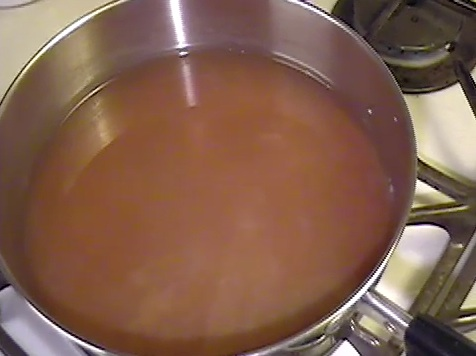
\includegraphics[width=0.5\linewidth]{convection-1}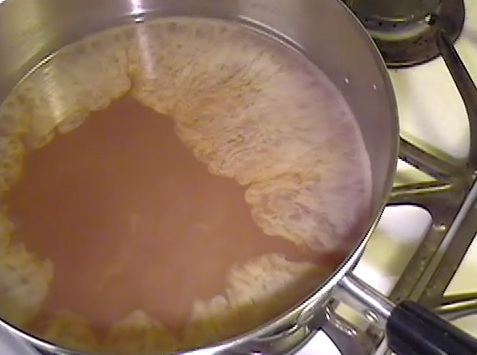
\includegraphics[width=0.5\linewidth]{convection-2}
\caption{Onset of convection in a tea-milk mixture.\label{f.tea}}
\end{figure}

\section{Criteria for onset of convection}\label{s.convection-onset}

To understand this process, let's consider a fluid in planar geometry and hydrostatic equilibrium,
\begin{equation}
\frac{\dif P}{\dif r} = -\rho g.
\end{equation}
Now, imagine moving a blob of fluid upwards from $r$ to $r+h$.  We move the blob slowly enough that it is in hydrostatic equilibrium with its new surroundings, $P_{b}(r+h) = P(r+h)$, where the subscript $b$ refers to ``blob.'' We do move the blob quickly enough, however,  that it does not remain in \emph{thermal} equilibrium with its surroundings; that is, we move the blob \emph{adiabatically}.  The entropy of the blob is therefore constant, 
$S_{b}(r+h) = S_{b}(r) = S(r)$, and is therefore not, in general, equal to the entropy of the surrounding gas at $r+h$: $S_{b}(r+h)  \neq S(r+h)$.  

As the blob rises, it displaces some of the surrounding fluid. Archimedes tells us that if the displaced fluid is less massive than the blob, then the blob will sink.  We can rephrase this in terms of the volume occupied by a unit mass of fluid $V$: if the volume occupied by the blob is less than the volume of an equal mass of background, then the blob will sink. Translating this into an equation: if
\begin{eqnarray}
\lefteqn{V[P(r+h),S(r+h)] - V_{b}[P_{b}(r+h),S_{b}(r+h)] =}\nonumber\\
&&  V[P(r+h),S(r+h)] - V[P(r+h),S(r)] > 0
\label{e.archimedes}
\end{eqnarray}
then the blob will sink. If condition (\ref{e.archimedes}) is violated, the blob will continue to rise, and the system is unstable to convection.  
Figure~\ref{f.convective-schematic} has a cartoon of this process.

\begin{marginfigure}
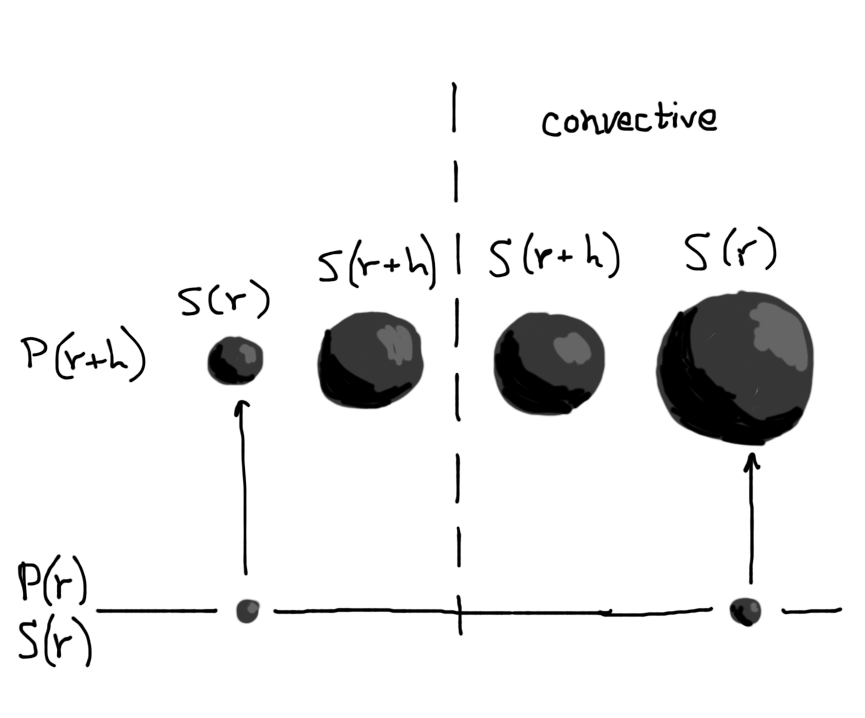
\includegraphics[width=\textwidth]{convective}
\caption[Illustration of criteria for convective instability.]{\label{f.convective-schematic}Illustration of criteria for convective instability.  On the left, raising a blob a distance $h$ adiabatically and in pressure balance with its surrounding results in a higher density $V_{b} < V$.  This is stable: the blob will sink back.  On the right, the blob is less dense and hence buoyant: it will continue to rise.}
\end{marginfigure}

Taking $h$ to be an infinitesimal displacement and expanding the left-hand side of equation~(\ref{e.archimedes}) gives us a local condition for stability:
\begin{equation}\label{e.convective-stability}
V[P(r+h),S(r)] + \tderiv{V}{S}{P}\frac{\dif S}{\dif r} - V[P(r+h),S(r)]  = \tderiv{V}{S}{P}\frac{\dif S}{\dif r} > 0 .
\end{equation}
Noting that
\begin{eqnarray*}
\tderiv{V}{T}{P} &=& \tderiv{V}{S}{P}\tderiv{S}{T}{P}\\
 &=& \frac{C_{P}}{T}\tderiv{V}{S}{P},
 \end{eqnarray*}
 we can rewrite equation~(\ref{e.convective-stability}) as
 \[
 \frac{T}{C_{P}}\tderiv{V}{T}{P}\frac{\dif S}{\dif r} > 0.
 \]
Now, $(\partial V/\partial T)_{P}$ is positive (gas expands on being heated), so our condition for stability is simply
 \begin{equation}\label{e.entropy-condition}
\frac{\dif S}{\dif r} > 0.
\end{equation}
In a convectively stable star, the entropy must increase with radius. if $\dif S/\dif r < 0$, then convection occurs and carries high-entropy material outward, where it will eventually mix with the ambient medium.  As a result, convection drives the entropy gradient toward the marginally stable configuration $\dif S/\dif r = 0$.  If a star is fully convective and mixes efficiently, then the interior of the star lies along an adiabat. 

\newpage
\begin{exercisebox}
Assuming that $\nabla \approx \nablaad$ in a convective region, sketch a plot of temperature as a function of pressure for the following cases.
\begin{enumerate}
\item A star with a stable inner layer and a convective outer layer;
\item A star with a convective inner layer and and a stable outer layer.
\end{enumerate}
Indicate on both of these plots an adiabat.
\end{exercisebox}

\newthought{We can derive a condition for convective stability} in terms of the local gradients of temperature and pressure. Writing $S = S[P(r),T(r)]$ we expand equation~(\ref{e.entropy-condition}) to obtain
\begin{equation}\label{e.schwarzschild-1}
\frac{\dif S}{\dif r} = \tderiv{S}{P}{T} \frac{\dif P}{\dif r} + \tderiv{S}{T}{P}\frac{\dif T}{\dif r} .
\end{equation}
Now, $P$ is a monotonically decreasing function of $r$, which means we can use it as a spatial coordinate and write,
\begin{equation}\label{e.TPstar}
\frac{\dif T}{\dif r} = \TPstar \frac{\dif P}{\dif r} .
\end{equation}
Here $\dif T/\dif P|_{\star}$ is the slope of the $T(P)$ relation \emph{for the stellar interior}.  In particular, this is \emph{not} a thermodynamic equality. Substituting equation~(\ref{e.TPstar}) into equation~(\ref{e.schwarzschild-1}), using hydrostatic equilibrium to eliminate $\dif P/\dif r$, and recognizing that $(\partial S/\partial T)_{P} = C_{P}/T$, we obtain
\begin{equation}\label{e.schwarzschild-2}
\frac{\dif S}{\dif r} =  -\rho g\left[\tderiv{S}{P}{T} + \frac{C_{P}}{T} \TPstar \right].
\end{equation}
Finally, we can use the identity (see Appendix~\ref{s.thermo-derivatives})
\begin{equation}
\tderiv{S}{P}{T}\tderiv{T}{S}{P}\tderiv{P}{T}{S} = -1
\end{equation}
to simplify equation~(\ref{e.schwarzschild-2}),
\begin{eqnarray}
\frac{\dif S}{\dif r} &=& -\frac{\rho g}{P}C_{P}\left[\frac{P}{T}\TPstar - \frac{P}{T}\tderiv{T}{P}{S}\right]\nonumber \\
 & = & -\frac{\rho g}{P}C_{P}\left[\nabla - \nablaad\right].
 \label{e.schwarzschild}
\end{eqnarray}
Here we have introduced the shorthand notation $\nabla\equiv \dif \ln T/\dif\ln P|_{\star}$ and $\nablaad \equiv \left(\partial \ln T/\partial\ln P\right)_{S}$.
\emph{A mixture of uniform composition is unstable to convection if the local temperature gradient is steeper than an adiabat, i.e., if $\nabla > \nablaad$.}

\section{A second look at convective instability}\label{s.convection-second-look}

Here we'll take a second-look at the convection by imagining we have a background state with $\vu=0$; we then \emph{perturb} state by displacing fluid elements a distance $\delta\vr$, and obtaining an equation of motion for $\delta\ddot{\vr}$.  This requires a bit of careful thought on what we are perturbing.

\begin{marginfigure}[18\baselineskip]
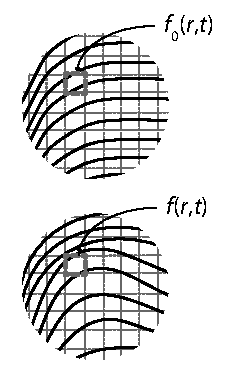
\includegraphics[width=\linewidth]{eulerian}
\caption{\label{f.eulerian-grid-1} An Eulerian perturbation: we compare fluid quantities at corresponding locations.}
\end{marginfigure}
There are two types of perturbations. We may change a fluid quantity $f$ at a fixed location $\vr$ and time $t$ (Fig.~\ref{f.eulerian-grid-1}):
\begin{equation}\label{e.eulerian-perturbation}
  \Delta f \equiv f(\vr,t)-f_{0}(\vr,t),
\end{equation}
where the subscript ``0'' denotes the unperturbed quantity.  We call $\Delta f$ an \emph{Eulerian perturbation}.  

We may also change a fluid quantity $f$ for a given fluid element; the position of this fluid element in the perturbed system is not necessarily at the same position as in the unperturbed case, however (Fig.~\ref{f.lagrangian-grid-1}):
\begin{equation}\label{e.lagrangian-perturbation}
 \delta f \equiv f(\vr,t) - f_{0}(\vr_{0},t).
\end{equation}
We call $\delta f$ a \emph{Lagrangian perturbation}. 
\begin{marginfigure}[280pt]
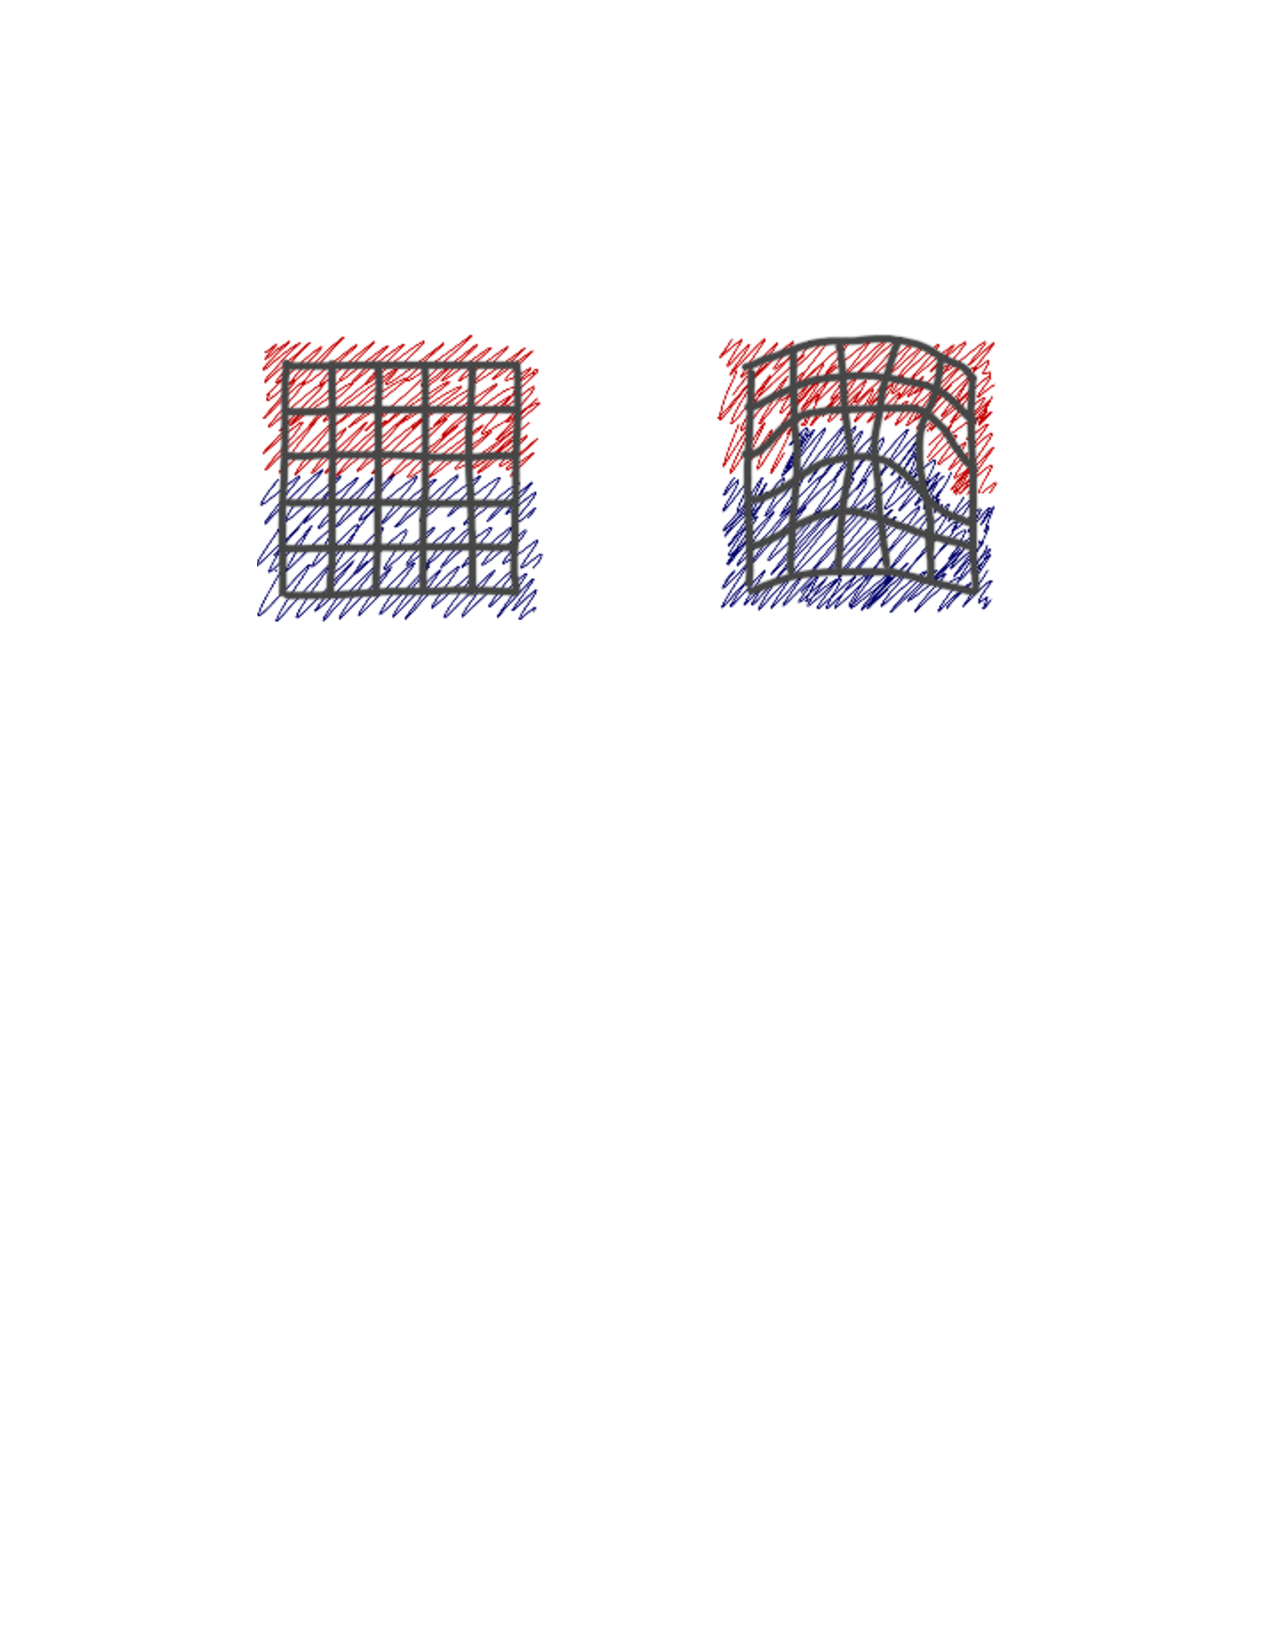
\includegraphics[width=\linewidth]{lagrangian}
\caption{\label{f.lagrangian-grid-1} A Lagrangian perturbation: we compare fluid quantities for corresponding fluid elements.}
\end{marginfigure}

Since the fluid element is displaced $\delta\vr = \vr-\vr_{0}$, we can add and subtract $f_{0}(\vr,t)$ to eq.~(\ref{e.lagrangian-perturbation}) and expand $f_{0}(\vr,t)$ to first order in $\delta \vr$ to obtain a relation between the two types of perturbations:
\begin{equation}\label{e.perturbation-relation}
\delta f = \Delta f + (\delta\vr\vdot\grad)f_{0}.
\end{equation}
There are a few useful commutation relations that are easily proved:
\begin{eqnarray}
\partial_{t}\Delta f &=& \Delta\left(\partial_{t}f\right),\\
\grad \Delta f &=& \Delta \grad f,\\
\frac{\Dif}{\Dif t}\delta f &=& \delta \frac{\Dif f}{\Dif t}.
\end{eqnarray}
And there are operations that do not commute:
\begin{eqnarray}
\partial_{t}\delta f &\neq& \delta\left(\partial_{t}f\right),\\
\grad \delta f &\neq& \delta \grad f,\\
\frac{\Dif}{\Dif t}\Delta f &\neq& \Delta \frac{\Dif f}{\Dif t}.
\end{eqnarray}
One can further show that $\delta\vu = (\Dif/\Dif t)\delta \vr$. Finally if the fluid has unperturbed velocity $\vu = 0$, then $\Delta \vu = \delta \vu$.

\newthought{Armed with these relations, let us perturb the momentum equation} by adiabatically displacing a fluid element a distance $\delta\vr$.  We will do this in such a way that the pressure at a fixed location does not change, i.e., $\Delta P = 0$. Of course, the pressure and density of a given fluid element will change according to the relation
\[
\frac{\delta P}{P} = \Gamma_{1}\frac{\delta\rho}{\rho}.
\]
We'll also assume that the gravitational force does not change, $\Delta g = 0$.  Our perturbed momentum equation then becomes
\[
\frac{\Dif^{2}\delta\vr}{\Dif t^{2}} = -\frac{1}{\rho + \Delta \rho}\grad P+ \bvec{g}.
\]
Since in the unperturbed fluid $\grad P = \rho\bvec{g}$, this equation simplifies to
\begin{equation}\label{e.perturbed-momentum}
\frac{\Dif^{2}\delta\vr}{\Dif t^{2}} = \frac{\Delta \rho}{\rho}\bvec{g}.
\end{equation}
Expanding,
\begin{eqnarray*}
\frac{\Delta \rho}{\rho} &=& \frac{\delta \rho}{\rho} - \frac{1}{\rho}(\delta\vr\vdot\grad)\rho = \frac{1}{\Gamma_{1}}\frac{\delta P}{P} - \frac{1}{\rho}(\delta\vr\vdot\grad)\rho\\
 &=& \frac{1}{\Gamma_{1}}\frac{\Delta P}{P} + (\delta\vr\vdot\grad)\left[\frac{1}{\Gamma_{1}}\ln P-\ln \rho\right].
\end{eqnarray*}
Since by assumption $\Delta P = 0$, the radial component of equation (\ref{e.perturbed-momentum}) becomes
\begin{equation}\label{e.blob-eq-of-motion}
\delta\ddot{\vr} = g\left[ \frac{\dif\ln\rho}{\dif r} - \frac{1}{\Gamma_{1}}\frac{\dif\ln P}{\dif r} \right] \,\delta r 
	\equiv g \mathcal{A} \delta r.
\end{equation}
The quantity $\mathcal{A}$ is called the \emph{Schwarzschild discriminant}: if $\mathcal{A} < 0$, then the motion is oscillatory with frequency $N = (-g\mathcal{A})^{1/2}$; $N$ is called the \emph{Brunt-V\"ais\"al\"a} frequency. The condition $\mathcal{A} > 0$ implies that the fluid is convectively unstable; and indeed, one can show that $\mathcal{A} > 0$ is equivalent to $\dif S/\dif r < 0$.

\section{Efficiency of Heat Transport}

A superadiabatic temperature gradient, $\nabla > \nablaad$, induces convective motions. A rising blob will be hotter than its surroundings and heat will therefore be conducted from the blob to its surroundings as it rises. The efficiency by which the heat is transported determines by how much convection is able to drive the temperature gradient towards an adiabat. Clearly the gradient must be super-adiabatic to drive the convection in the first place. We shall see, however, that in stars the difference between the gradient and the adiabat are typically exceedingly small. In other words, convection is extraordinarily efficient at transporting heat.

To understand this, let's go back to equation~\ref{e.perturbed-momentum}.  Write $\Delta\rho$ as stemming from differences in temperature between rising and falling blobs (recall that $\Delta P=0$).   With this substitution, we have
\begin{equation}\label{e.perturbed-navier-stokes}
 (\partial_{t}\vu + \vu\vdot\grad\vu) = \frac{\Delta\rho}{\rho}\vg = \left(\frac{\partial\ln\rho}{\partial\ln T}\right)_{P}\frac{\Delta T}{T}\vg.
 \end{equation}
%Heat conduction follows the equation
%\begin{equation}\label{e.heat-conduction}
%\rho C_{p}(\partial_{t} + \vu\cdot\grad)T = -\divr \bvec{F} = K\nabla^{2} T
%\end{equation}
%where $K$ is the effective thermal conductivity (includes contributions from both radiative and electronic transport of heat).
Our goal is to estimate the velocity of convective motions $u$, the departure of the temperature gradient from an adiabat $\Delta T$, and the fraction of the total heat flux carried by convective motions from these equations.

First, the velocity.  The left-hand side of equation~(\ref{e.perturbed-navier-stokes}) has a characteristic scale $\sim U^{2}/L$, whereas the right-hand side has a scale $g\Delta T/T$. (Recall that in an ideal gas, $(\partial\ln \rho/\partial\ln T)_{P} = -1$.)  If we take $L \sim c_{s}^{2}/g$, a pressure scale height, than we get an estimate of the convective velocity,
\begin{equation}\label{e.convective-velocity-estimate}
\frac{U}{c_{s}} \sim \left(\frac{\Delta T}{T}\right)^{1/2}.
\end{equation}
What is the heat flux carried by convection? Hot fluid rises and carries an excess of heat, per gram, of $c_{P}\Delta T$, giving a heat flux $\approx \rho \vu c_{P}\Delta T$. Thus to carry a given flux $F$, we have
\begin{equation}\label{e.convective-flux-estimate}
c_{s}\rho c_{P} T\left(\frac{\Delta T}{T}\right)^{3/2} \sim F.
\end{equation}
Note that in order of magnitude, $c_{P}T \sim c_{s}^{2}$, so 
\[
\frac{U}{c_{s}} \sim \left(\frac{\Delta T}{T}\right)^{1/2} \sim \left(\frac{F}{\rho c_{s}^{3}}\right)^{1/3}.
\]
For conditions in the solar interior, $F \ll \rho c_{s}^{3}$, and therefore the convective velocities are very subsonic. Indeed,
\begin{eqnarray*}
 \frac{F}{\rho c_{s}^{3}} &\sim& \frac{L_{\sun}}{4\pi \Rsun^{2}}\frac{4\pi \Rsun^{3}}{3\Msun}\left(\frac{\Rsun}{G\Msun}\right)^{3/2}\\
  &\sim& \frac{L_{\sun}}{G\Msun^{2}/\Rsun}\left(\frac{\Rsun^{3}}{G\Msun}\right)^{1/2} \\
 	&\sim& \frac{t_{\mathrm{dyn}}}{t_{\mathrm{KH}}} \ll 1.
\end{eqnarray*}
That is, the ratio of the solar flux to what could be carried for near-sonic convective motions is of the order of the dynamical timescale to the Kelvin-Helmholtz timescale.
We therefore expect that in a convective region, slow circulation will produce a temperature gradient that is very nearly adiabatic. This argument breaks down near the surface, where the cooling time of a fluid layer (the ``local'' Kelvin-Helmholtz timescale) can be small.

\section{Turbulence}
 
From the discussion of the previous section, it might seem possible, given the boundary conditions, of solving for the flow planform, that is, the velocity profile $\vu(\vx,t)$. This is decidedly not the case, however: the flow is turbulent, with intermittent velocity fluctuations seen over a large dynamical range of spatial and temporal scales. Modeling of such flows is a vexing problem in fluid dynamics.

To explore this topic a bit further, we need to introduce the concept of dynamical similarity.  Suppose you want to optimize a wing shape for an aircraft, and you wish to test its performance in a wind tunnel.  Why should you expect that the behavior of a model wing will have any relation to the full-scale one?  

To see how this works, start with the Navier-Stokes equation (for simplicity, we'll keep it in one dimension):
\begin{equation}\label{e.navier-stokes-with-visc}
	(\partial_{t} + u\cdot\partial_{x})u = -\frac{1}{\rho}\partial_{x}P + \nu \partial_{x}^{2}u.
\end{equation}
Here $\nu$ is the coefficient of kinematic viscosity, with dimensions $[\nu]\sim [\textrm{length}]^{2}\cdot [\textrm{time}]^{-1}$.
Let's recast equation~(\ref{e.navier-stokes-with-visc}) into dimensionless form by scaling our variable: let $L$ and $U$ represent the characteristic length and velocity scales, and define the dimensionless variables $\tilde{x} = x / L$ and $\tilde{u} = u / U$. This choice then implicitly defines the time variable, $\tilde{t} = t\cdot U/L$. Upon changing to the variables $\tilde{x}$, $\tilde{u}$, and $\tilde{t}$, and writing the equation of state as $P = c_{s}^{2} \rho$ (appropriate for adiabatic flow---we are ignoring heat conduction), we obtain the equation
\begin{equation}\label{e.scaled-NS}
	(\partial_{\tilde{t}} + \tilde{u}\cdot\partial_{\tilde{x}})\tilde{u} = -\left\{\frac{c_{s}^{2}}{U^{2}}\right\}\partial_{\tilde{x}}\ln\tilde{\rho} + \left\{\frac{\nu}{UL}\right\} \partial_{\tilde{x}}^{2}\tilde{u}.
\end{equation}
Each term in this equation is dimensionless.  The physical characteristics of the fluid and the scales involved are described by just two dimensionless parameters:
\begin{eqnarray*}
 \Ma\equiv\frac{U}{c_{s}}&\qquad& \textrm{Mach number (measure of compressibility)}\\
 \Rey\equiv \frac{UL}{\nu} &\qquad& \textrm{Reynolds number (measure of viscous forces)}
\end{eqnarray*}
So, if we build a model wing at a certain scale and place it in a wind tunnel with a certain velocity, then by adjusting the density and temperature (and hence the sound speed and viscosity) to the desired $\Ma$ and $\Rey$, the flow pattern in our model will faithfully replicate the flow in the actual system.

For stellar  convection, $\Ma\ll 1$. What about \Rey?  In typical astrophysical plasmas, the large lengthscales make \Rey\ ludicrously large. Terrestrial experiments and simulations cannot approach this regime. Experimentally, when $\Rey \gtrsim 10^{3}$, then flow becomes \emph{turbulent}: the velocity has strong intermittent fluctuations across a wide range of lengthscales and timescales.  How to characterize the flow in such a case? It is useful to describe the flow in terms of correlated velocities---an ``eddy''---which have some lengthscale.

Suppose we pass water through a pipe that has an embedded mesh screen (Fig.~\ref{f.turbulence}).  For sufficiently large $\Rey = UL/\nu$, where $L$ is the mesh spacing, the downstream flow becomes turbulent. The turbulent eddies are damped.  Now an eddy of size $\lambda$ has an effective Reynolds number $\Rey(\lambda) = U(\lambda)\lambda/\nu$; if this is very large, then molecular viscosity cannot be the reason for damping fluid motions on that scale. Instead what happens is that an eddy with lengthscale $\lambda$ and velocity scale $U(\lambda)$ drives eddies on a smaller scale $\lambda' < \lambda$. These in terms drive still smaller eddies, which in turn drive still smaller eddies, and so on, until eventually very tiny eddies are excited, with size $\lambda_{\nu} \sim \nu/U(\lambda_{\nu})$; and these eddies \emph{are} damped by viscosity!

\begin{marginfigure}
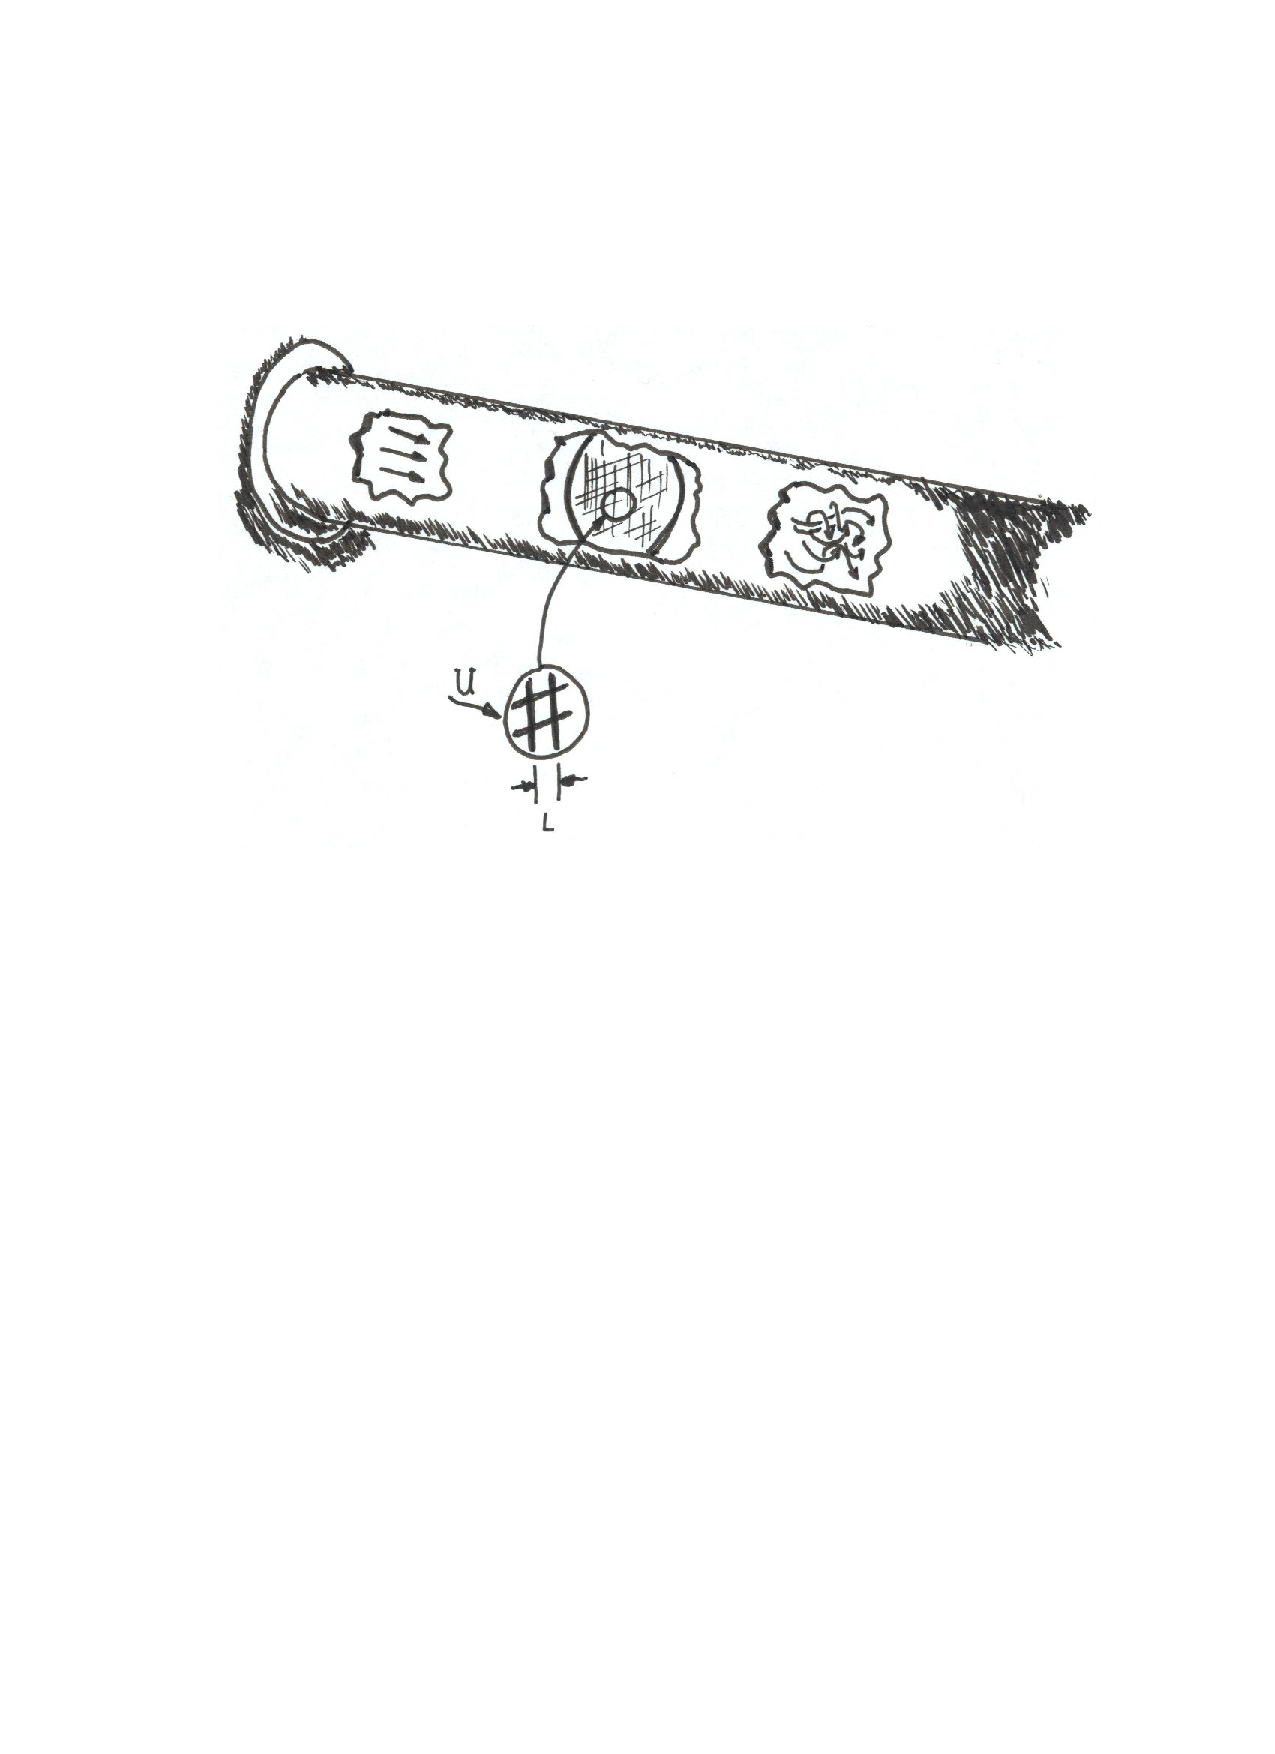
\includegraphics[width=\textwidth]{turbulence-maker}
\caption[A simple mechanism for generating turbulence.]{\label{f.turbulence} A simple mechanism for generating turbulence. A flow of water in a pipe (upstream velocity $U$) flows through a mesh (spacing $L$).  If $\Rey = UL/\nu$ is sufficiently large, the downstream flow becomes turbulent. }
\end{marginfigure}

Kolmogorov argued that in steady-state, intermediate-sized eddies (i.e., those with lengthscales $\nu/U(\lambda) \ll \lambda \ll L$) are neither losing or gaining energy and hence were transferring energy to smaller scales at the same rate as they were being driven; further, this rate at which energy is being transferred to smaller scales is just the net rate of dissipation in the fluid (which is done by the smallest eddies).  The huge dynamic range in lengthscales implies that the velocity of the eddy should not depend on either $L$ or $\nu$, and hence $U(\lambda)$ can only be a function of $\lambda$ (length) and the rate of energy dissipation per unit mass $\varepsilon$ ($\mathrm{energy/mass/time}\sim\mathrm{length^{2}/time^{3}}$). There is only one way to combine these quantities to form something with a dimension of length/time, and so
\begin{equation}\label{e.kolmogorov-velocity}
U(\lambda) \sim \varepsilon^{1/3}\lambda^{1/3}.
\end{equation}
This is seen experimentally: in flows with a large dynamic range of scales, the velocity spectrum follows a power-law with this slope, over an intermediate range of scales, the \emph{inertial range}.  A good example is the flow in a tidal channel\cite{Grant1962Turbulence-spec}.

% !TEX root = ./notes.tex
\chapter{Polytropes and the Lane-Emden Equation}

In the previous chapters, we derived the basic equations of stellar structure. To construct detailed models is clearly an involved task because there are many linked physical variables. For example, the equation of hydrostatic balance, eq.~(\ref{e.hydrostatic}), contains both $\rho$ and $P$; in order to connect these two variables we have to know the temperature, so in general we need in include an equation for heat transport and heat flux. Before diving into all that, however, we'll take a little digression to solve some simplified stellar models known as \textbf{polytropes}; these are useful not only for historical reasons, but they also allow for quick analytical calculations.

\section{Historical Background}\label{s.LE-background}

To understand where the term polytropic comes from, let's first consider an ideal gas in hydrostatic equilibrium, and furthermore suppose that the temperature and density lie along an adiabat.  In that case we have the following relations:
\begin{equation}\label{e.ideal-adiabatic-relations} 
T\rho^{1-\gamma} = \mathrm{const};\quad P\rho^{-\gamma} = \mathrm{const};\quad TP^{(1-\gamma)/\gamma} = \mathrm{const},
\end{equation}
which you will recall from elementary thermodynamics. Here $\gamma = C_{P}/C_{\rho}$ is the ratio of specific heats. The equation of state is
\begin{equation}\label{e.ideal-eos}
P = \left(\frac{\NA\kB}{\mu}\right)\rho T,
\end{equation}
where $\mu$ is the mean molecular weight and the quantity in parenthesis is $C_{P}-C_{\rho} = \NA\kB/\mu$.
We might imagine, for example, a rising plume of hot air in Earth's atmosphere.  There is one snag with this analysis for the troposphere, however: the condensation of water vapor means that one cannot hold $\dif s = 0$ in a rising plume of hot, moist air.  Attempting to model this moist convection in the Earth's troposphere motivated work in the early 1900's by Kelvin, Lane, Emden, and others to consider a more general problem, in which $T\dif s = C\dif T$, where $C$ is a constant.  A configuration for which this is true is called \textbf{polytropic}. An adiabat is a special case of a polytrope with $C = 0$. Writing the first law of thermodynamics as $T\dif s = C_{\rho}\dif T -(P/\rho^{2})\dif \rho$, substituting for $T\dif s$, and using equation~(\ref{e.ideal-eos}), we obtain
\[
\left(C_{\rho}-C\right)\frac{\dif T}{T} = \left( C_{P} - C_{\rho}\right)\frac{\dif\rho}{\rho}.
\]
This equation has a solution $T  \propto  \rho^{(C_{P}-C_{\rho})/(C_{\rho}-C)}$. Comparing this solution with equation~(\ref{e.ideal-adiabatic-relations}), we can define a \emph{polytropic exponent}, $\gamma' = (C_{P}-C)/(C_{\rho}-C)$. Then equation~(\ref{e.ideal-adiabatic-relations}) holds with $\gamma$ replaced by $\gamma'$.  The advantage of this approximation is that it relates density to pressure so that one can solve the equation of hydrostatic equilibrium without simultaneously having to solve for $T(r)$.

\section{The Lane-Emden Equation and Solution}\label{s.LE-solution}

To use the polytropic equation of state, write the pressure $P$ as
\begin{equation}\label{e.polytope}
P(r) = K\rho^{1+1/n}(r)
\end{equation}
where $n$ and $K$ are constants. Further define the dimensionless variable $\theta$ via
\begin{equation}\label{e.theta-def}
\rho(r) = \rho_{c}\theta^{n}(r),
\end{equation}
where the subscript $c$ denotes the central value at $r=0$. Note that since
\[ P(r) \propto \rho \times \rho^{1/n} \propto \rho \theta, \]
the quantity $\theta$ plays the role of a dimensionless temperature for an ideal non-degenerate gas.

Substitute equations~(\ref{e.polytope}) and (\ref{e.theta-def}) into Poisson's equation,
\begin{equation}
\nabla^{2}\Phi = 4\pi G\rho,
\end{equation}
and the equation for hydrostatic equilibrium, 
\begin{equation}
\grad P = -\rho\grad \Phi,
\end{equation}
to obtain the \emph{Lane-Emden} equation for index $n$,
\begin{equation}\label{e.LE}
\xi^{-2} \frac{d}{d\xi}\left(\xi^{2}\frac{d\theta}{d\xi}\right) = -\theta^{n}.
\end{equation}
Here $\xi = r/r_{n}$ is the dimensionless coordinate, and
\begin{equation}\label{e.LE-length-scale}
r_{n} = \left[\frac{(n+1)P_{c}}{4\pi G\rho_{c}^{2}}\right]^{1/2}
\end{equation}
is the radial length scale.

For a stellar model described by a single polytropic relation, the appropriate boundary conditions are
\begin{eqnarray}
\label{e.thetabc}\left.\theta(\xi)\right|_{\xi = 0} &=& 1,\\
\label{e.thetapbc}\left.\theta'(\xi)\right|_{\xi=0} &=& 0.
\end{eqnarray}
From the form of equation~(\ref{e.LE}), it follows that $\theta(-\xi) = \theta(\xi)$, that is, the solution is \emph{even} in $\xi$. A power-series solution of $\theta$ out to order $\xi^{6}$ is
\begin{equation}\label{e.series}
\theta(\xi) = 1 - \frac{1}{6}\xi^{2} + \frac{n}{120}\xi^{4} - \frac{n(8n-5)}{15120}\xi^{6} + \mathcal{O}(\xi^{8})
\end{equation}
There are analytical solutions for $n = 0$, 1, and 5:
\begin{eqnarray}
\theta_{0}(\xi) &=& 1-\frac{\xi^{2}}{6}\label{e.solution-0}\\
\theta_{1}(\xi) &=& \frac{\sin\xi}{\xi}\label{e.solution-1}\\
\theta_{5}(\xi) &=& \left(\frac{3}{3 + \xi^{2}}\right)^{1/2}.\label{e.solution-5}
\end{eqnarray}
Finally, the radius of the stellar model is determined by the location of the first zero, $\xi_{1}$, where $\theta(\xi_{1}) = 0$.  For example, if $n = 0$ (eq.~[\ref{e.solution-0}]), $\xi_{1} = \sqrt{6}$. Note that if $n=5$ there is no root; $\theta_{5}(\xi) > 0, \forall \xi > 0$.  A sample of Lane-Emden solutions for various indices is shown in Figure~\ref{f.LE-solutions}.

\begin{figure}[htbp]
\centering{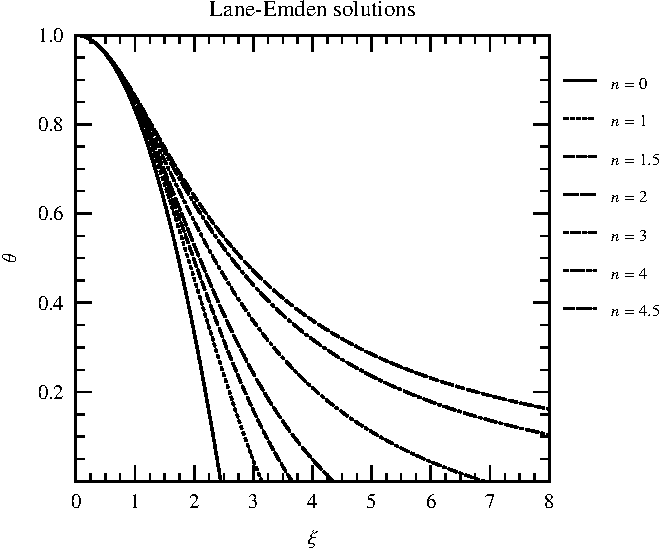
\includegraphics[width=4in]{LE_all.pdf}}
\caption{Solutions of the Lane-Emden equation for selected values of the index $n$.}
\label{f.LE-solutions}
\end{figure}

\section{Some Useful Relations}

First, let's get the mass of our polytropic sphere.  To do this, we write the integral
\[ M = \int_{0}^{R} 4\pi r^{2} \rho\,\dif r \]
and make the substitutions $r = r_{n}\xi$, $R = r_{n}\xi_{1}$, and $\rho = \rho_{c}\theta^{n}(\xi)$ to obtain
\[
M = 4\pi r_{n}^{3}\rho_{c}\int_{0}^{\xi_{1}} \xi^{2}\theta^{n}(\xi)\,\dif\xi.
\]
Using equation~(\ref{e.LE}) , the integrand can be written as a perfect differential, so we get
\begin{equation}\label{e.LE-mass}
M = 4\pi r_{n}^{3} \rho_{c}\left(-\xi_{1}^{2} \theta_{1}'\right).
\end{equation}
Here I define the shorthand $\theta_{1}' \equiv \theta(\xi)|_{\xi=\xi_{1}}$.  Substituting $r_{n} = R/\xi_{1}$ and dividing by 3 allows us to get a formula relating the central density to the mean density,
\begin{equation}\label{e.LE-density-ratio}
\rho_{c} = \frac{3M}{4\pi R^{3}}\left(-\frac{\xi_{1}}{3\theta_{1}'}\right).
\end{equation}
For the solutions shown in Figure~\ref{f.LE-solutions}, we have the following values of $\rho_{c}/\bar{\rho}$, as shown in Table~\ref{t.LE-properties}.
As the index $n$ increases, the configuration becomes more and more concentrated toward the center.

\begin{table}[htpb]
\caption{Properties of the Lane-Emden solutions.\label{t.LE-properties}}
\begin{center}
\begin{tabular}{c|rrrrrrr}
\hline
$n$ & 0 & 1.0 & 1.5 & 2.0 & 3.0 & 4.0 & 4.5 \\
\hline\hline
$\xi_{1}$ & 2.449 & 3.142 & 3.654 & 4.353 & 6.897 & 14.972 & 31.836\\
$-\theta_{1}'$ & 0.8165 & 0.3183 & 0.2033 & 0.1272 & 0.04243 & 0.008018 & 0.001715\\
$\rho_{c}/\bar{\rho}$ & 1.00 & 3.29 & 5.99 & 11.41 & 54.18 & 622.4 & 6187.8\\
\hline
\end{tabular}
\end{center}
\end{table}

Starting from equation~(\ref{e.LE-mass}), we can substitute for $r_{n}$ using equation~(\ref{e.LE-length-scale}) and $\rho_{c}$ using equation~(\ref{e.LE-density-ratio}) to get an equation for the central pressure,
\begin{equation}\label{e.LE-PC}
P_{c} = \frac{GM^{2}}{R^{4}} \frac{1}{4\pi(n+1)(-\theta_{1}')^{2}}.
\end{equation}
For an ideal gas, $P_{c} = (\NA\kB/\mu)\rho_{c}T_{c}$ with $\mu$ being the mean molecular weight, we can solve for the central temperature,
\begin{equation}\label{e.LE-TC}
T_{c} = \left(\frac{\mu}{\NA\kB}\right)\left(\frac{GM}{R}\right)\frac{1}{(n+1)\xi_{1}(-\theta_{1}')}.
\end{equation}
Finally, starting from equation~(\ref{e.LE-PC}), substituting for $P_{c}$ using equation~(\ref{e.polytope}), and eliminating $\rho_{c}$ using equation~(\ref{e.LE-density-ratio}), we obtain a relation between mass and radius in terms of $K$ and $n$,
\begin{equation}\label{e.LE-mass-radius}
M^{1-1/n} = \left[\frac{K(n+1)}{G(4\pi)^{1/n}} \xi_{1}^{1+1/n}\left(-\theta_{1}'\right)^{1-1/n} \right] R^{1-3/n}.
\end{equation}
Alternatively, one could use this equation to fit $K$ to a star of known $M$ and $R$.

Finally, we can derive a formula for the gravitational energy of our polytropic sphere.  First, we can integrate the equation for the energy,
\[
E_{\mathrm{grav}} = -G\int_{0}^{M}\frac{m}{r}\,\dif m,
\]
by parts to obtain
\begin{equation}\label{e.polytrope-energy-1}
E_{\mathrm{grav}} = -\frac{GM^{2}}{2R} - \frac{1}{2}\int_{0}^{R}\frac{Gm^{2}}{r^{2}}\,\dif r = -\frac{GM^{2}}{2R} - \frac{1}{2}\int_{0}^{R} \frac{\dif\Phi}{\dif r} m\,\dif r.
\end{equation}
If we define our zero of energy to be such that $\Phi(R) = 0$, then we can integrate by parts again to obtain
\begin{equation}\label{e.polytrope-energy-2}
E_{\mathrm{grav}} = -\frac{GM^{2}}{2R} + \frac{1}{2}\int_{0}^{R} \Phi\,\dif m.
\end{equation}
We can rewrite the equation of hydrostatic equilibrium as
\[ \frac{\dif P}{\dif r} = -\frac{\dif\Phi}{\dif r} \rho \]
and use equation~(\ref{e.polytope}) to eliminate $P$ to obtain
\[ \frac{\dif\Phi}{\dif r} = (1+n) K \rho^{1/n} .\]
Integrating from a point in the star $r$ to $R$, and again using choosing $\Phi(R) = 0$, we obtain
\begin{equation}\label{e.polytrope-energy-3}
\Phi(r) = -(1+n)K\rho(r)^{1/n} = -(1+n)\frac{P(r)}{\rho(r)}.
\end{equation}
Inserting equation~(\ref{e.polytrope-energy-3}) into equation~(\ref{e.polytrope-energy-2}), we have
\begin{equation}\label{e.polytrope-energy-4}
E_{\mathrm{grav}} = -\frac{GM^{2}}{2R} - \frac{1+n}{2}\int_{0}^{M} \frac{P}{\rho}\,\dif m = -\frac{GM}{2R} + \frac{1+n}{6}E_{\mathrm{grav}},
\end{equation}
where we used equation~(\ref{e.virial-1}) to relate the integral of $P/\rho$ to $E_{\mathrm{grav}}$. Solving equation~(\ref{e.polytrope-energy-4}) for $E_{\mathrm{grav}}$ gives us the desired result,
\begin{equation}\label{e.polytrope-energy}
E_{\mathrm{grav}} = -\frac{3}{5-n} \frac{GM^{2}}{R}.
\end{equation}
Note that solutions with $n > 5$ have a positive gravitational energy.

\section{Exercises}\label{s.LE-exercises}
\begin{enumerate}
\item Derive equations~(\ref{e.LE-mass})--(\ref{e.LE-mass-radius}).

\item Explain what the mass-radius relation, eq.~(\ref{e.LE-mass-radius}), means for the cases $n=1$ and $n=3$.

\item For a fully convective star with an ideal gas equation of state, how is the polytropic constant $K$ related to the entropy? Derive a formula for $R$ in terms of $M$ and $s$ in this case.  What happens to the star if the entropy increases, i.e., heat is added to it?

\emph{Hint:} Recall from thermodynamics that the entropy per unit mass of an ideal gas is
\begin{equation}\label{e.exercise-entropy}
s = \frac{\kB \NA}{\mu}\left\{ \frac{5}{2} + \ln\left[\frac{\mu}{\rho\NA}\left(\frac{\mu\kB T}{2\pi\NA\hbar^{2}}\right)^{3/2}\right]\right\}.
\end{equation}

Use the Lane-Emden solution to compute the specific entropy, per unit mass, in terms of the central temperature $T$ and the stellar mass $M$: $s = s(T_{c},M)$.  From this expression,  compute the ``gravothermal'' specific heat
\begin{equation}\label{e.cstar}
c_{\star} = T_{c}\frac{\partial s(T_{c},M)}{\partial T_{c}},
\end{equation}
and comment on its physical significance.

\item We will see later that low-mass pre-main-sequence stars (including brown dwarfs) are fully convective and have nearly constant effective temperatures.  Use these facts to model their pre-main sequence contraction.  Assume $T_{\mathrm{eff}} = \mathrm{const.}$ so that the luminosity is $L = 4\pi R^{2} \sigma_{\mathrm{SB}} T_{\mathrm{eff}}^{4}$.
%\begin{enumerate}
%\item 

Use the appropriate polytropic relation for the energy of the protostar and assume that the luminosity is powered by contraction. From these assumptions, derive an equation for $R(t)$. What is the characteristic timescale for a star to contract? Scale your answer to $T_{\mathrm{eff}} = 3000\nsp\K$ and $M = 0.1\nsp\Msun$ (i.e., get an analytical solution in terms of the variables $\tilde{T} = [\Teff/3000\nsp\K]$ and $\tilde{M} = [M/0.1\nsp\Msun]$).

Compare your findings with more elaborate calculations.  You will find a review in \href{http://arxiv.org/abs/astro-ph/0006383}{``Theory of Low-Mass Stars and Substellar Objects,''} G. Chabrier and I. Baraffe, Ann.\ Rev.\ Astron.\ Astrophys.\ \textbf{38:} 337 (2000). 
%\item Using appropriate expressions for the central density and temperature, calculate the time required for a star just below the hydrogen burning limit (about $0.07\nsp\Msun$) to contract to a radius such that $\eF(\rho_{c}) = \kB T_{c}$, where $\eF$ is the Fermi energy, and compare with the evolutionary tracks in Chabrier \& Baraffe.
%\end{enumerate}
\end{enumerate}

% !TEX root = ./notes.tex
\chapter[Equation of State]{The Equation of State}\label{ch.equation-of-state}

In statistical equilibrium, we can describe a system of particles by a distribution function $f(\vp,\vx)\,\dif^{3}p\,\dif^{3}x$, such that the number of particles is
\begin{equation}\label{e.dist}
N = \int \dif^{3}p\,\dif^{3}x\nsp f(\vp,\vx),
\end{equation}
where the integration is over the phase spaces of momentum and position coordinates $(\vp,\vx)$. In an ideal gas, the particles do not interact. In such a case, the distribution function $f = f(\vp)$ does not depend on position.  The integration over $\dif^{3}x$ just gives a factor of the volume, so the number density is $n = \int\dif^{3}p f(vp)$.  From equation~(\ref{e.dist}), we can get our other thermodynamic quantities: for example.
\begin{eqnarray}
\frac{E}{V} \equiv u = \int  \varepsilon(\vp) f(\vp)\,d^{3}p &\qquad& \textrm{energy per unit volume;}\label{e.u}\\
P = \int  (\vp\vdot \bvec{e}_{z} )(\bvec{v}\vdot\bvec{e}_{z}) f(\vp)\,d^{3}p &\qquad& \textrm{pressure}.\label{e.P}
\end{eqnarray}
Here $\varepsilon$ is the particle energy and $v$ the velocity.

\section{An ideal Fermi gas}

For \emph{fermions}, particles with half-integer spin, it can be shown that
\begin{equation}\label{e.fermion}
f(p) = \frac{g}{(2\pi\hbar)^{3}} \left[\exp\left(\frac{\varepsilon-\mu}{\kB T}\right)+1\right]^{-1}.
\end{equation}
In this equation $\varepsilon(p)$ is the energy of a particle, $\mu$ is the \emph{chemical potential}, $T$ is the temperature, and $g$ denotes the number of particles that can occupy the same energy level (for spin-1/2 particles, $g=2$).  The connection to thermodynamics is via the relations
\[
\frac{1}{T} = \left(\frac{\partial S}{\partial E}\right)_{N,V},\qquad -\frac{\mu}{T} = \left(\frac{\partial S}{\partial N}\right)_{E,V},
\]
and 
\[
TS = PV - \mu N + E;
\]
these are derived in standard texts. Let's explore what happens in various limits.  

\subsection{Non-degenerate, non-relativistic limit}
First, let's take $K\equiv\exp(\mu/\kB T)\ll 1$. (In the literature, $K$ is called the \emph{fugacity}.) Then in equation~(\ref{e.fermion}), we see that the exponential term dominates.  If our system is isotropic, then $d^{3}p = 4\pi p^{2}dp$, and we'll use this substitution from now on.  We then have for the number density
\begin{equation}
n(\mu,T) = \frac{gK}{2\pi^{2}\hbar^{3}}\int_{0}^{\infty}\exp\left(-\frac{\varepsilon}{\kB T}\right) p^{2}dp.
\end{equation}
To do the integral, notice that since $2m\varepsilon = p^{2}$, we have $p^{2}\,dp = m(2m\varepsilon)^{1/2}\,d\varepsilon$; making the substitution $x = \varepsilon/(\kB T)$, we get
\begin{equation}\label{e.n-int}
n(\mu,T) = \frac{gK}{2\pi^{2}\hbar^{3}}\sqrt{2}(m\kB T)^{3/2}\int_{0}^{\infty} x^{1/2}e^{-x}\,dx.
\end{equation}
You have all struggled with this integral in your past, but to avoid unpleasant flashbacks, I will just tell you that it is $\sqrt{\pi}/2$.  So, we have our first result (but we still don't know what it means),
\begin{equation}\label{e.n-nondeg}
n(\mu,T) = K\left[g\left(\frac{m\kB T}{2\pi\hbar^{2}}\right)^{3/2}\right].
\end{equation}

Let's forge on a little further, though, and try to get the energy per unit voume $u$.  Once we have $u$, we know we can get the pressure from the relation for a non-relativistic gas, $P = 2/3\;u$.  Using equations~(\ref{e.u}) and (\ref{e.fermion}),
\begin{equation}
u(\mu,T) = \frac{gK}{2\pi^{2}\hbar^{3}}\int_{0}^{\infty}\exp\left(-\frac{\varepsilon}{\kB T}\right) \varepsilon p^{2}dp.
\end{equation}
Let's repeat our trick of changing variables from $p$ to $x = \varepsilon(p)/\kB T$; we then have
\begin{equation}
u(\mu,T) = \frac{gK}{2\pi^{2}\hbar^{3}}\sqrt{2}m(m\kB T)^{3/2}\int_{0}^{\infty} x^{3/2}e^{-x}\,dx.
\end{equation}
Did you notice that if we integrate by parts,
\[
\int_{0}^{\infty} x^{3/2}e^{-x}\,dx =  \frac{3}{2}\int_{0}^{\infty}x^{1/2}e^{-x}\,dx = \frac{3}{4}\sqrt{\pi},
\]
we get the integral we already solved in equation~(\ref{e.n-int})?  Putting everything together and using the expression for $n$ (eq.~[\ref{e.n-nondeg}]), we have
\begin{equation}
u(\mu,T) = \frac{3}{2}\left\{K\left[g\left(\frac{m\kB T}{2\pi\hbar^{2}}\right)^{3/2}\right] \right\}\kB T = \frac{3}{2}n\kB T.
\end{equation}
which gives us the pressure,
\begin{equation}\label{e.PVnkT}
P = \frac{2}{3} u = n \kB T.
\end{equation}
Whoo-hoo!  We've rediscovered the ideal gas.

Now we have to understand this chemical potential $\mu$.  We can solve equation~(\ref{e.n-nondeg}) for $\mu$,
\begin{equation}\label{e.fugacity-nondeg}
\exp\left(\frac{\mu}{\kB T}\right) = K = n\left[g\left(\frac{m\kB T}{2\pi\hbar^{2}}\right)^{3/2}\right]^{-1}.
\end{equation}
Now $K$ is dimensionless, a number, so the thing in $[\;]$ must have dimensions of number density.  Let's call it $n_{Q}$.  Our chemical potential is then $\mu = \kB T\ln(n/n_{Q})$.  To understand the significance of $n_{Q}$, let's calculate the uncertainty in position of a particle having energy $\kB T$; from Heisenberg, we have
\[
\Delta x \approx \frac{\hbar}{\Delta p} \sim \frac{\hbar}{\sqrt{m\kB T}}
\]
where I am dropping numerical factors and I've made the substitution $\Delta p\sim p \approx \sqrt{m\kB T}$.  Now what happens if I pack the particles so that on average there are $g$ particles per box of volume $(\Delta x)^{3}$?  In that case the density would be $n = g(\sqrt{m\kB T}/\hbar)^{3} \approx n_{Q}$.  So, what appears in the chemical potential is the ratio of the density to that density at which the particles are packed so closely that the uncertainty in their positions is the same size as the typical inter-particle spacing.
In the ideal-gas limit $K \ll 1$, which makes sense: $n\ll n_{Q}$, so the particles are very far apart compared to their thermal de Broglie wavelengths, and quantum effects ought to be unimportant.

\subsection{Degenerate, non-relativistic limit}\label{s.deg-limit-fermions}
When $n\gtrsim n_{Q}$, we can no longer use the approximation $K \ll 1$, so let's go to the opposite limit, for which $\mu \gg \kB T$.  In this case, notice from equation~(\ref{e.fermion}) that
\begin{equation}
f(p) \approx \frac{g}{(2\pi\hbar)^{3}}\left\{\begin{array}{lr} 1 & \varepsilon < \mu\\ 0 & \varepsilon> \mu\end{array}\right. .
\end{equation}
We can think of this as inserting $g$ particles in each energy level, starting with the lowest energy level and continuing until all of the particles are used. The last particle is inserted with energy $\varepsilon \approx \mu$.  The only levels that will be partially filled will be those lying in a thin band $\varepsilon \approx\mu \pm \kB T$.  If that is the case, we can make the following approximation.  Let's take the limit $T \to 0$, and define the \emph{Fermi energy} by $\eF = \mu|_{T\to 0}$ and the \emph{Fermi momentum} by $\pF = \sqrt{2m\eF}$.  We can then write equation~(\ref{e.dist}) as
\begin{equation}
n(\mu) = \frac{1}{\pi^{2}\hbar^{3}}\int_{0}^{\pF} p^{2} dp,
\end{equation}
since the integrand is zero for $p > \pF$.  The main application is for electrons, which are spin one-half, so we substitute $g = 2$. Now this is an easy integral,
\begin{equation}\label{e.n-deg}
n(\mu) = \frac{\pF^{3}}{3\pi^{2}\hbar^{3}} = \frac{(2m\eF)^{3/2}}{3\pi^{2}\hbar^{3}},
\end{equation}
or $\mu \approx \eF = (3\pi^{2}n)^{2/3} \hbar^{2}/(2m)$.  Let's get the energy per unit volume and the pressure,
\begin{equation}
u(\mu) = \frac{1}{\pi^{2}\hbar^{3}}\int_{0}^{\pF} \frac{p^{2}}{2m}\,p^{2}\,dp = \frac{\pF^{5}}{5\pi^{2}\hbar^{3}}.
\end{equation}
Comparing this with equation~(\ref{e.n-deg}), we have
\begin{eqnarray}
u &=& \frac{3}{5}n\eF,\label{e.u-deg}\\
P &=& \frac{2}{5}n\eF\label{e.P-deg}.
\end{eqnarray}
To lowest order, neither $u$ nor $P$ depend on $T$.  Substituting for \eF\ in equation~(\ref{e.P-deg}) gives us the equation of state,
\begin{equation}\label{e.eos-deg}
P = \frac{2}{5}\left(3\pi^{2}\right)^{2/3}\frac{\hbar^{2}}{2m}n^{5/3}.
\end{equation}
Notice that in equation~(\ref{e.fugacity-nondeg}), $n_{Q}\propto m^{3/2}$.  This means that at any given temperature, $n_{Q}$ for electrons is $1836^{3/2} = 80,000$ times smaller than it is for protons, not to mention helium or heavier nuclei. As a result, the electrons will become degenerate ($n\gtrsim n_{Q}$) at a much lower mass density than the ions.    A common circumstance, then, is to have a mixture of degenerate electrons and ideal ions (we will deal with non-ideal corrections due to electric forces later).  

Now, let's estimate the boundary between the non-degenerate and degenerate regimes. At a given temperature, we know in the low-density limit that the electrons obey the ideal gas law (eq.~[\ref{e.PVnkT}]) and in the high-density limit the electrons are degenerate (eq.~[\ref{e.eos-deg}]). So, let's extrapolate our two limiting expressions for the pressure and see where they meet,
\begin{equation}
n_{e}\kB T = P_{e,\mathrm{ideal}} \sim P_{e,\mathrm{deg.}} 
  = \frac{2}{5}n_{e}\eF,
\end{equation}
or $\eF \approx \kB T$.  No surprise here.  Notice that the ratio
\begin{equation}
\frac{\eF}{\kB T} \sim \frac{(3\pi^{2})^{2/3}\hbar^{2}}{2m_{e}\kB T}n_{e}^{2/3} \sim \left(\frac{n_{e}}{n_{Q}}\right)^{2/3},
\end{equation}
so marking the onset of degeneracy with $\eF\sim \kB T$ also makes sense from that aspect as well. Our boundary in the density-temperature plane between the non-degenerate and degenerate regimes is then determined by setting $\kB T = \eF$,
\begin{equation}\label{e.TF}
T = \frac{(3\pi^{2})^{2/3}\hbar^{2}}{2m_{e}\kB }\left(\frac{Y_{e}\rho}{\mb}\right)^{2/3} = 3.0\ee{5}\nsp\K \left(Y_{e}\rho\right)^{2/3}.
\end{equation}
If the temperature falls below this value, the electrons will be degenerate. Here $Y_{e}$ is the electron molar fraction, or electron abundance and \mb\ is the atomic mass unit; consult \S\ref{s.composition} for details.

\section{Fermi-Dirac integrals}
This condition for the onset of degeneracy, eq.~(\ref{e.TF}), is only a rule-of-thumb; in any serious calculation we would want to calculate the electron thermal properties from the exact integrals
\begin{eqnarray}\label{e.FD12}
n(\mu,T) &=& \frac{\sqrt{2}(m\kB T)^{3/2}}{\pi^{2}\hbar^{3}}\int_{0}^{\infty} \frac{x^{1/2}\,dx}{\exp(x-\psi)+1} \\
P(\mu,T) &=& \frac{(2m\kB T)^{3/2}(\kB T)}{3\pi^{2}\hbar^{3}}\int_{0}^{\infty} \frac{x^{3/2}\,dx}{\exp(x-\psi)+1},
\end{eqnarray}
where $\psi = \mu/(\kB T)$.  These integrals cannot be done analytically, but they occur so frequently that there are many published tables and numerical approximation schemes \citep[see][]{timmes.swesty:accuracy}.  Specifically, the \emph{non-relativistic Fermi-Dirac integral of order $\nu$} is defined as
\begin{equation}\label{e.FDintegral}
F_{\nu}(\psi) = \int_{0}^{\infty}\frac{ x^{\nu}\,dx}{\exp(x-\psi)+1}.
\end{equation}
One can (numerically) invert equation~(\ref{e.FD12}) to solve for the chemical potential $\psi \kB T$.

The general case for a relativistic Fermi gas is left as an exercise.

\section{Relativistic photon gas}\label{s.relativistic-photon-gas}
Photons are \emph{bosons}---they have spin 1. For bosons, the distribution function is similar to that in equation~(\ref{e.fermion}), but with the $+1$ replaced by $-1$ in the denominator. In addition, photon number is not conserved: one can freely create and destroy photons.  This implies that their chemical potential is zero.  Also, $g=2$ for photons: there are two independent polarization modes. Putting all of these together, we can write energy per unit volume as
\begin{equation}\label{e.boson-dist}
u = \frac{1}{\pi^{2}\hbar^{3}}\int_{0}^{\infty}\varepsilon p^{2}\left[\exp\left(\frac{\varepsilon}{\kB T}\right)-1\right]^{-1}\,dp.
\end{equation}
Now, use the fact that $p = \varepsilon/c$ and change variables to $x = \varepsilon/(\kB T)$ to get
\[
 u = \frac{\kB ^{4}T^{4}}{\pi^{2}c^{3}\hbar^{3}}\int_{0}^{\infty} \frac{x^{3}\,dx}{e^{x}-1}.
\]
This integral is a classic and is equal to $\pi^{4}/15$.  Hence the energy per unit volume and the pressure are
\begin{eqnarray}\label{e.radiation-eos}
u &=& \left(\frac{\kB ^{4}\pi^{2}}{15 c^{3}\hbar^{3}} \right) T^{4} = aT^{4}\\
P &=& \frac{1}{3} aT^{4}.
\end{eqnarray}
In CGS units, $a = 7.566\ee{-15}\nsp\ergs\usp\cm^{-3}\usp\K^{-4}$.

\section{Connection to thermodynamics}
Once we have the distribution functions, we can get all of the other thermodynamic properties from the thermodynamic relations: in what follows let $N = nV$ be the total number of particles, with $V$ being the volume of the system.  The total energy is then $E = uV$, and the entropy is $S$, and we have
\begin{eqnarray}
F = E - TS, &\qquad& \textrm{Helmholtz free energy,}\\
H = E + PV, &\qquad& \textrm{Enthalpy,}\\
\mu N = G = A + PV, &\qquad& \textrm{Gibbs free energy}.
\end{eqnarray}
For example, we have in the non-degenerate limit that
\begin{equation}\label{e.chem-pot-ideal-gas}
\mu = \kB T\ln K = \kB T\ln\left[ \frac{n}{g}\left(\frac{2\pi\hbar^{2}}{m\kB T}\right)^{3/2}\right],
\end{equation}
and so we could write the entropy per unit mass as
\begin{eqnarray}
s \equiv \frac{S}{Nm} &=& \frac{1}{Nm}\frac{E + PV - \mu N}{T}\nonumber\\
 &=& \frac{\kB }{m}\left\{ \frac{5}{2} + \ln\left[\frac{g}{n}\left(\frac{m\kB T}{2\pi\hbar^{2}}\right)^{3/2}\right]\right\}.
\label{e.sacker-tetrode}
 \end{eqnarray}
In this equation I have used the ideal non-degenerate values $E = (3/2) N\kB T$, $PV = N\kB T$ and have denoted the mass per particle as $m$ and the degeneracy of the spin-states as $g$.

\section{Chemical Equilibrium: The Saha Equation}

Consider a reaction, $A + B + \ldots \to C + D + \ldots$. When this reaction comes into equilibrium, we are at a maximum in entropy, and the condition for equilibrium is that the energy cost, at constant entropy to run the reaction in the forward direction is the same as to run the reaction in reverse. This can be expressed in terms of chemical potentials as
\begin{equation}\label{e.mass-action}
\mu_{A} + \mu_{B} + \ldots \to \mu_{C} + \mu_{D} + \ldots
\end{equation}
Note in this formalism that a reaction $2A \to B$ would be expressed as $2\mu_{A} = \mu_{B}$.

As a worked example, we consider the ionization equilibrium of hydrogen,
\[ \mathrm{H^{+}} + e \to \mathrm{H}. \]
To use equation~(\ref{e.mass-action}), we need to have both sides on the same energy scale. The reaction in the exothermic direction; that is, heat is evolved if the reaction proceeds as written.  This means that the right-hand side is more bound, and its minimum energy is less than that of the right-hand side. To get both sides on the same energy scale, we must subtract the binding energy, $Q=13.6\nsp\eV$, from the right-hand side:
\begin{equation}\label{e.ionization-chem-potential}
\mu_{+} + \mu_{-}= \mu_{0} -  Q.
\end{equation}
Another way to see why $Q$ appears is to add the rest mass for each species to its chemical potential; collecting all terms on the right, we would then have a term $(m_{0}-m_{+}-m_{-})c^{2} = -Q$. Some ionization potentials, along with the half-ionization temperature for a given electron number density $n_{e}$, are given in Table~\ref{t.ionization-potentials}.

\begin{table}[htpb]
\begin{center}
\caption{Selected ionization potentials and half-ionization temperatures}\label{t.ionization-potentials}
\begin{tabular}{l|rrrr}
\hline
element & H$^{-}$ & Na & H & He\\
\hline\hline
$Q/(\mathrm{eV})$ & 0.75 & 5.14 & 13.6 & 24.6\\
$T_{1/2}(n_{e} = 10^{13}\nsp\cm^{-3})/\mathrm{K}$ & 600 & 3300 & 8\,000 & 13\,900\\
$T_{1/2}(n_{e} = 10^{16}\nsp\cm^{-3})/\mathrm{K}$ & 900 & 5\,000 & 11\,800 & 20\,200\\
\hline
\end{tabular}
\end{center}
\end{table}

For a non-degenerate plasma, we can insert eq.~(\ref{e.chem-pot-ideal-gas}) into eq.~(\ref{e.ionization-chem-potential}), divide through by $\kB T$, and take the exponential to obtain
\begin{equation}\label{e.saha-eqn}
\frac{n_{+}n_{-}}{n_{0}} = \frac{g_{+}g_{-}}{g_{0}}\left(\frac{m_{-}\kB T}{2\pi\hbar^{2}}\right)^{3/2}\exp\left(-\frac{Q}{\kB T}\right).
\end{equation}
The number density of all hydrogen in the gas is $n_{0}+n_{+} = n_{\mathrm{H}}$.  Denote the ionized fraction by $x = n_{+}/n_{\mathrm{H}} = n_{i}/n_{\mathrm{H}}$, so that the left-hand side of equation~(\ref{e.saha-eqn}) is $n_{\mathrm{H}} x^{2}/(1-x)$. In the hydrogen atom ground state, the electron spin and proton spin are either aligned or anti-aligned. These states are very nearly degenerate, so that $g_{0} = 2$.  Both the proton and electron have spin $1/2$; there are really only two available states, however, because of the freedom in choosing our coordinate system.  As a result, $g_{+}g_{-} = 2$ as well.

Inserting these factors into equation~(\ref{e.saha-eqn}), and using $\kB = 8.6173\ee{-5}\nsp\eV/\K$, we obtain
\begin{equation}\label{e.saha-reduced}
\frac{x^{2}}{1-x} = \frac{2.41\ee{21}\nsp\cm^{-3}}{n_{\mathrm{H}}} \left(\frac{T}{10^{4}\nsp\K}\right)^{3/2}\exp\left(-\frac{15.78\ee{4}\nsp\K}{T}\right).
\end{equation}
This equation defines a set of points in the $\rho-T$ plane for which $x = 1/2$.  We may take this set of points to mark the boundary between neutral and ionized hydrogen. At fixed density, the transition from neutral to fully ionized is very rapid.

\section{Coulomb interactions}
Under the conditions in a stellar interior, most of the atoms are ionized, and the stellar matter consists of positively charged nuclei and ions and negatively charged electrons. A \emph{plamsa} is defined as a gas of charged particles in which the kinetic energy of a typical particle is much greater than the potential energy due to its nearest neighbors. To make this quantitative, consider a gas with only one species present, with charge $q$.  Let the mean spacing between particles be $a$; clearly the number density of such particles is $n = (4\pi a^{3}/3)^{-1}$.  We may then take the quantity
\begin{equation}\label{e.Gamma-definition}
\Gamma \equiv \frac{q^{2}}{a\kB T}
\end{equation}
as indicating the relative importance of potential to kinetic energy.  In a classical plasma, $\Gamma \ll 1$.  Note, however, that systems with $\Gamma > 1$ are often (confusingly) called  \emph{strongly coupled plasmas}. The meaning is usually clear from context.

\subsection{Debye shielding}\label{s.plasma-shielding}

Imagine a typical charged particle in a plasma.  Very close to the particle, we expect the electrostatic potential to be that of an isolated charge $\Phi = q/r$. Far from the particle, there will be many other particles surrounding it, and the potential is screened. For example, a positive ion will tend to attract electrons to be somewhat, on average, closer to it than other ions: we say that the ion \emph{polarizes} the plasma.  As a result of this polarization, the potential of any particular ion should go to zero much faster than $1/r$ due to the ``screening'' from the enhanced density of opposite charges around it.

Let's consider a plasma having many ion species, each with charge $Z_{i}$, and elections. About any selected ion $j$,  particles will arrange themselves according to Boltzmann's law,
\begin{equation}\label{e.ion-boltzmann}
n_{i}(r) = n_{i0}\exp\left[-\frac{Z_{i}e\Phi(r)}{\kB T}\right].
\end{equation}
Here $n_{i0}$ is the density of particle $i$ far from the charge $j$, and $r$ is the distance between particles $i$ and $j$.  (A similar equation holds for the electrons, with $Z$ replaced by $-1$.) To solve for the potential, we can use Poisson's equation,
\begin{equation}\label{e.Poisson}
\nabla^{2}\Phi = -4\pi \sum_{i} Z_{i}e n_{i}(r) +4\pi e n_{e}(r).
\end{equation}
Our assumption is that the term in the exponential of equation~(\ref{e.ion-boltzmann}) is small, so we may expand it to first order in $\Phi$ and substitute that expansion into equation~(\ref{e.Poisson}) to obtain in spherical geometry
\[
 \frac{1}{r}\frac{\partial^{2}}{\partial r^{2}}\left(r\Phi\right) = -4\pi e \left[\sum_{i} n_{i0}Z_{i}\left(1-\frac{Z_{i}e\Phi}{\kB T}\right) - n_{e0}\left(1 + \frac{e\Phi}{\kB T}\right)\right].
\]
The overall charge neutrality of the plasma implies that $n_{e0} = \sum_{i}Z_{i}n_{i0}$; using this to simplify the above equation gives
\begin{equation}\label{e.linearized-Poisson}
\frac{1}{r}\frac{\partial^{2}}{\partial r^{2}}\left(r\Phi\right) = \left[\frac{4\pi e^{2}}{\kB T}\sum_{i} n_{i0}\left(Z_{i}^{2}+Z_{i}\right)\right]\Phi \equiv \lambdaD^{-2}\Phi.
\end{equation}
The quantity in $[\, ]$ has dimensions of reciprocal length squared and we define it as $(1/\lambdaD)^{2}$ with $\lambdaD$ being called the \emph{Debye length}.

Multiplying equation~(\ref{e.linearized-Poisson}) by $r$, integrating twice, and determining the constant of integration from the condition that as $r\to 0$, $\Phi \to Z_{j}e/r$ gives the self-consistent potential
\begin{equation}\label{e.screened-potential}
\Phi = \frac{Z_{j}e}{r}\exp\left(-\frac{r}{\lambdaD}\right).
\end{equation}
The Debye length \lambdaD\ determines the size of the screening cloud around the ion.

In order for the above derivation to be valid, we require that $\lambdaD \gg a$, where $a$ is the mean ion spacing; otherwise, there won't be any charges in our cloud to screen the potential! Equivalently, we require the number of particles in a sphere of radius \lambdaD\ to be large,
\begin{equation}\label{e.plasma-parameter}
\frac{4\pi}{3}\lambdaD^{3} \sum_{i} n_{i} \gg 1.
\end{equation}
This condition must hold if we are to treat the gas as a plasma. In the exercises you are asked to show that this condition is equivalent to $\Gamma \ll 1$.

\subsection{Corrections to the ideal gas EOS}\label{s.plasma-corrections}

In a plasma the particles are not independent: shake one particle and other nearby particles will shake as well. In statistical mechanics, this requires introducing \emph{correlation functions} to derive the equation of state.  We'll adopt the more intuitive approach of Debye and H\"uckel to get the lowest-order correction to the ideal gas EOS.  First, the total electrostatic energy in a volume $V$ is
\begin{equation}\label{e.electrostatic-energy}
E_{\mathrm{Coul}} = \frac{1}{2}V\sum_{j}Z_{j}e n_{j}\Phi_{j}.
\end{equation}
Here $\Phi_{i}$ is the potential at a particle $j$ \emph{due to all the other particles in the plasma.}  Now, we computed the total potential around a particle (eq.~[\ref{e.screened-potential}]); expanding and subtracting off the self-potential of particle $j$ gives $\Phi_{j} = -Z_{j}e/\lambdaD$.  Inserting this into equation~(\ref{e.electrostatic-energy}) and expanding gives
\begin{equation}\label{e.electrostatic-energy-2}
E_{\mathrm{Coul}} \approx - V\left(\frac{\pi}{\kB T}\right)^{1/2} e^{3} \left[\sum_{i}n_{i0} \left(Z_{i}^{2} + Z_{i}\right)\right]^{3/2}.
\end{equation}
This energy is to be added to the kinetic energy of the gas.  The effect of the electrostatic interactions is to \emph{decrease} the energy in the gas, that is, to make it more bound.

We can't directly get the pressure from equation~(\ref{e.electrostatic-energy-2}) because the equation isn't in terms of $S$ and $V$ (recall that $P = -(\partial E/\partial V)_{S}$) but rather in terms of $T$ and $V$.
In order to get the pressure, we first must find the Helmholtz free energy $F$. To do this, we integrate the thermodynamical identity
\[ E = -T^{2}\left(\frac{\partial}{\partial T}\right)_{V}\left(\frac{F}{T}\right)
\] 
and then take $P = -(\partial F/\partial V)_{T,N}$ to obtain
\begin{equation}\label{e.pressure-correction}
 P_{\mathrm{Coul}} \approx -\frac{e^{3}}{3}\left(\frac{\pi}{\kB T}\right)^{1/2}\left[\frac{\left(\langle Z^{2}\rangle+\langle Z\rangle \right)\rho}{\langle A\rangle\mb}\right]^{3/2}.
\end{equation}
The effect of Coulomb interactions is to decrease the pressure below the ideal gas value.

\subsection[Strongly Coupled Plasmas]{Coulomb corrections when the electrons are degenerate}\label{s.degenerate-coulomb}

The above discussion holds only when both the electrons and ions are non-degenerate.  What happens when the electrons are degenerate?  In that case the kinetic energy is of order the Fermi energy, not the temperature.  We might think to replace $\kB T$ with \eF\ in equation~(\ref{e.Gamma-definition}). Recalling the formula for \eF\ from \S~\ref{s.deg-limit-fermions}, we have the condition for the Coulomb interactions to be weak,
\begin{equation}\label{e.condition-weak-degen}
\frac{e^{2}}{a \eF} = \left(\frac{4\pi n}{3}\right)^{1/3}\left(\frac{m_{e} e^{2}}{\hbar^{2}}\right)\frac{2}{(3\pi^{2} n)^{2/3}} < 1.
\end{equation}
Here $m_{e}$ and $n$ denote, respectively, the electron mass and number density.  Do you recognize the quantity $\hbar^{2}/(m_{e}e^{2})$?  It is the Bohr radius, \abohr.  What is \abohr\ doing in this equation?  Well, we are looking for a quantum mechanical system in which the Coulomb interaction is comparable to the non-relativistic kinetic energy.  Does that sound like any system you've seen before?

Cleaning up equation~(\ref{e.condition-weak-degen}), our condition for the electrons to be weakly interacting when degenerate is
\begin{equation}
\left(\frac{2^{5/3}}{3\pi}\right)\left( n \abohr^{3}\right)^{-1/3} < 1,
\end{equation}
or, in terms of mass density $\rho$ and electron fraction $Y_{e}$, $(Y_{e}\rho) > 0.4\nsp\grampercc$.  As the density increases, the electron gas becomes more ideal, that is, the electrostatic interaction matters less and less.  

Just to complete the discussion on electrons, what if the electrons are relativistic?  In this case, $\eF = \pF c = (3\pi^{2}n)^{1/3}\hbar c$, and
\begin{equation}\label{e.condition-weak-rel-degen}
\frac{e^{2}}{a \eF} = \left(\frac{4}{9\pi}\right)^{1/3}\left(\frac{e^{2}}{\hbar c}\right) = 3.8\ee{-3}.
\end{equation}
In this case $\eF \propto n^{1/3}$ so the density dependence cancels.  You will note the appearance of the fine structure constant $\alpha_{\mathrm{F}} = e^{2}/(\hbar c)$, as you might have expected when dealing with relativistic electrons and electrostatics.

Under astrophysical conditions, we can almost always regard degenerate electrons as being ideal.  What about the ions?  They are not usually degenerate under conditions of interest. We can get a simple expression if we go to the opposite limit, in which the electrons are very degenerate.  In that case, the electrons are an ideal gas and hence have uniform density. If the temperature is low enough, the ions will have $Z^{2}e^{2}/(a\kB T) \gg 1$; in this case we might expect the ions will arrange themselves into a lattice that maximizes the inter-ionic spacing.

To get an estimate of the electrostatic energy, let's compute the energy of a charge-neutral sphere centered on a particular ion of charge $Z_{i}$.  Because the electrons have a uniform density, $Y_{e}\rho/\mb$, we can find the radius of the sphere $a$ by requiring it to have $Z_{i}$ electrons,
\begin{equation}\label{e.radius-ion-sphere}
\frac{4\pi}{3}a^{3}\left(Y_{e}\frac{\rho}{\mb}\right) = Z_{i},
\end{equation}
or $a = [3 Z_{i} \mb/(4\pi Y_{e}\rho)]^{1/3}$.  The potential energy of this sphere has two components. The first is due to electron-electron interactions,
\begin{equation}\label{e.ee-energy}
E_{ee} = \int_{0}^{a} \frac{q(r)\, \dif q}{r} = \frac{3}{5}\frac{Z_{i}^{2}e^{2}}{a},
\end{equation}
where $q(a) = Z_{i}e(r/a)^{3}$ is the charge in a sphere of radius $r < a$. The second component of the potential energy is due to the ion-electron interaction,
\begin{equation}\label{e.ei-energy}
E_{ei} = -Z_{i}e\int_{0}^{a}\frac{\dif q}{r} = -\frac{3}{2}\frac{Z_{i}^{2}e^{2}}{a}.
\end{equation}
Combining equations~(\ref{e.ee-energy}), (\ref{e.ei-energy}), and (\ref{e.radius-ion-sphere}) gives the total electrostatic energy for a single ion-sphere,
\begin{equation}\label{e.madelung-sphere}
E = -\frac{9}{10} \frac{Z_{i}^{2}e^{2}}{a} = -\frac{9}{10} Z_{i}^{5/3} e^{2} \left(\frac{4\pi}{3}\frac{Y_{e}\rho}{\mb}\right)^{1/3}.
\end{equation}
Multiplying this by $n_{i} = Y_{i}\rho/\mb$, summing over all ion species $i$, and defining $\langle Z^{5/3}\rangle = n^{-1}\sum Z_{i}^{5/3}n_{i}$ where $n = \sum n_{i}$, gives the total Coulomb energy per volume,
\begin{equation}\label{e.madelung-total}
E_{\mathrm{Coul}} = -\frac{9}{10} n\kB T \left[\frac{\langle Z^{5/3}\rangle e^{2}}{\kB T}\left(\frac{4\pi}{3}\frac{Y_{e} \rho}{\mb}\right)^{1/3}\right].
\end{equation}
Notice that the quantity in $[\nsp]$ reduces to $\Gamma$ for a single-species plasma.  If we therefore define $\Gamma \equiv [\nsp]$ for a multi-component plasma, we have $E_{\mathrm{Coul}} \approx -0.9 n\kB T \Gamma$; the pressure is then $P_{\mathrm{Coul}} = E_{\mathrm{Coul}}/3  = -0.3 n \kB T \Gamma$. This holds in the limit $\Gamma \gg 1$.

\section{Exercises}\label{s.EOS-exercises}
\begin{enumerate}
\item For an isotropic momentum distribution, show that 
\[
P = \frac{1}{3}\int |p||v| f(\vp)\,\dif^{3}\vp.
\]
\item Now show that for a non-relativistic gas, $P = (2/3)E/V$, and that for a relativistic gas, $P = (1/3)E/V$.

\item Repeat the derivation of equation~(\ref{e.u-deg}) and (\ref{e.P-deg}) for  a relativistic Fermi gas. What is the expression for the temperature at which the gas becomes degenerate (cf.~eq.~[\ref{e.TF}]) in this case?

\item Get the first order corrections to the Maxwell-Boltzmann gas. Take the fugacity $K \ll 1$, and expand the Fermi-Dirac distribution  (eq.~[\ref{e.fermion}]) to lowest order in $K\exp[-\varepsilon/(\kB T)]$. Show that 
\begin{eqnarray*}
 n(K,T) &=& n_{0}\left(1 - 2^{-3/2}K\right) \\
 u(K,T) &=& \frac{3}{2}n_{0}\kB T \left(1-2^{-5/2}K\right),
\end{eqnarray*}
where $n_{0}$ is the density in the limit $K\to 0$.
Then derive the equation of state $P = P(n,T)$ to lowest order in $K$. For a given ($n, T$), is the pressure larger or smaller than that of the ideal Maxwell-Boltzmann limit?

\item In an external field (i.e., gravitational) the chemical potential, which is the change in energy when the number of particles is increased, must include the potential.  Consider an ideal gas in a planar atmosphere of  constant gravitational acceleration $g$.  Write the chemical potential as $\mu(z)  = \mu_{\mathrm{id}} + \Phi$, where $\mu_{\mathrm{id}}$ is the chemical potential for an ideal gas in the absence of gravity, and $\Phi$ is the gravitational potential.  For an atmosphere in complete equilibrium ($\mu = \mathrm{const}$, $T = \mathrm{const}$), calculate the pressure as a function of position, $P = P(z)$, and show that it agrees with considerations from hydrostatic balance, equation~(\ref{e.planar-hydrostatic}).

\item 
\begin{enumerate}
\item Solve equation~(\ref{e.saha-reduced}) for a density of $10^{16}\nsp\cm^{-3}$ (a fiducial value for the solar photosphere) and find the half-ionization temperature, i.e., the temperature at which $x=0.5$.  Explain the reason for the discrepancy between the half-ionization temperature and $\kB T = 13.6\nsp\eV$.

\item At this half-ionization temperature, what is the occupancy of the excited levels of the hydrogen atom?  Do we need to worry about corrections to the ionization from these excited states?
\end{enumerate}

\item Show that equation~(\ref{e.plasma-parameter}) is equivalent to $\Gamma \ll 1$ for a single species plasma.

\item Show that for a non-relativistic plasma, the magnetic interaction between two charged particles is much less than the electrostatic interaction.

\item Show that the net charge in the shielding cloud about an ion of charge $Ze$ is $-Ze$; the shielding cloud cancels out the ion's charge.

\item 
\begin{enumerate} 
\item\label{p.zero-pressure-iron} In the zero-temperature limit (electrons are fully degenerate) use the charge-neutral sphere approximation (p.~\pageref{e.madelung-total}) to calculate the density at which completely ionized \iron[56] has zero pressure.

\item Estimate the pressure that would be required to compress \iron[56] at the density found in part~\ref{p.zero-pressure-iron}.
\end{enumerate}

\item Now write the total pressure as the sum of electron and Coulomb pressure, and use the virial scalings that we derived for pressure and density in terms of mass and radius, to obtain a relation between mass and radius for a cold object (``a rock'').  Find the mass having the largest radius, and express this mass in terms of fundamental physical constants.  How does it compare with the mass of Jupiter?  Scale the mass and radii to that of Jupiter, and plot $R(M)$ for pure \hydrogen, pure \helium, and pure \carbon\ objects.  Also indicate on this plot the masses and radii of the Jovian planets for comparison.

\end{enumerate}

% !TEX root = ./notes.tex
\chapter{Notes on Radiation Transport}

\newcommand{\unitvector}[1]{\ensuremath{\bvec{\hat{#1}}}}
\newcommand{\unitn}{\unitvector{n}}
\newcommand{\unitk}{\unitvector{k}}
\newcommand{\Ledd}{\ensuremath{L_{\mathrm{Edd}}}}
\newcommand{\Prad}{\ensuremath{P_{\mathrm{rad}}}}
\newcommand{\Pgas}{\ensuremath{P_{\mathrm{gas}}}}


The sun is very opaque.  Were photons able to stream freely, they would exit in $\sim \Rsun/c = 2.0\nsp\second$.  We saw that is instead takes millions of years for the sun to radiate away its stored thermal energy (see eq.~[\ref{e.K-H}]).  As a result, we can regard the sun as a cavity filled with photons with a very slight leakage.  This is the description commonly invoked to describe blackbody radiation, and we expect that in the interior of the sun, the radiation can be described by a photon gas in thermal equilibrium at the ambient temperature.

\section{Description of the Radiation Field}

Consider a cavity containing a gas of photons. In general we can describe the mean number of photons in this cavity as
\begin{equation}\label{e.photon-occupation}
 N = \frac{2}{h^{3}}\int f(p,x)\,\dif^{3}x\,\dif^{3}p.
\end{equation}
Here $f$ is a distribution function; if we are in thermal equilibrium, $f$ is the Bose-Einstein distribution, but our discussion will be more general.  Now consider a small surface on our cavity with area $\dif A$ and unit normal $\unitn$.  The energy incident on this area in a time $\dif t$ having propagation vector along $\unitn$ and propagating into solid angle $\dif\Omega$ is found by integrating equation~(\ref{e.photon-occupation}) over a volume $c\dif t\,\dif A$,
\[
\dif E = \dif A\,c\dif t\,\dif\nu\,\left( \frac{2}{h^{3}}p^{2}\dif p\,\dif\Omega\right)  h\nu \, f.
\]
Since the photon momentum is $p = h\nu/c$, we have
\begin{equation}\label{e.specific-intensity}
I_{\nu} \equiv \frac{\dif E}{\dif t\,\dif A\,\dif\Omega\,\dif\nu} = \frac{2h\nu^{3}}{c^{2}} f.
\end{equation}
This defines the \emph{specific intensity} $I_{\nu}$.  It is easy to show that in the absence of interactions with matter, $I_{\nu}$ is conserved along a ray.  If the photons are in thermal equilibrium, then we can replace $f$ with the Bose-Einstein distribution,
\begin{equation}\label{e.Bnu}
B_{\nu} \equiv \frac{2 h\nu^{3}}{c^{2}} \left[\exp\left(\frac{h\nu}{\kB T}\right)-1\right]^{-1}.
\end{equation}
Here $B_{\nu}$ is the \emph{Planck function}.

The energy density per frequency $u_{\nu}$ can be defined as $\dif E/(c \dif t\,\dif A\,\dif\nu)$; comparing this with the definition of $I_{\nu}$, we see that (for a blackbody)
\begin{equation}\label{e.radiation-energy-density}
u_{\nu} = \frac{1}{c}\int I_{\nu}\,\dif\Omega = \frac{8\pi h\nu^{3}}{c^{3}}\left[\exp\left(\frac{h\nu}{\kB T}\right)-1\right]^{-1}.
\end{equation}
The total energy density can be found by integrating over all frequencies, giving
\[ u = \left[\frac{8\pi^{5}\kB^{4}}{15 h^{3}c^{3}}\right] T^{4}\equiv aT^{4} \]
in agreement with statistical mechanics.

The next quantity to define is the \emph{flux} of energy per unit time, with direction $\unitk$ crossing area $\dif A$ with unit normal $\unitn$, into solid angle $\dif\Omega$, and per frequency interval $\dif\nu$,
\begin{equation}\label{e.radiation-flux}
F_{\nu} = \int I_{\nu} (\unitn\cdot\unitk)\,\dif\Omega.
\end{equation}
If we take our polar angle with respect to $\unitk$, then $(\unitn\cdot\unitk)\,\dif\Omega = \cos\theta\,\sin\theta\,\dif\theta\,\dif \phi$; defining the direction cosine $\mu = \cos\theta$, this becomes 
\[ (\unitn\cdot\unitk)\,\dif\Omega = 2\pi \mu\,\dif\mu, \]
and for blackbody radiation
\[ F = \pi B_{\nu}.\]
If we integrate this over all frequencies, we recover the result,
\[ F = \left(\frac{ac}{4}\right) T^{4} = \sigma_{\mathrm{SB}} T^{4}, \]
where $\sigma_{\mathrm{SB}}$ is the Stefan-Boltzmann constant.

\section{Radiative Diffusion}

\section{Equation of Transfer}

Let's start with the \emph{equation of transfer},
\begin{equation}\label{e.transfer}
\frac{1}{c}\partial_{t}I_{\nu} + \bvec{k}\cdot\grad I_{\nu} = \rho \frac{\varepsilon_{\nu}}{4\pi} - \rho\kappa_{\nu} I_{\nu} + \rho\kappa_{\nu}^{\mathrm{sca}}\phi_{\nu}
\end{equation}
for the specific intensity $I_{\nu}$, defined as the energy radiated per unit area per unit time per frequency per solid angle along a direction $\bvec{k}$. Here $\varepsilon_{\nu}$ is the energy spontaneously emitted per unit frequency per unit time per unit mass: the first term on the right hand side represents the energy added to the beam along a path $\dif s$.  The second term on the right hand side is the energy removed from the beam along a path $\dif s$ with $\kappa_{\nu} = \kappa_{\nu}^{\mathrm{abs}} + \kappa_{\nu}^{\mathrm{sca}}$ being the total opacity (absorption plus scattering). The last term is energy added to beam via scattering.  If the scattering is isotropic, then
\begin{equation}\label{e.isosca}
\phi_{\nu} = \frac{1}{4\pi}\int_{0}^{2\pi}\!\!\!\int_{0}^{\pi} I_{\nu}\,\dif\phi\,\sin\theta\,\dif\theta \equiv J_{\nu},
\end{equation}
where $J_{\nu}$ is the mean intensity: the scattering redistributes the energy over all angles.

\subsection{Moments of the intensity}
It is useful to define \emph{moments} of the specific intensity, which are just weighted angular averages.  For example, integrating $I_{\nu}$ over all angles and dividing by $4\pi$ gives
\begin{equation}\label{e.J}
J_{\nu} \equiv \frac{1}{4\pi}\int_{0}^{2\pi}\!\dif\phi\int_{0}^{\pi}\!\sin\theta\,\dif\theta\, I_{\mu} = \frac{1}{2}\int_{-1}^{1} \!\dif\mu \,I_{\nu}.
\end{equation}
Here $\mu = \cos\theta$. For the first moment, we can multiply $I_{\nu}$ by a unit vector $\bvec{k}$, and then dot that into the unit directional vector and integrate over all directions,
\begin{equation}\label{e.H}
H_{\nu} \equiv \frac{1}{4\pi}\int_{0}^{2\pi}\,\dif\phi\int_{0}^{\pi}\sin\theta\,\dif\theta\, I_{\mu}\,\bvec{k}\cdot\bvec{n} = \frac{1}{2}\int_{-1}^{1} \,\dif\mu \,\mu I_{\nu}.
\end{equation}
Finally, we can multiply $I_{\nu}$ by a tensor $\bvec{k}\bvec{k}$; contracting this along $\bvec{n}$ gives
\begin{equation}\label{e.K}
K_{\nu} \equiv \frac{1}{4\pi}\int_{0}^{2\pi}\,\dif\phi\int_{0}^{\pi}\sin\theta\,\dif\theta\, I_{\mu}\,(\bvec{k}\cdot\bvec{n})^{2} = \frac{1}{2}\int_{-1}^{1} \,\dif\mu \,\mu^{2} I_{\nu}.
\end{equation}
If we further integrate equations~(\ref{e.J})--(\ref{e.K}) over all frequencies, we will obtain expressions for the energy density, flux, and radiation pressure,
\begin{equation}\label{e.thermal}
u = \frac{4\pi}{c}J,\quad F = 4\pi H,\quad P = \frac{4\pi}{c}K.
\end{equation}

\subsection{Radiative equilibrium} 
The emissivity $\varepsilon_{\nu}$ and the opacity $\kappa_{\nu}$ describe how the radiation interacts with matter. A condition of steady-state is that the gas not gain or lose energy to the radiation,
\begin{equation}\label{e.rad-equil}
\int_{0}^{\infty}\! \left(\frac{\varepsilon_{\nu}}{4\pi} - \kappa_{\nu}^{\mathrm{abs}} J_{\nu}\right)\,\dif\nu = 0.
\end{equation}
Now suppose that the level populations of the matter are in thermal equilibrium and can be described by a temperature $T$.  In that case, detailed balance must hold, so that
\begin{equation}\label{e.detail-balance}
\frac{\varepsilon_{\nu}}{4\pi\kappa_{\nu}^{\mathrm{abs}}} = B_{\nu}(T),
\end{equation}
where $B_{\nu}(T)$ is the Planck function. This defines \emph{local thermodynamic equilibrium (LTE)}. If the radiation field is, in addition, described by a Planck function \emph{at the same temperature} then we would have complete thermodynamic equilibrium.


\section{Exercises}
\begin{enumerate}
\item If we regard the sun as a large cavity filled with photons, estimate the total energy stored in the radiation field.  If the sun were to suddenly become completely transparent, what would be the resulting luminosity?
\end{enumerate}

% !TEX root = ./notes.tex
\chapter{Plasma Physics}

Under the conditions in a stellar interior, most of the atoms are ionized, and the stellar matter consists of positively charged nuclei and ions and negatively charged electrons. More precisely,
a \emph{plamsa} is defined as a gas of charged particles in which the kinetic energy of a typical particle is much greater than the potential energy due to its nearest neighbors. To make this quantitative, consider a gas with only one species present, with charge $q$.  Let the mean spacing between particles be $a$; clearly the number density of such particles is $n = (4\pi a^{3}/3)^{-1}$.  We may then take the quantity
\begin{equation}\label{e.Gamma-definition}
\Gamma \equiv \frac{q^{2}}{a\kB T}
\end{equation}
as indicating the relative importance of potential to kinetic energy.  In a classical plasma, $\Gamma \ll 1$.  Note, however, that systems with $\Gamma > 1$ are often (confusingly) called  \emph{strongly coupled plasmas}. The meaning is usually clear from context.

\section{Debye shielding}\label{s.plasma-shielding}

Imagine a typical charged particle in a plasma.  Very close to the particle, we expect the electrostatic potential to be that of an isolated charge $\Phi = q/r$. Far from the particle, there will be many other particles surrounding it, and we may expect that the potential to be screened. For example, a positive ion will tend to attract electrons to be somewhat closer, on average to it: we say that the ion \emph{polarizes} the plasma.  As a result of this polarization, the potential of any particular ion should go to zero much faster than $1/r$ due to the ``screening'' from the enhanced density of opposite charges around it.

Let's consider a plasma having many ion species, each with charge $Z_{i}$, and elections. About any selected ion $j$,  particles will arrange themselves according to Boltzmann's law,
\begin{equation}\label{e.ion-boltzmann}
n_{i}(r) = n_{i0}\exp\left[-\frac{Z_{i}e\Phi(r)}{\kB T}\right].
\end{equation}
Here $n_{i0}$ is the density of particle $i$ far from the charge $j$, and $r$ is the distance between particles $i$ and $j$.  (A similar equation holds for the electrons, with $Z$ replaced by $-1$.) To solve for the potential, we can use Poisson's equation,
\begin{equation}\label{e.Poisson}
\nabla^{2}\Phi = -4\pi \sum_{i} Z_{i}e n_{i}(r) +4\pi e n_{e}(r).
\end{equation}
Our assumption is that the term in the exponential of equation~(\ref{e.ion-boltzmann}) is small, so we may expand it to first order in $\Phi$ and substitute that expansion into equation~(\ref{e.Poisson}) to obtain in spherical geometry
\[
 \frac{1}{r}\frac{\partial^{2}}{\partial r^{2}}\left(r\Phi\right) = -4\pi e \left[\sum_{i} n_{i0}Z_{i}\left(1-\frac{Z_{i}e\Phi}{\kB T}\right) - n_{e0}\left(1 + \frac{e\Phi}{\kB T}\right)\right].
\]
The overall charge neutrality of the plasma implies that $n_{e0} = \sum_{i}Z_{i}n_{i0}$; using this to simplify the above equation gives
\begin{equation}\label{e.linearized-Poisson}
\frac{1}{r}\frac{\partial^{2}}{\partial r^{2}}\left(r\Phi\right) = \left[\frac{4\pi e^{2}}{\kB T}\sum_{i} n_{i0}\left(Z_{i}^{2}+Z_{i}\right)\right]\Phi \equiv \lambdaD^{-2}\Phi.
\end{equation}
The quantity in $[\, ]$ has dimensions of reciprocal length squared and we define it as $(1/\lambdaD)^{2}$ with $\lambdaD$ being called the \emph{Debye length}.

Multiplying equation~(\ref{e.linearized-Poisson}) by $r$, integrating twice, and determining the constant from the condition that as $r\to 0$, $\Phi \to Z_{j}e/r$ gives the self-consistent potential
\begin{equation}\label{e.screened-potential}
\Phi = \frac{Z_{j}e}{r}\exp\left(-\frac{r}{\lambdaD}\right).
\end{equation}
The Debye length \lambdaD\ determines the size of the screening cloud around the ion.

In order for the above derivation to be valid, we require that $\lambdaD \gg a$, where $a$ is the mean ion spacing; otherwise, there won't be any charges in our cloud to screen the potential! Equivalently, we require the number of particles in a sphere of radius \lambdaD\ to be large,
\begin{equation}\label{e.plasma-parameter}
\frac{4\pi}{3}\lambdaD^{3} \sum_{i} n_{i} \gg 1.
\end{equation}
This condition must hold if we are to treat the gas as a plasma.

\section{Corrections to the ideal gas EOS}\label{s.plasma-corrections}

In a plasma the particles are not independent: shake one particle and other nearby particles will shake as well. In statistical mechanics, this requires introducing \emph{correlation functions} to derive the equation of state.  We'll adopt the more intuitive approach of Debye and H\"uckel to get the lowest-order correction to the ideal gas EOS.  First, the total electrostatic energy in a volume $V$ is
\begin{equation}\label{e.electrostatic-energy}
E_{\mathrm{Coul}} = \frac{1}{2}V\sum_{j}Z_{j}e n_{j}\Phi_{j}.
\end{equation}
Here $\Phi_{i}$ is the potential at a particle $j$ \emph{due to all the other particles in the plasma.}  Now, we computed the total potential around a particle (eq.~[\ref{e.screened-potential}]); expanding and subtracting off the self-potential of particle $j$ gives $\Phi_{j} = -Z_{j}e/\lambdaD$.  Inserting this into equation~(\ref{e.electrostatic-energy}) and expanding gives
\begin{equation}\label{e.electrostatic-energy-2}
E_{\mathrm{Coul}} \approx - V\left(\frac{\pi}{\kB T}\right)^{1/2} e^{3} \left[\sum_{i}n_{i0} \left(Z_{i}^{2} + Z_{i}\right)\right]^{3/2}.
\end{equation}
This energy is to be added to the kinetic energy of the gas.  The effect of the electrostatic interactions is to \emph{decrease} the energy in the gas, that is, to make it more bound.

In order to get the pressure, we first must find the Helmholtz free energy $A$ (we can't directly differentiate equation~[\ref{e.electrostatic-energy-2}] because it isn't in terms of $S$ and $V$). Integrating the thermodynamical identity $E = -T^{2}(\partial/\partial T)(A/T)$ and then taking $P = -(\partial A/\partial V)_{T,N}$ gives
\begin{equation}\label{e.pressure-correction}
 P_{\mathrm{Coul}} \approx -\frac{e^{3}}{3}\left(\frac{\pi}{\kB T}\right)^{1/2}\left[\frac{\left(\langle Z^{2}\rangle+\langle Z\rangle \right)\rho}{\langle A\rangle\mb}\right]^{3/2}.
\end{equation}
The effect of Coulomb interactions is to decrease the pressure below the ideal gas value.

\section[Strongly Coupled Plasmas]{Coulomb corrections when the electrons are degenerate}\label{s.degenerate-coulomb}

The above discussion holds only when both the electrons and ions are non-degenerate.  What happens when the electrons are degenerate?  In that case the kinetic energy is of order the Fermi energy, not the temperature.  We might think to replace $\kB T$ with \eF\ in equation~(\ref{e.Gamma-definition}). Recalling the formula for \eF\ from \S~\ref{s.deg-limit-fermions}, we have the condition for weak interactions,
\begin{equation}\label{e.condition-weak-degen}
\frac{e^{2}}{a \eF} = \left(\frac{4\pi n}{3}\right)^{1/3}\left(\frac{m_{e} e^{2}}{\hbar^{2}}\right)\frac{2}{(3\pi^{2} n)^{2/3}} < 1.
\end{equation}
Here $m_{e}$ and $n$ denote, respectively, the electron mass and number density.  Do you recognize the quantity $\hbar^{2}/(m_{e}e^{2})$?  It is the Bohr radius, \abohr.  What is \abohr\ doing in this equation?  Well, we are looking for a quantum mechanical system in which the Coulomb interaction is comparable to the non-relativistic kinetic energy.  Does that sound like any system you've seen before?

Cleaning up equation~(\ref{e.condition-weak-degen}), our condition for the electrons to be weakly interacting when degenerate is
\begin{equation}
\left(\frac{2^{5/3}}{3\pi}\right)\left( n \abohr^{3}\right)^{-1/3} < 1,
\end{equation}
or, in terms of mass density $\rho$ and electron fraction $Y_{e}$, $(Y_{e}\rho) > 0.4\nsp\grampercc$.  As the density increases, the electron gas becomes more ideal, that is, the electrostatic interaction matters less and less.  

Just to complete the discussion on electrons, what if the electrons are relativistic?  In this case, $\eF = \pF c = (3\pi^{2}n)^{1/3}\hbar c$, and
\begin{equation}\label{e.condition-weak-rel-degen}
\frac{e^{2}}{a \eF} = \left(\frac{4}{9\pi}\right)^{1/3}\left(\frac{e^{2}}{\hbar c}\right) = 3.8\ee{-3}.
\end{equation}
In this case $\eF \propto n^{1/3}$ so the density dependence cancels.  You will note the appearance of the fine structure constant $\alpha_{\mathrm{F}} = e^{2}/(\hbar c)$, as you might have expected when dealing with relativistic electrons and electrostatics.

Under astrophysical conditions, we can almost always regard degenerate electrons as being ideal.  What about the ions?  They are not usually degenerate under conditions of interest. We can get a simple expression if we go to the opposite limit, in which the electrons are very degenerate.  In that case, the electrons are an ideal gas and hence have uniform density. If the temperature is low enough, the ions will have $Z^{2}e^{2}/(a\kB T) \gg 1$; in this case we might expect the ions will arrange themselves into a lattice that maximizes the inter-ionic spacing.

To get an estimate of the electrostatic energy, let's compute the energy of a charge-neutral sphere centered on a particular ion of charge $Z_{i}$.  Because the electrons have a uniform density, $Y_{e}\rho/\mb$, we can find the radius of the sphere $a$ by requiring it to have $Z_{i}$ electrons,
\begin{equation}\label{e.radius-ion-sphere}
\frac{4\pi}{3}a^{3}\left(Y_{e}\frac{\rho}{\mb}\right) = Z_{i},
\end{equation}
or $a = [3 Z_{i} \mb/(4\pi Y_{e}\rho)]^{1/3}$.  The potential energy of this sphere has two components. The first is due to electron-electron interactions,
\begin{equation}\label{e.ee-energy}
E_{ee} = \int_{0}^{a} \frac{q(r)\, \dif q}{r} = \frac{3}{5}\frac{Z_{i}^{2}e^{2}}{a},
\end{equation}
where $q(a) = Z_{i}e(r/a)^{3}$ is the charge in a sphere of radius $r < a$. The second component of the potential energy is due to the ion-electron interaction,
\begin{equation}\label{e.ei-energy}
E_{ei} = -Z_{i}e\int_{0}^{a}\frac{\dif q}{r} = -\frac{3}{2}\frac{Z_{i}^{2}e^{2}}{a}.
\end{equation}
Combining equations~(\ref{e.ee-energy}), (\ref{e.ei-energy}), and (\ref{e.radius-ion-sphere}) gives the total electrostatic energy for a single ion-sphere,
\begin{equation}\label{e.madelung-sphere}
E = -\frac{9}{10} \frac{Z_{i}^{2}e^{2}}{a} = -\frac{9}{10} Z_{i}^{5/3} e^{2} \left(\frac{4\pi}{3}\frac{Y_{e}\rho}{\mb}\right)^{1/3}.
\end{equation}
Multiplying this by $n_{i} = Y_{i}\rho/\mb$, summing over all ion species $i$, and defining $\langle Z^{5/3}\rangle = n^{-1}\sum Z_{i}^{5/3}n_{i}$ where $n = \sum n_{i}$, gives the total Coulomb energy per volume,
\begin{equation}\label{e.madelung-total}
E_{\mathrm{Coul}} = -\frac{9}{10} n\kB T \left[\frac{\langle Z^{5/3}\rangle e^{2}}{\kB T}\left(\frac{4\pi}{3}\frac{Y_{e} \rho}{\mb}\right)^{1/3}\right].
\end{equation}
Notice that the quantity in $[\nsp]$ reduces to $\Gamma$ for a single-species plasma.  If we therefore define $\Gamma \equiv [\nsp]$ for a multi-component plasma, we have $E_{\mathrm{Coul}} \approx -0.9 n\kB T \Gamma$; the pressure is then $P_{\mathrm{Coul}} = E_{\mathrm{Coul}}/3  = -0.3 n \kB T \Gamma$. This holds in the limit $\Gamma \gg 1$.

\section{Collisions}\label{s.plasma-collisions}

Without collisions, a plasma cannot reach thermodynamic equilibrium, and the rate of collisions mediates both the approach to equilibrium and the transport of quantities, such as heat, in a forced system. In this section, we'll make an estimate for the rate of electron-electron ion-ion, and electron-ion collisions.

To begin, let's imagine a light particle (electron) colliding with a much heavier, fixed particle (an ion), as illustrated in Figure~\ref{f.scattering}.  (This picture also applies to a pseudo particle of reduced mass scattering in a fixed potential.)  Let the impact parameter be $b$, and the mass of the incident particle is $\mu$.  For Coulomb interactions, the force on the particle is $(q_{1}q_{2}/r^{2})\bvec{\hat{r}}$. The incident momentum is $p_{0}$. Now by assumption, in our plasma most of the interactions are weak (potential energy is much less than kinetic), so let's treat the deflection of the particle as a perturbation.  That is, we shall assume that $p_{0} = \textrm{const}$ and that the effect of the interaction is to produce a perpendicular (to $p_{0}$) component of the momentum $p_{\bot}$.  The total change in $p_{\bot}$ is then
\[ p_{\bot} = \int_{-\infty}^{\infty}\dif t\; \frac{q_{1}q_{2}}{r^{2}}\sin\theta, \]
where $\sin\theta = b/r$ is the angle that the radial vector makes with the horizontal.  Substituting $r = b/\sin\theta$ and $\dif t = -\mu b \dif \theta/p_{0}/\sin^{2}\theta$, we have
\[ p_{\bot} = -\int_{0}^{\pi} \sin\theta\,\dif\theta\; \frac{\mu}{p_{0}}\frac{q_{1}q_{2}}{b}, \]
leading to the intuitive result
\begin{equation}\label{e.pperp}
\frac{p_{0}p_{\bot}}{2\mu} = \frac{q_{1}q_{2}}{b}.
\end{equation}
Clearly a large angle scattering occurs if $p_{\bot}\ge p_{0}$, or
\begin{equation}\label{e.b0}
b \le b_{0} \equiv \frac{2\mu q_{1}q_{2}}{p_{0}^{2}};
\end{equation}
our approach is only valid for $b \gg b_{0}$.  Note that $p_{\bot}/p_{0} = b_{0}/b$. What is the rate of large angle  scatterings? The cross section for a large angle scattering is
$ \sigma_{\mathrm{LA}} = \pi b_{0}^{2}$.  Imagine a particle incident on a volume of particles.  imagine a cylinder of length $(p_{0}/\mu)\dif t \mathcal{A}$, where $\mathcal{A}$ is the cross-section of the cylinder.  Within this cylinder there are $n\times (p_{0}/\mu)\dif t \mathcal{A}$ scatterers of cross-section $\sigma_{\mathrm{LA}}$. so the probability of the particle interacting per time $\dif t$ is
\[ \frac{(\sigma_{\mathrm{LA}}\times n\times p_{0}/\mu) \mathcal{A}}{\mathcal{A}}  = n\sigma_{\mathrm{LA}} p_{0}/\mu. \]
This defines the large-angle collision rate,
\begin{equation}\label{e.large-angle-collision-rate}
\nu_{\mathrm{LA}} = n\sigma_{\mathrm{LA}} v_{0} = \frac{4\pi \mu (q_{1}q_{2})^{2}}{p_{0}^{3}}.
\end{equation}
Note that it goes as $p_{0}^{-3}$; fast-moving particles are hard to scatter.

\begin{figure}[htbp]
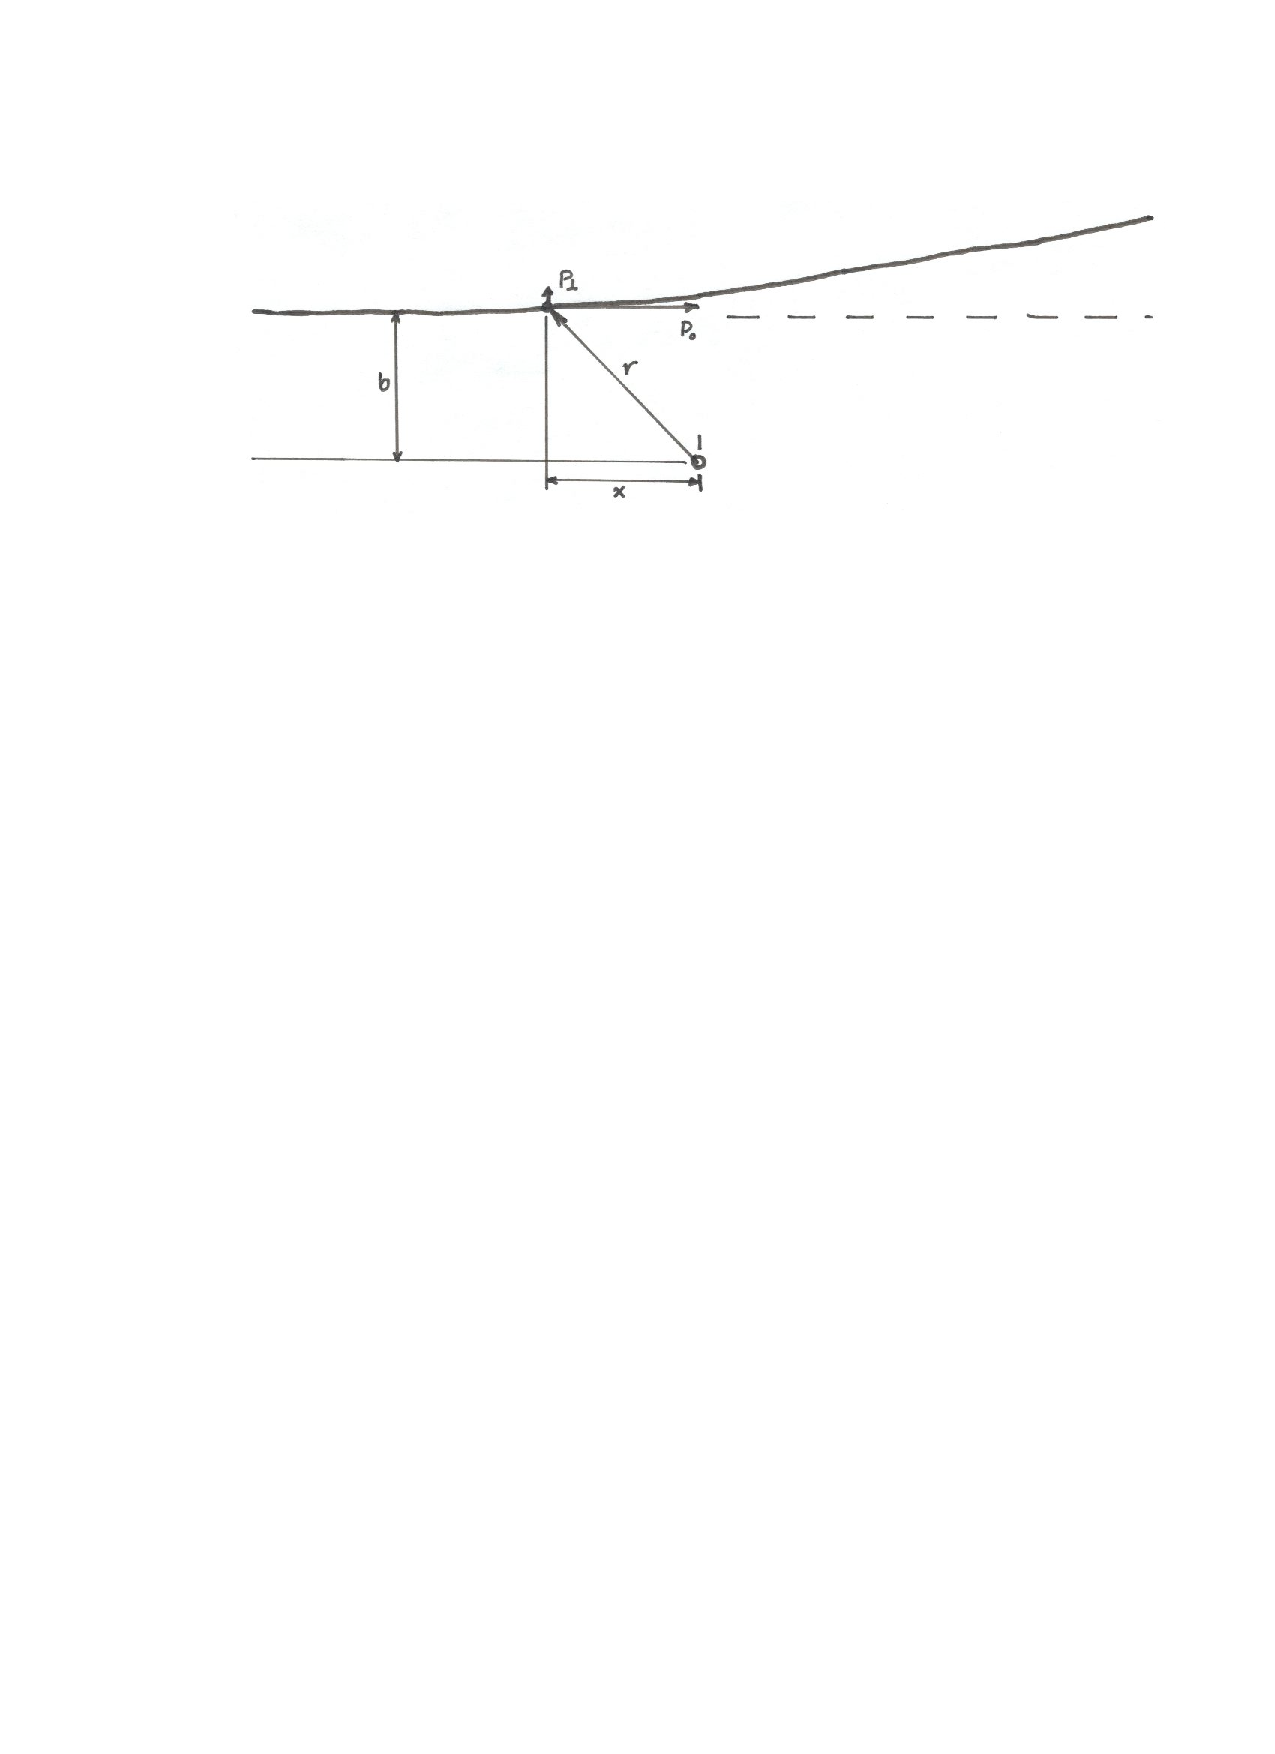
\includegraphics[width=\textwidth]{scattering}
\caption{Geometry for scattering problem.}
\label{f.scattering}
\end{figure}

As mentioned earlier, we are in a weakly coupled plasma, so we expect large angle scatterings to be a rare occurrence. What happens instead is that the particle suffers a number of small deflections. Let's consider an impact parameter in the range $(b,b+\dif b)$. Each deflection will have $\bvec{\Delta p}_{\bot}$ in some random direction, so
\[ \langle \bvec{ p}_{\bot}\rangle = \sum_{i=1}^{N} \bvec{\Delta p}_{i} \approx \bvec{0}. \]
What is happening is that the component of momentum perpendicular to $p_{0}$ is executing a random walk.  Indeed, after $N$ collisions,
\begin{eqnarray*} \langle \bvec{p}_{\bot} \vdot \bvec{p}_{\bot} \rangle  &=& \left( \sum_{i=1}^{N} \bvec{\Delta p}_{i}\right)\vdot \left( \sum_{i=1}^{N} \bvec{\Delta p}_{i} \right) \\
&=& \sum_{i=1}^{N} (\Delta p_{i})^{2} + 2\sum_{i\ne j} \bvec{\Delta p}_{i}\vdot\bvec{\Delta p}_{j} = N(\Delta p_{\bot})^{2},
\end{eqnarray*}
where we have assumed that all $\bvec{\Delta p}_{\perp}$ have the same magnitude and are uncorrelated. Now $N$ is just $\Delta t \times n \times (2\pi b \,\dif b) \times (p_{0}/\mu)$: the number of particles with impact parameters between $b$ and $b+\dif b$ along the length of the particles path over a time $\Delta t$.  Dividing by $\Delta t$ and integrating over $b$, we have the rate of change of the perpendicular component of the momentum
\begin{equation}\label{e.msdev-momentum}
\frac{\dif \langle p_{\bot}^{2}\rangle }{\dif t} = \frac{8\pi n\mu (q_{1}q_{2})^{2}}{p_{0}^{3}}\int_{b_{\mathrm{min}}}^{b_{\mathrm{max}}}\;\frac{\dif b}{b}.
\end{equation}
What are $b_{\mathrm{max}}$ and $b_{\mathrm{min}}$, the maximum and minimum impact parameters? Clearly, if $b > \lambda_{\mathrm{D}}$ then the potential will be screened.  Since our approximation is only good for $b > b_{0}$, we may take $b_{\mathrm{min}} = b_{0}$. (Our rate of scattering only depends logarithmically on $b_{\mathrm{max}}/b_{\mathrm{min}}$, so these estimates are good enough for our purposes).  With this substitution,
\begin{eqnarray}
\frac{\dif \langle p_{\bot}^{2}\rangle }{\dif t} &=& \frac{8\pi n\mu (q_{1}q_{2})^{2}}{p_{0}^{3}}\ln\left(\frac{\lambda_{\mathrm{D}}}{b_{0}}\right)\nonumber \\
 &\equiv& \frac{8\pi n\mu (q_{1}q_{2})^{2}}{p_{0}^{3}}\ln\Lambda.
\label{e.deflection-rate}
\end{eqnarray}
In the literature, the quantity $\ln\Lambda$ is called the Coulomb logarithm; for a plasma such as we are considering it is $\sim \ln  \left(\Lambda_{\mathrm{D}}^{3} n\right)$, the logarithm of the number of particles in a Debye sphere (see eq.~[\ref{e.plasma-parameter}]).  For conditions typical of the solar center (hydrogen plasma, $\rho \gtrsim 1\nsp\grampercc$, $T \approx 10^{7}\nsp\K$), $\ln\Lambda \approx \left(5\textrm{--}10\right)$.  

For small-angle scattering, the concept of a collision rate is fuzzy: the particle is constantly being bombarded by many tiny collisions.  Setting $\dif \langle p_{\bot}^{2}\rangle/\dif t = p_{0}^{2}$ allows us to define a deflection rate,
\begin{eqnarray}\label{e.scattering-rate}
\nu &\approx& \frac{8\pi n \mu (q_{1}q_{2})^{2}}{p_{0}^{3}} \ln\Lambda\\
 &=& \frac{8\pi n (q_{1}q_{2})^{2}}{(3\kB T)^{3/2}\mu^{1/2}}\ln\Lambda.
\end{eqnarray}
Comparing equations~(\ref{e.scattering-rate}) and (\ref{e.large-angle-collision-rate}), we see that many small angle scatterings are more important than single large angle scattering. Note that the ion-ion collision rate will be about $\sqrt{m_{p}/m_{e}} \approx 43$ times less than the electron-electron collision rate for a given temperature.

One can define a mean free path $\ell$ from equation~(\ref{e.scattering-rate}). Consider a particle incident on a cylinder of cross-sectional area $\mathcal{A}$ and length $\ell$, as illustrated in Figure~\ref{f.mfp}. We chose $\ell$ so that the time for the particle to traverse it is $\nu^{-1}$, the timescale for deflection.  Thus $\ell = v_{0}/\nu = p_{0}/(\mu\nu)$. Note that for a large angle collision, we can write the probability for scattering as the total cross-section of scatterers per unit area,
\begin{equation}\label{e.mfp-simple}
\mathcal{P} = \frac{N\sigma}{\mathcal{A}} = \frac{n\times(\ell\mathcal{A})\sigma}{\mathcal{A}},
\end{equation}
so the particle will suffer on average a collision after traversing a distance $\ell = (n\sigma)^{-1}$. Comparing equation~(\ref{e.mfp-simple}) with our expression for $\ell$ in terms of $\nu$ allows us to define an effective cross-section for small angle scattering.

\begin{figure}[htbp]
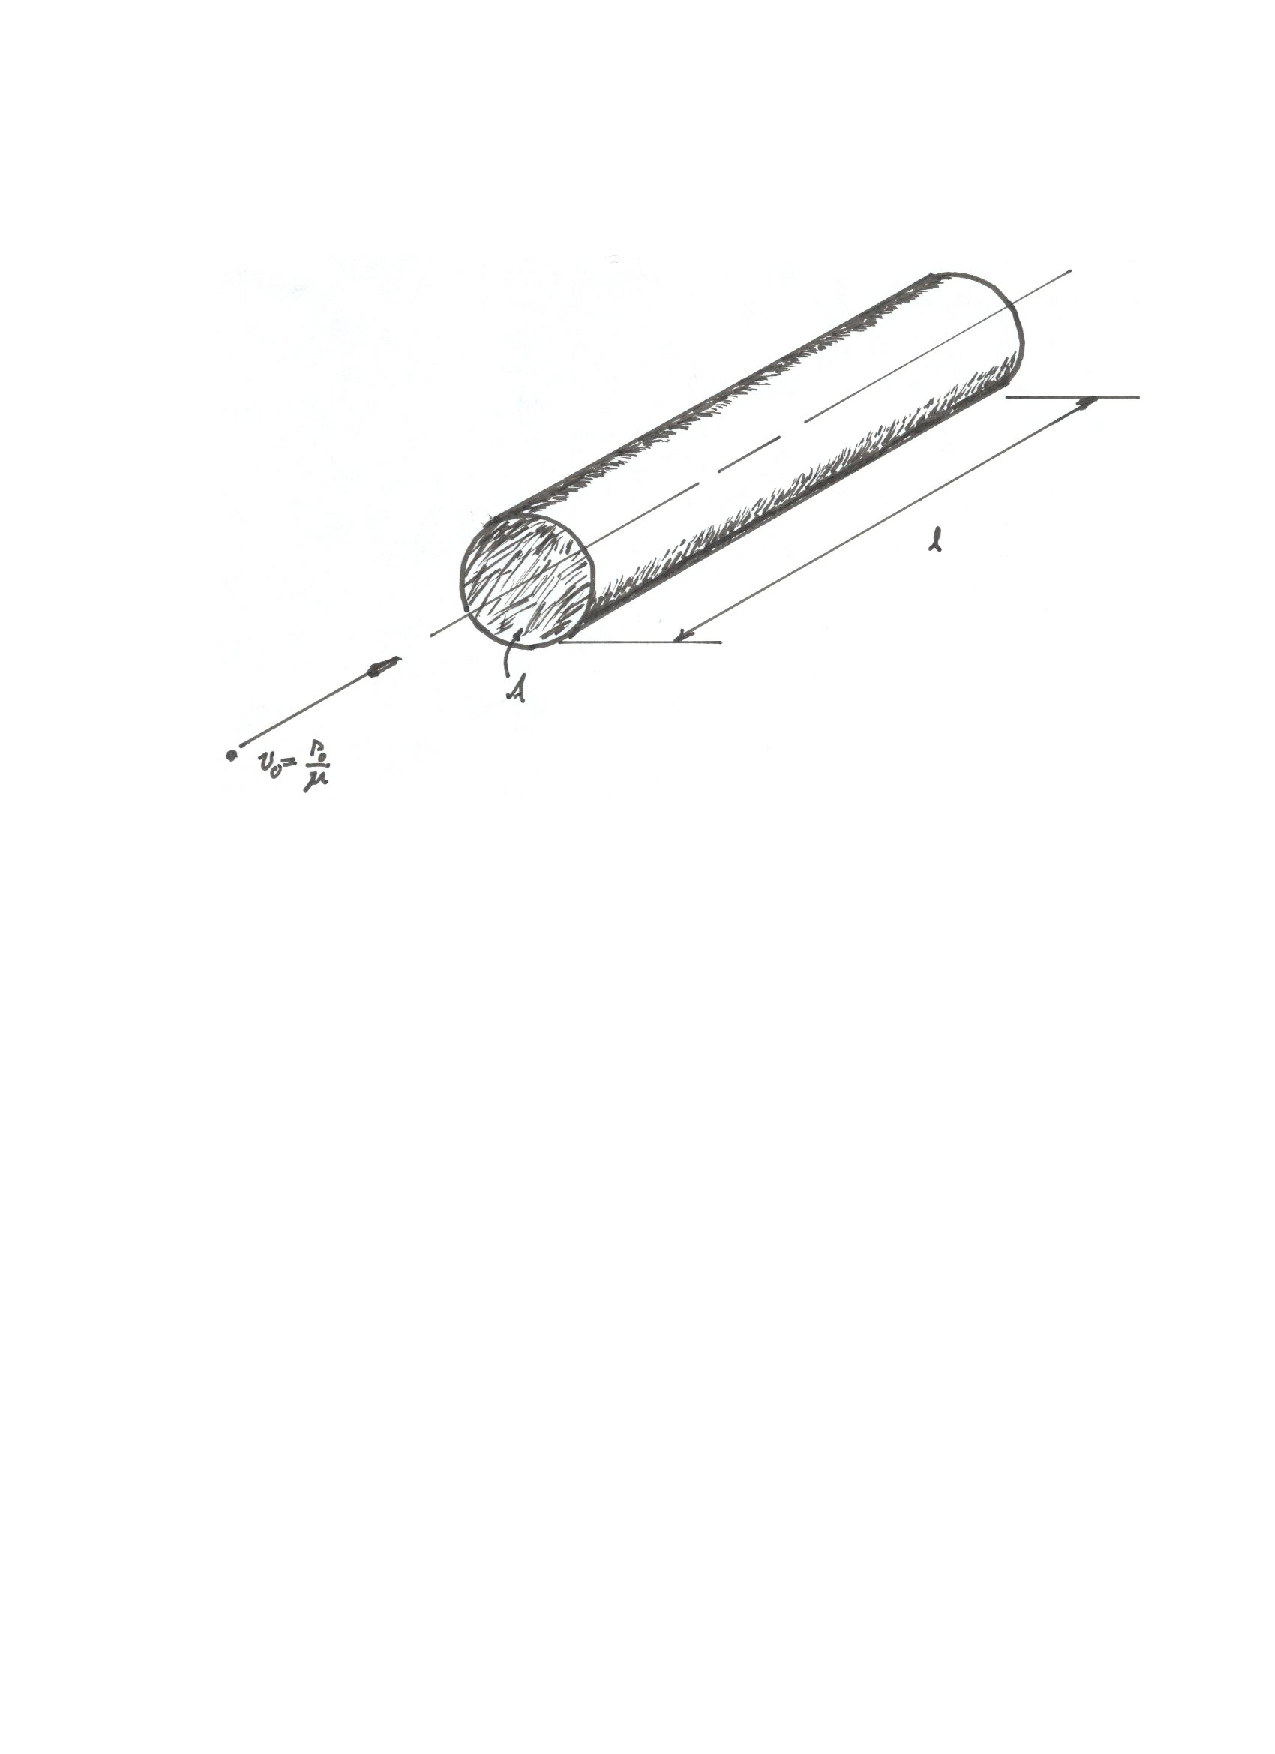
\includegraphics[width=\textwidth]{mean-free-path}
\caption{Schematic of a particle incident on a cylinder containing $n\times\ell\times\mathcal{A}$ particles.}
\label{f.mfp}
\end{figure}

\section{Transport properties}

We now have enough machinery to make estimates of \emph{transport coefficients,} such as the viscosity and the thermal conductivity. Let's begin with the viscosity.  Suppose we have a fluid with a gradient in the velocity, a shear, as depicted in Figure~\ref{f.shear-diagram}.  Let the mean thermal velocity of a particle be $v_{0}$.  In a time $\Delta t$, a number of particles will enter the box from the top, $(1/6) n v_{0} \Delta t$, and a similar number will leave the box via the top face. On average, these particles are endowed with the fluid properties of their last scattering, so the \emph{net} momentum carried into the box across the top face is
\begin{equation}\label{e.viscosity-1}
 \frac{1}{6} n m v_{0} \Delta t \Delta A \left[v_{y}(z_{t} + \ell) - v_{y}(z_{t}-\ell)\right] \approx \frac{1}{3} n m v_{0} \Delta t\Delta A \left.\frac{\partial v_{y}}{\partial z}\right|_{z_{t}}\ell.
\end{equation}
Here $\Delta A$ is the cross-section area of our box in the $xy$ plane and $z_{t}$ is the coordinate of the top face.

\begin{figure}[htbp]
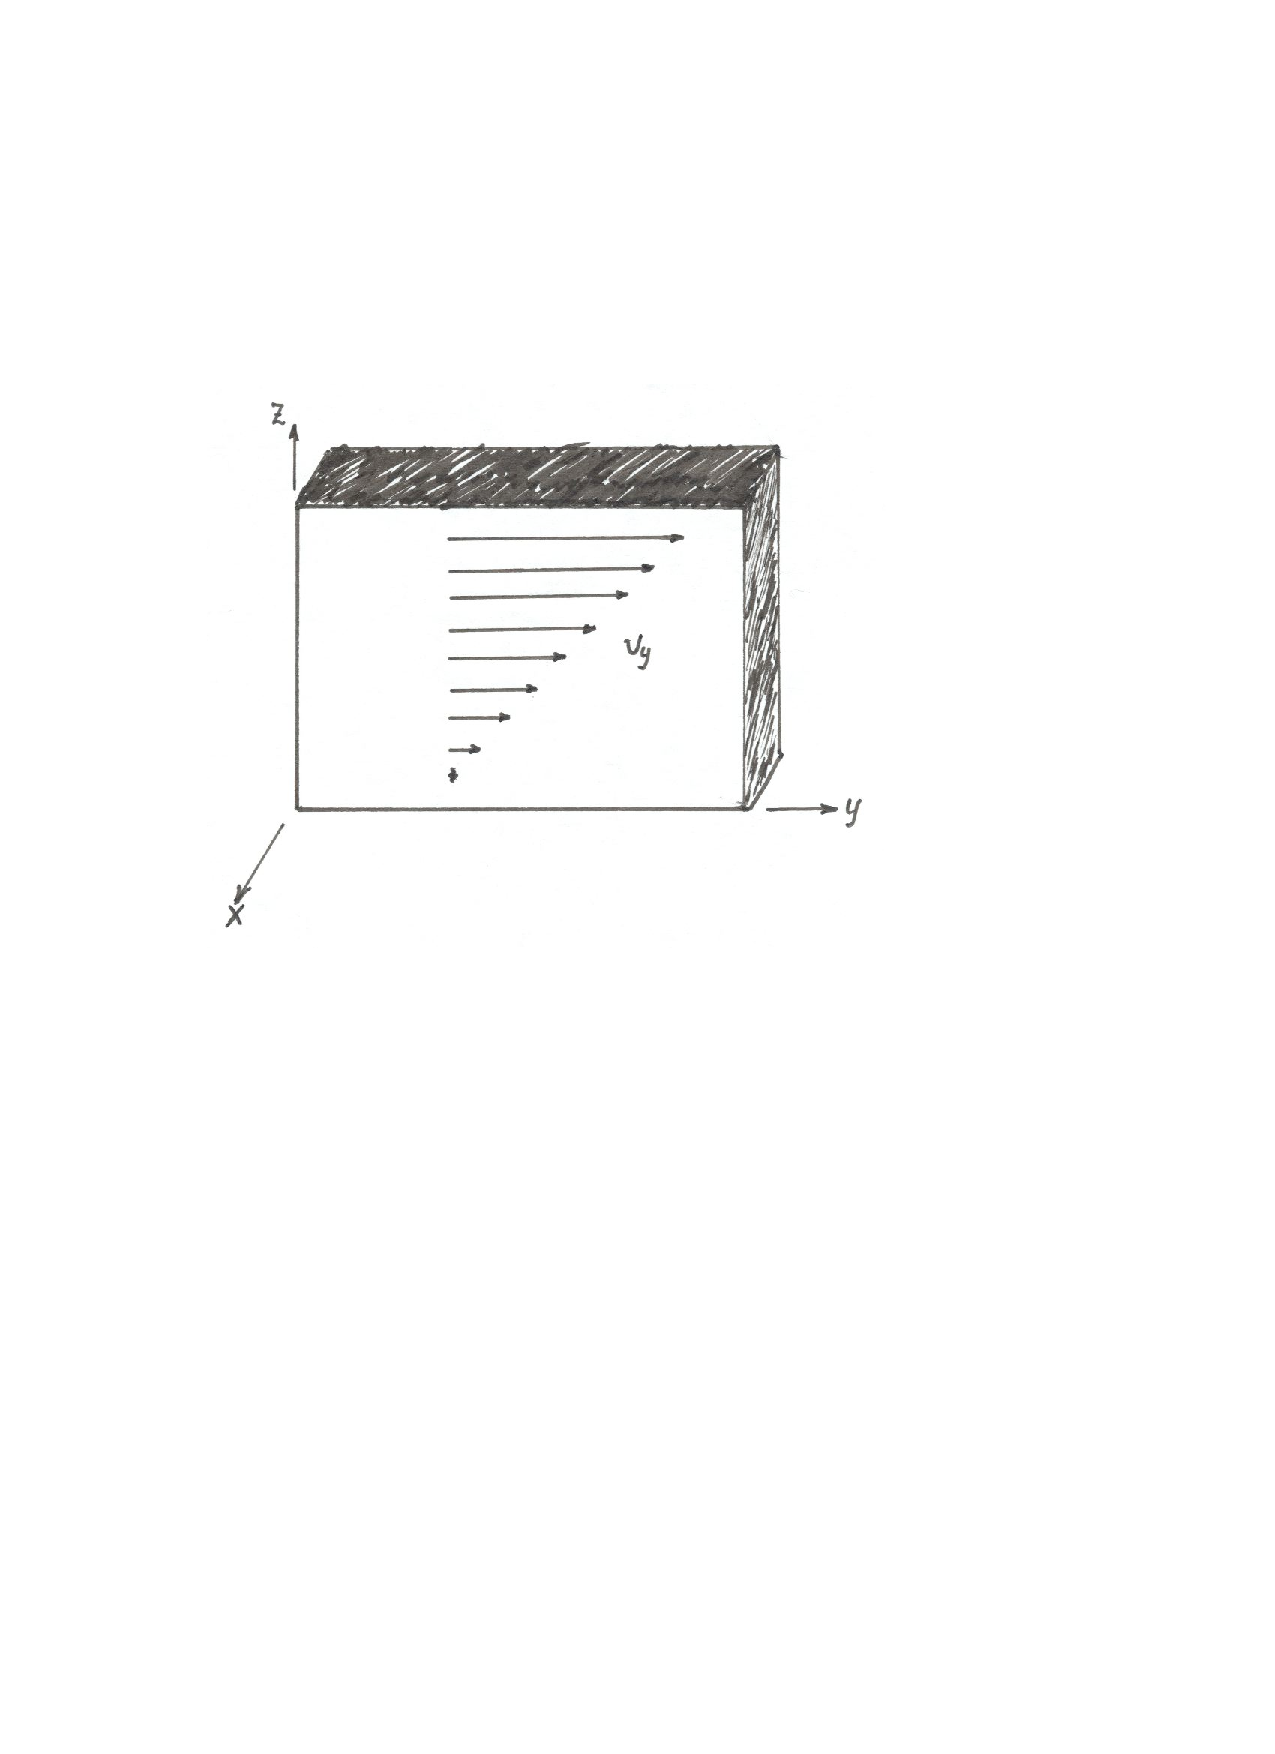
\includegraphics[width=\textwidth]{shear-diagram}
\caption{An element of fluid with a shear $\partial v_{y}/\partial z$.}\label{f.shear-diagram}
\end{figure}

A similar process occurs across the bottom face, located at coordinate $z=z_{b}$: the momentum flux across the bottom face is
\begin{equation}\label{e.viscosity-2} 
\approx -\frac{1}{3} n m v_{0} \Delta t\Delta A \left.\frac{\partial v_{y}}{\partial z}\right|_{z_{b}}\ell.
\end{equation}
Note the difference in sign: the momentum flux is positive if the $y$-velocity is larger below the box.  Putting equations~(\ref{e.viscosity-1}) and (\ref{e.viscosity-2}) together, the net change of momentum per time per unit volume $\Delta A\Delta z$ is
\begin{eqnarray}
\frac{1}{\Delta A\Delta z}\frac{\Delta p}{\Delta t} &\approx&  \frac{1}{\Delta z} \frac{1}{3} \left[\left(n m v_{0}\ell\frac{\partial v_{y}}{\partial z}\right)_{z_{t}} - \left(n m v_{0} \ell\frac{\partial v_{y}}{\partial z}\right)_{z_{b}}\right]\nonumber\\
 &\approx&   \frac{\partial}{\partial z}\left( \mu \frac{\partial v_{y}}{\partial z}\right).
\label{e.viscosity-3}
\end{eqnarray}
Here we have defined $\mu = nmv_{0}\ell/3 $ as the coefficient of dynamic viscosity. 

Dividing equation~(\ref{e.viscosity-3}) by the mass density modifies Euler's equation, eq.~(\ref{e.euler}), to the \emph{Navier-Stokes equation},
\begin{equation}\label{e.navier-stokes}
\partial_{t}\vu + \vu\cdot\grad\vu = -\grad \Phi - \frac{1}{\rho}\grad P + \frac{1}{\rho}\divr(\mu \grad\vu).
\end{equation}
In an isothermal, incompressible fluid, one can pull $\mu$ outside the divergence operator and the last term becomes
\[ \frac{\mu}{\rho}\nabla^{2}\vu \equiv \nu \nabla^{2}\vu, \]
where $\nu$ is defined as the \emph{coefficient of kinematic viscosity}. Note that in order-of-magnitude
\[ \nu \sim \frac{1}{3}v_{0}\ell,\]
that is, it is roughly the thermal velocity times the mean free path.

An identical proceedure, but replacing the average momentum of a particle with its average thermal energy, yields an expression for the \emph{thermal conductivity} $K$, such that the heat flux is
\begin{equation}\label{e.flux-equation}
\bvec{F} = -K\grad T.
\end{equation}
If one writes the change in energy of a fluid element as being 
\[\rho C \partial_{t}T = \divr(K\grad T),\]
 it can be seen that in order of magnitude the thermal diffusivity $\chi \equiv K/(\rho C)$, where $C$ is the specific heat per unit mass, is $\chi \sim (1/3) v_{0} \ell$.  (From the form of the equation and dimensional analysis, it has to be like this.)  But we need to be careful here: in a plasma with ions and electrons, the ions are responsible for momentum transport, whereas electrons, being more nimble, are more effective at heat transport.  Thus the thermal diffusivity is larger than the kinematic viscosity by a factor $\sim \sqrt{m_{p}/m_{e}}\approx 43$.

\section{Exercises}\label{s.plasma-exercises}
\begin{enumerate}
\item Show that equation~(\ref{e.plasma-parameter}) is equivalent to $\Gamma \ll 1$ for a single species plasma.

\item Show that for a non-relativistic plasma, the magnetic interaction between two charged particles is much less than the electrostatic interaction.

\item Show that the net charge in the shielding cloud about an ion of charge $Ze$ is $-Ze$; the shielding cloud cancels out the ion's charge.

\item Consider a fully ionized hydrogen plasma in a gravitational field in planar geometry. By adding the external potentials to the chemical potential, derive expressions for $\dif P_{e}/\dif z$ and $\dif P_{p}/\dif z$, the pressure gradients of electrons and protons, respectively.  
\begin{enumerate}
\item Argue that in the absence of an electric field, the protons would sink to the bottom of the atmosphere. Show that if the atmosphere is to remain charge neutral, then an electric field
\[
	\bvec{E} = -\frac{1}{2}\frac{\mb}{e}\bvec{g},
\]
must be present. Compare this field to that between the proton and electron in an atom.  Could this external field be detectable, by Stark effect for example?

\item Suppose a trace ion of charge $Z'e$ and mass $A'\mb$ is	 introduced.  What is the net force on this ion?

\item In order to have an electric field, there must be some charge separation.  Quantify this: define a parameter
\[ \delta \equiv \frac{n_{e}-n_{p}}{n_{e} + n_{p}} \]
and estimate its magnitude.  \emph{Hint:} Use Poisson's equation for both the gravitational and electrostatic potentials, and assume that $n_{e} = n_{p}$ to lowest order.

\end{enumerate}
\item 
\begin{enumerate} 
\item\label{p.zero-pressure-iron} In the zero-temperature limit (electrons are fully degenerate) use the charge-neutral sphere approximation (p.~\pageref{e.madelung-total}) to calculate the density at which completely ionized \iron[56] has zero pressure.

\item Estimate the pressure that would be required to compress \iron[56] at the density found in part~\ref{p.zero-pressure-iron}.
\end{enumerate}

\item Now write the total pressure as the sum of electron and Coulomb pressure, and use the virial scalings that we derived for pressure and density in terms of mass and radius, to obtain a relation between mass and radius for a cold object (``a rock'').  Find the mass having the largest radius, and express this mass in terms of fundamental physical constants.  How does it compare with the mass of Jupiter?  Scale the mass and radii to that of Jupiter, and plot $R(M)$ for pure \hydrogen, pure \helium, and pure \carbon\ objects.  Also indicate on this plot the masses and radii of the Jovian planets for comparison.

\item Estimate the ratio of the gravitational to viscous accelerations,
\[ \frac{|\grad\Phi|}{|\nu\nabla^{2}\vu|} ,\]
in equation~(\ref{e.navier-stokes}).  Express your answer in terms of a characteristic lengthscale, Mach number, and mean free path.  Under what conditions are viscous effects important?

\item Estimate the plasma thermal conductivity under conditions appropriate to the solar center.

\end{enumerate}

% !TEX root = ./notes.tex
\chapter[Stellar Atmospheres]{Stellar Atmospheres}

In the atmosphere of the star, the optical depth approaches unity, and we can no longer treat the radiation field as being isotropic. Let's consider the time-independent problem ($\partial_{t}\to 0$) of a plane-parallel atmosphere. The \emph{optical depth} for an outward-directed ray is
\begin{equation}\label{e.optical-depth}
\tau_{\nu} = \int _{z}^{\infty}\!\rho\kappa_{\nu}\,\dif z'.
\end{equation}
Now the optical depth just the distance divided by the mean free path. Clearly, when $\tau_{\nu} < 1$, a photon has a good chance of reaching a distant observer without any further interactions with the stellar matter.  As a result, the intensity takes its final form around $\tau_{\nu} \approx 1$, and this defines the stellar \emph{photosphere}. To get some of the basic properties of the photosphere, rewrite eq.~(\ref{e.optical-depth}) in differential form,
\begin{equation}\label{e.dtaudz}
\frac{\dif\tau}{\dif z} = -\rho\kappa.
\end{equation}
This is for a crude estimate, so we neglect the frequency dependence for now.  We can use equation~(\ref{e.dtaudz}) along with hydrostatic balance to get an estimate of the photospheric pressure,
\begin{equation}\label{e.photo-pressure}
\frac{\dif P}{\dif \tau} = -\left(\frac{\dif \tau}{\dif z}\right)^{-1}\rho g = \frac{g}{\kappa}.
\end{equation}
Thus, at $\tau \approx 1$, the pressure is $P_{\mathrm{ph}}\approx g/\kappa$. Since the flux at the photosphere is $\ssb \Teff^{4}$, we would expect that the local temperature is $T\approx \Teff$.

\section{The Eddington Approximation}

To get an analytical approximation for the atmosphere, we'll first redefine our transfer equation in terms of optical depth (eq.~[\ref{e.transfer-with-source}]). Here however, we will take the optical depth to be along the $z$-direction, so we define $\mu = \unitk\cdot\unitn$, where \unitn\ is the direction along the ray. The equation of transfer then becomes
\begin{equation}\label{e.planar}
\mu\frac{\partial I_{\nu}}{\partial\tau_{\nu}} = I_{\nu}-S_{\nu},
\end{equation}
where 
\begin{equation}\label{e.source}
S_{\nu} \equiv \frac{1}{\kappa_{\nu}}\left(\frac{\varepsilon_{\nu}}{4\pi} + \kappa_{\nu}^{\mathrm{sca}}J_{\nu}\right)
\end{equation}
is the \emph{source function}. In local thermodynamical equilibrium (LTE), we can write $S_{\nu} = (1-A_{\nu})B_{\nu} + A_{\nu}J_{\nu}$, where $A_{\nu} \equiv \kappa_{\nu}^{\mathrm{sca}}/\kappa_{\nu}$ is the \emph{albedo}.  Recall that $J_{\nu} = (4\pi)^{-1}\int\dif\Omega\,I_{\nu}$ is the angle-average of $I_{\nu}$.

We noted that in thermal equilibrium, $P_{\nu} = c^{-1}\int_{-1}^{1}\dif\mu\,\mu^{2}I_{\nu} = u_{\nu}/3$. This relation holds even when the radiation is not thermal, so long as it is isotropic to terms linear in $\mu$.  To make this concrete, suppose we write
\[ I_{\nu}(\mu) = I_{\nu}^{(0)} + \mu I_{\nu}^{(1)} + \mu^{2}I_{\nu}^{(2)} + \ldots. \]
Here we are assuming that terms marked $(0)$ are much larger than terms marked $(1)$, etc.  To lowest order, the energy density, flux, and momentum flux are then
\begin{eqnarray*}
u_{\nu} &=& \frac{2\pi}{c}\int_{-1}^{1}\dif\mu\,I_{\nu}(\mu) = \frac{4\pi}{c} I_{\nu}^{(0)},\\
F_{\nu} &=& 2\pi\int_{-1}^{1}\dif\mu\,\mu\,I_{\nu}(\mu) = \frac{4\pi}{3} I_{\nu}^{(1)},\\
P_{\nu} &=& \frac{2\pi}{c}\int_{-1}^{1}\dif\mu\,\mu^{2}\,I_{\nu}(\mu) = \frac{4\pi}{3c}I_{\nu}^{(0)} = \frac{u_{\nu}}{3}.
\end{eqnarray*}
The \emph{Eddington approximation} then consists of treating the radiation field as if its anisotropy is linear in $\mu$ \emph{everywhere}, so that the above relations hold; in particular, it means assuming that $P_{\nu} = u_{\nu}/3$ everywhere.

\section[Grey Atmosphere]{A Grey Atmosphere}

Finally, to get an analytical approximation to the structure of the solar atmosphere, let's consider a grey atmosphere in LTE, i. e., one for which $\kappa_{\nu}^{\mathrm{abs}} = \kappa^{\mathrm{abs}}$ and $\kappa_{\nu}^{\mathrm{sca}} = \kappa^{\mathrm{sca}}$ are independent of frequency. Equation~(\ref{e.planar}) can then be integrated over all frequencies to become
\begin{equation}\label{e.J-grey}
\mu\frac{\partial I}{\partial\tau} = I-S.
\end{equation}
Integrating over all angles (note that we can pull the derivative wrt $\tau$ out of the integral) gives
\begin{equation}\label{e.H-grey}
\frac{1}{4\pi}\frac{\partial F}{\partial\tau} = J - S = 0.
\end{equation}
Why does the right-hand side vanish? Note that $S-J = (1-A)(B-J)$.  Clearly $S = J$ if $A = 1$ (a pure scattering atmosphere).  If $A \ne 1$, so that there is some absorption, then the condition of detailed balance, equation~(\ref{e.detail-balance}), implies that $\varepsilon_{\nu} = 4\pi\kappa^{\mathrm{abs}}B_{\nu}(T)$; inserting this into equation~(\ref{e.rad-equil}), factoring out the constant $\kappa^{\mathrm{abs}}$, and integrating over $\nu$ implies that $B - J = 0$, and hence $S - J = 0$. Note that $J = B$ does \emph{not} necessarily imply that $I_{\nu} = B_{\nu}$!

Now multiply equation~(\ref{e.J-grey}) by $\mu$ and integrate over $2\pi\,\dif\mu$ to obtain
\begin{equation}\label{e.K-grey}
c\frac{\partial P}{\partial\tau} = F,
\end{equation}
the integral over $\mu S$ vanishing because it is odd in $\mu$. Equation~(\ref{e.H-grey}) implies that $F$ is constant; hence we can integrate equation~(\ref{e.K-grey}) at once to obtain
\begin{equation}\label{e.KH}
cP = F(\tau + \tau_{0}),
\end{equation}
where $\tau_{0}$ is a constant of integration. Of course, this does help us yet; all we have done is introduce a new variable $P$, the radiation pressure. This is where the Eddington approximation comes in.  We set $P = u/3 = 4\pi J/(3c)$ in equation~(\ref{e.KH}) to obtain $4\pi J = 3F(\tau + \tau_{0})$. Since $J = S$, we can then write equation~(\ref{e.J-grey}) as
\begin{equation}
\mu\frac{\partial I}{\partial\tau} = I - \frac{3}{4\pi}F(\tau+\tau_{0}).
\end{equation}
Since $F$ is constant, this first-order differential equation is now solvable,
\begin{eqnarray}
I(\mu,\tau=0) &=& \frac{1}{\mu}\int_{0}^{\infty}\!\frac{3}{4\pi}F(\tau + \tau_{0}) e^{-\tau/\mu}\,\dif\tau,\nonumber\\
  &=& \frac{3}{4\pi}F(\mu + \tau_{0}).\label{e.I-Edd}
\end{eqnarray}
Now at $\tau = 0$, all of the flux must be outward-directed ($\mu >0$), so $I(\mu < 0,\tau = 0) = 0$ if the star is not irradiated by another source.  Note that the Eddington approximation is clearly violated here.  Still, we will see later that this approximation is not too terrible. 

To determine $\tau_{0}$, multiply $I(\mu,\tau = 0)$ by $\mu$ and integrate equation~(\ref{e.I-Edd}) over all angles to find
\begin{equation}
F = 2\pi\int_{0}^{1}\!\mu I(\mu,0)\,\dif\mu = \frac{1}{2}\int_{0}^{1}\!3F(\mu + \tau_{0})\,\mu\,\dif\mu = F\left(\frac{1}{2} + \frac{3}{4}\tau_{0}\right).
\end{equation}
We therefore find $\tau_{0} = 2/3$. Now, since we are in LTE, $P = aT^{4}/3$. Further, let us define an effective temperature by the relation $F = \ssb\Teff^{4}$.  Substituting these definitions and the value of $\tau_{0}$ into equation~(\ref{e.KH}) gives us the atmospheric temperature structure,
\begin{equation}\label{e.Eddington}
T^{4}(\tau) = \frac{3}{4}\Teff^{4}\left(\tau + \frac{2}{3}\right).
\end{equation}
Thus $T(\tau  = 0) = 2^{-1/4} \Teff$ and $T(\tau = 2/3) = \Teff$.  To get the spectral distribution, go back to equation~(\ref{e.planar}) and (assuming the atmosphere has some absorption so that the matter and radiation can come into equilibrium) insert $S_{\nu} = B_{\nu}(T)$; solving for $I_{\nu}$ at $\tau = 0$ then gives
\begin{equation}\label{e.spectral}
I_{\nu}(\mu,\tau=0) = \frac{1}{\mu}\int_{0}^{\infty}\!B_{\nu}\left[T(\tau)\right] \, e^{-\tau/\mu}\,\dif\tau.
\end{equation}
A plot of the spectral distribution for the emergent flux is shown (\emph{open circles}) in Fig.~\ref{f.spectral}. For comparison, a plot of the Planck distribution (\emph{solid line}) is also shown. Both fluxes are normalized to the total flux.  Note that $I_{\nu}(\mu,\tau=0)$ depends on angle; rays propagating at a slant will have a lower intensity.  As a result, when we observe the sun, the edge of the visible disk appears darker than the center, a phenomenon known as \emph{limb darkening}.

\begin{figure}[htbp]
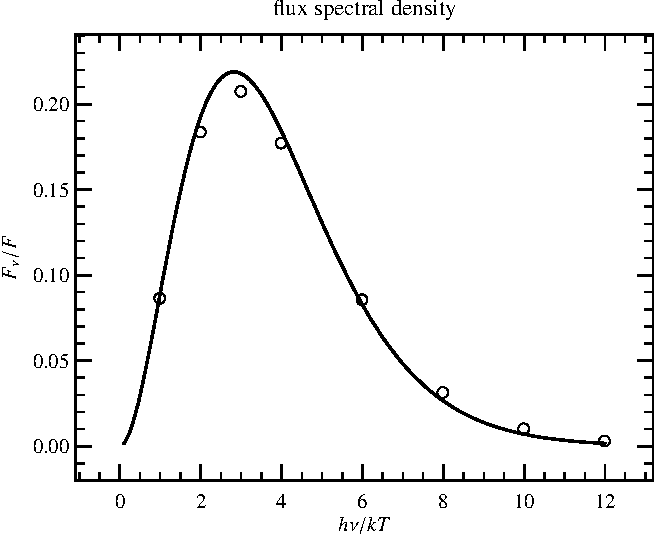
\includegraphics[width=4in]{plots_out/spectral_distribution}
\caption{\label{f.spectral} Spectral distribution from a grey atmosphere. The open circles are from Chandrasekhar, \emph{Radiative Transfer}; the solid line is the Planck distribution.}
\end{figure}

\section{Some applications}

\subsection{Requirement for convection in the atmosphere}\label{s.atmosphere-convection}

Let's construct a simple atmosphere model using our temperature structure, eq.~(\ref{e.Eddington}).  Although we assume a grey opacity, we will let if vary with temperature and density, $\kappa(\rho,T) = \kappa_{0}\rho^{r}T^{s}$.  For an ideal gas, we can rewrite this in terms of pressure and temperature, $\kappa(P,T) = \kappa_{0} (\mu\mb/k)^{r}P^{r} T^{s-r}$.  Substituting this into equation~(\ref{e.photo-pressure}), and using equation~(\ref{e.Eddington}), we obtain,
\[
  \frac{\dif P}{\dif \tau} = \frac{g}{\kappa_{0}}\left(\frac{k}{\mu\mb}\right)^{r} P^{-r} \left[\frac{3}{4}\Teff^{4}\left(\tau + \frac{2}{3}\right)\right]^{(r-s)/4}.
\]
This is easily integrated: we'll take $P(\tau = 0) = 0$ and obtain
\[
  P(\tau) = (\mathrm{const})\tau^{(r-s+4)/4/(1+r)}
\]
so that
\begin{equation}\label{e.dlnPdtau}
  \frac{\dif \ln P}{\dif \tau} = \frac{r-s+4}{4(1+r)\tau}.
\end{equation}
For the temperature,
\begin{equation}\label{e.dlnTdtau}
 \frac{\dif\ln T}{\dif\tau} = \frac{1}{4}\frac{\dif\ln T^{4}}{\dif \tau} = \frac{1}{4(\tau + 2/3)}.
\end{equation}
We now combine eqn.~(\ref{e.dlnPdtau}) and (\ref{e.dlnTdtau}) to obtain
\begin{equation}\label{e.dlnTdlnP-atmosphere}
\frac{\dif \ln T}{\dif\ln P} = \left(\frac{1+r}{r-s +4}\right)\left(\frac{\tau}{\tau + 2/3}\right).
\end{equation}
For convection to happen, $\dif\ln T/\dif\ln P > (\partial\ln T/\partial\ln P)_{s} = 1/(1+n)$, where $n = 3/2$ for an ideal gas.  That is,
\begin{equation}\label{e.convection-will-happen}
 n > \frac{r-s + 4}{1+r} - 1 = \frac{3-s}{1+r},
\end{equation}
is required for convection to happen somewhere.  Table~\ref{t.rhs} illustrates the behavior of $\dif\ln T/\dif\ln P$ for various opacity sources.  The fact that the H$^{-}$ opacity increases with temperature forces the temperature gradient to steepen with increasing pressure and ensures that low-mass stars have outer convective zones.

\begin{table}[htbp]
\caption{Right-hand side of eq.~(\ref{e.convection-will-happen}) for various opacities}
\label{t.rhs}
\begin{center}
\begin{tabular}{lrrr}
\hline
source & $r$ & $s$ & $\frac{3-s}{1+r}$\\
\hline
Thomson & $0$ & $0$ & $3$\\
free-free & $14$ & $-7/2$ & $13/4$\\
H$^{-}$ & $1/2$ & $9$ & $-4$\\
\hline
\end{tabular}
\end{center}
\end{table}

\subsection{The Hayashi Track}\label{s.Hayashi}

For a fully convective star, we can use the fact that the entropy per unit mass is the same at the photosphere as at the center to relate the surface temperature to the mass and radius of the star. Namely,
\begin{equation}\label{e.Teff-adiabat}
\Teff = T_{c}\left(\frac{P_{\mathrm{ph}}}{P_{c}}\right)^{2/5},
\end{equation}
with
\begin{eqnarray}
T_{c} &=& 0.5 \frac{GM\mu \mb}{kR} \label{e.fc-Tc}\\
P_{c} &=& 0.8\frac{GM^{2}}{R^{4}} \label{e.fc-Pc}
\end{eqnarray}
being the central density and pressure of a polytrope of index $n=3/2$, and $P_{\mathrm{ph}}$ being the root of the equation
\begin{equation}\label{e.pph}
 P_{\mathrm{ph}} \approx \frac{GM}{R^{2}}\frac{1}{\kappa_{0}(\mu\mb/k)^{r}P_{\mathrm{ph}}^{r}\Teff^{s-r}}. 
\end{equation}
(We could have used the solution for $P(\tau)$ from before, but this approximation is accurate enough to demonstrate our point.)

Now for some crazy fractions: insert equations~(\ref{e.fc-Tc}), (\ref{e.fc-Pc}), and (\ref{e.pph}) into equation~(\ref{e.Teff-adiabat}) and solve for $\Teff$ to find
\begin{equation}\label{e.Teff-MR}
\Teff^{5+3r+2s} = 0.55^{5(1+r)}\kappa_{0}^{-2} \left(\frac{G\mu\mb}{k}\right)^{5+3r}M^{3+r} R^{3r-1}.
\end{equation}
What does this say for Thomson scattering ($\kappa_{0} \approx 0.4$, $r=s=0$)? Inserting these values into eq.~(\ref{e.Teff-MR}) gives
\begin{equation}\label{e.Teff-th}
	\Teff \approx 250\nsp\K \left(\frac{M}{\Msun}\right)^{3/5}\left(\frac{R}{R_{\odot}}\right)^{-1/5},
\end{equation}
a ridiculous value. Let's try it with H$^{-}$ opacity ($\kappa_{0} \approx 2.5\ee{-31}$, $r=1/2$, $s=9$). In this case,
\begin{equation}\label{e.Teff-H-}
 \Teff \approx 2200\nsp\K \left(\frac{M}{\Msun}\right)^{1/7}\left(\frac{R}{\Rsun}\right)^{1/49}.
\end{equation}
Note the extremely weak dependence on $R$.  This is a consequence that $R$ is very sensitive to the entropy at the photosphere.  Writing $L = 4\pi R^{2}\ssb \Teff^{4}$, we can solve for $R$ and insert it into equation~(\ref{e.Teff-H-}) to get the effective temperature in terms of mass and luminosity,
\begin{equation}\label{e.Hayashi}
 \Teff \approx 2300\nsp\K \left(\frac{M}{\Msun}\right)^{7/51}\left(\frac{L}{L_{\odot}}\right)^{1/102}.
\end{equation}
This is a crude estimate, so don't take these numbers too seriously. This exercise does illustrate, however, that the effective temperature for fully convective, low-mass stars is basically independent of luminosity.  On an HR diagram, these stars follow a vertical track, the \emph{Hayashi track} as they contract to the main sequence.

\subsection{The two-stream formalism, and an irradiated atmosphere}\label{s.two-stream}

Many extra-solar planets are in rather tight orbits and as a result are strongly irradiated.  The following example is a simplified treatment of \citet{Hummer1982The-effect-of-r} and \citet{Hubeny2003A-Possible-Bifu}. At a distance $D$ from the star, the luminous flux is $4\pi R_{\star}^{2}\ssb T_{\star}^{4}/(4\pi D^{2}) = \ssb T_{\star}^{4}(R_{\star}/D)^{2}$. The incident intensity is then $(\ssb/\pi)WT_{\star}^{4}$, where $W = (R_{\star}/D)^{2}$, since this will give the flux when integrated over all forward directions. 

An classic approximation in stellar atmospheres is to write the intensity as a sum of two streams,
\begin{equation}\label{e.two-stream}
I_{\nu}(\mu) = I_{\nu}^{+}\delta\left(\mu-\frac{1}{\sqrt{3}}\right) + I_{\nu}^{-}\delta\left(\mu + \frac{1}{\sqrt{3}}\right).
\end{equation}
The reason for the choice of $\mu$ becomes apparent when we compute the mean intensity, the flux, and the pressure:
\begin{eqnarray*}
J_{\nu} &=& \frac{1}{4\pi}\int\,\dif\phi\,\dif\mu I = \frac{1}{2}\left(I_{\nu}^{+} + I_{\nu}^{-}\right)\\
F_{\nu} &=& \int\,\dif\phi\,\dif\mu\;\mu I = \frac{2\pi}{\sqrt{3}} \left( I_{\nu}^{+} - I_{\nu}^{-}\right)\\
P_{\nu} &=& \frac{1}{c} \int\,\dif\phi\,\dif\mu\;\mu^{2} I = \frac{2\pi}{3c}\left(I_{\nu}^{+} + I_{\nu}^{-}\right).\\
\end{eqnarray*}
You will recognize by comparing $P_{\nu}$ with $J_{\nu}$ that this formalism automatically satisfies the Eddington approximation, since $J_{\nu} = (c/4\pi)u_{\nu}$.

With this approximation, we can take successive moments of our equation of transfer (for a grey atmosphere),
\[ \mu\frac{\dif I}{\dif \tau} = I-S, \]
to obtain
\begin{eqnarray}
\frac{\dif F}{\dif \tau} &=& 4\pi (J - S) \label{e.2streamF}\\
c\frac{\dif P}{\dif\tau} &=& F. \label{e.2streamP}
\end{eqnarray}
In LTE, $J - S = 0$ and therefore $F = \textrm{const}$.  We can therefore integrate eq.~(\ref{e.2streamP}), and use the Eddington approximation, $cP = (4\pi/3)J$, to obtain
\begin{equation}\label{e.2stream-1}
J(\tau) = \frac{3}{4\pi} F \tau + J_{0}.
\end{equation}
To fix $J_{0}$, we use our two stream approximation to write $J_{0} = (\sqrt{3}/4\pi)F + I^{-}$.  Since $F$ is constant, we can determine it by its value at great depth in the star.  Let us define a temperature $T_{\mathrm{int}}$ by the relation $F = \ssb T_{\mathrm{int}}^{4}$.  Finally, we set $I^{-}$ to the incident intensity, $I^{-} = (\ssb/\pi)WT_{\star}^{4}$ and note that in radiative equilibrium, $J = B = (\ssb/\pi) T^{4}(\tau)$. Collecting terms, we have the equation for the temperature structure,
\begin{equation}\label{e.T-irradiated}
T^{4}(\tau) = \frac{3}{4} T_{\mathrm{int}}^{4}\left(\tau + \frac{1}{\sqrt{3}}\right) + W T_{\star}^{4}.
\end{equation}
If $WT_{\star} \gg T_{\mathrm{int}}$, then the temperature is nearly isothermal to a depth $\tau_{h} \approx W(T_{\star}/T_{\mathrm{int}})^{4}$.
In general, the assumption of a grey atmosphere is quite poor: the incident photons are peaked in the optical, whereas the local temperatures are in the infrared, so that even taking a mean opacity is not sufficient.

\section{Line formation and the curve of growth}

A classical technique in the analysis of stellar spectra is to construct the \emph{curve of growth}, which relates the equivalent width of a line $W_{\nu}$ to the opacity in the line. This discussion follows Mihalas, \emph{Stellar Atmospheres}.

Let's first get the opacity in the line.  We saw in class that the cross-section for the transition $i\to j$ could be written as 
\begin{equation}\label{e.cross-section}
\sigma_{\nu} = \left(\frac{\pi e^{2}}{m_{e}c}\right)f_{ij}\phi_{\nu},
\end{equation}
where the first term is the classical oscillator cross-section, $f_{ij}$ is the oscillator strength and contains the quantum mechanical details of the interaction, and $\phi_{\nu}$ is the line profile.  Now recall that the opacity is given by $\kappa_{\nu} = n_{i}\sigma_{\nu}/\rho$, where $n_{i}$ denotes the number density of available atoms in state $i$ available to absorb a photon.  Furthermore, we need to allow for \emph{stimulated emission} from state $j$ to state $i$. With this added, the opacity is (I'm writing it as $\chi_{\nu}$ to distinguish it from the \emph{continuum opacity})
\begin{equation}\label{e.opacity}
\rho\chi_{\nu} = \left(\frac{\pi e^{2}}{m_{e}c}\right)f_{ij}\phi_{\nu}n_{i}\left[1 - \frac{g_{i}}{g_{j}}\frac{n_{j}}{n_{i}}\right].
\end{equation}
If we are in LTE, then the relative population of $n_{i}$ and $n_{j}$ follow a Boltzmann distribution,
\[ 1 - \frac{g_{i}}{g_{j}}\frac{n_{j}}{n_{i}} = 1- \exp\left(-\frac{h\nu}{kT}\right). \]
This ensures we have a positive opacity. If our population were inverted, i.~e., more atoms in the upper state $j$, then the opacity would be negative and we would have a \emph{laser}.

Now for the line profile.  In the case where we have doppler broadening and damping, the profile follows the \emph{Voigt} function,
\begin{equation}\label{e.voigt} \phi_{\nu} = \frac{1}{\Delta \nu_{D}}H(a,v), \end{equation}
where $\Delta\nu_{D} \equiv \nu u_{0}/c$ is the doppler width, with $u_{0}$ being the mean (thermal) velocity of the atoms, $a \equiv \Gamma/(4\pi\Delta\nu_{D})$ is the ratio of the damping width $\Gamma$ to the doppler width, and $v \equiv \Delta\nu/\Delta\nu_{D}$ is the difference in frequency from the line center in units of the doppler width.

Let's combine the line opacity with the continuum opacity and solve the equation of transfer.
For simplicity, we are going to assume pure absorption in both the continuum and the line.  Under these conditions, the source function is (see the notes on the Eddington atmosphere) $S_{\nu} = B_{\nu}$, the Planck function. For a plane-parallel atmosphere, the equation of transfer is then
\begin{equation}\label{e.cg-transfer}
\mu\frac{\dif I_{\nu}}{\dif\tau_{\nu}} = I_{\nu} - B_{\nu}
\end{equation}
where $\mu$ is the cosine of the angle of the ray with vertical. Solving equation~(\ref{e.cg-transfer}) for the emergent intensity at $\tau_{\nu} = 0$ gives
\begin{equation}\label{e.intensity}
I_{\nu}(\mu) = \frac{1}{\mu}\int_{0}^{\infty}\!B_{\nu}[T(\tau_{\nu})] \exp(-\tau_{\nu}/\mu) \,\dif\tau_{\nu}.
\end{equation}
The opacity is given by
\begin{equation}\label{e.total-opacity}
\kappa_{\nu} = \kappa_{\nu}^{C} + \chi_{\nu},
\end{equation}
where $\kappa_{\nu}^{C}$ is the continuum opacity and $\chi_{\nu} = \chi_{0}\phi_{\nu}$ is the line opacity, with 
\[
\chi_{0} = \frac{1}{\rho}\left(\frac{\pi e^{2}}{m_{e}c}\right)f_{ij}n_{i}\left(1 - e^{h\nu_{\ell}/kT}\right)
\]
being the line opacity at the line center $\nu_{\ell}$. 

As a further simplification, we can usually ignore the variation with $\nu$ in $\kappa_{\nu}^{C}$ over the width of the line. As a more suspect approximation (although it is not so bad in practice), let's assume that $\beta_{\nu} \equiv \chi_{\nu}/\kappa_{C}$ is independent of $\tau_{\nu}$. With this assumption we can write $\dif\tau_{\nu} = (1+\beta_{\nu})\dif\tau$, where $\tau = -\rho\kappa^{C}\,\dif z$. Finally, let's assume that in the line forming region, the temperature does not vary too much, so that we can expand $B_{\nu}$ to first order in $\tau$,
\[ B_{\nu}[T(\tau)] \approx B_{0} + B_{1}\tau, \]
where $B_{0}$ and $B_{1}$ are constants.
Inserting these approximations into equation~(\ref{e.intensity}), multiplying by the direction cosine $\mu$ and integrating over outward bound rays gives us the flux,
\begin{eqnarray}\label{e.flux}
F_{\nu} &=& 2\pi\int_{0}^{1}\!\int_{0}^{\infty}\!\left[B_{0}+B_{1}\tau\right]\exp\left[-\frac{\tau}{\mu}(1+\beta_{\nu})\right] \left(1+\beta_{\nu}\right) \,\dif\tau\,\dif\mu\nonumber\\
 &=& \pi\left[ B_{0} + \frac{2}{3}\frac{B_{1}}{1+\beta_{\nu}}\right].
\end{eqnarray}
Far from the line-center, $\beta_{\nu}\to 0$, implying that the continuum flux is
\[ F_{\nu}^{C} = \pi\left[B_{0} + \frac{2B_{1}}{3}\right]. \]
Hence the depth of the line is
\begin{equation}\label{e.line-depth}
A_{\nu} \equiv 1 - \frac{F_{\nu}}{F_{\nu}^{C}} = A_{0}\frac{\beta_{\nu}}{1+\beta_{\nu}},
\end{equation}
where
\begin{equation}\label{e.A0-curve-growth}
 A_{0} \equiv \frac{2B_{1}/3}{B_{0} + 2B_{1}/3}
 \end{equation}
is the depth of an infinitely opaque ($\beta_{\nu}\to\infty$) line. 

\noindent Now that we have the depth of the line $A_{\nu}$ we can compute the \emph{equivalent width},
\begin{equation}\label{e.W}
W_{\nu} \equiv \int_{0}^{\infty}\! A_{\nu}\,\dif\nu = A_{0}\int_{0}^{\infty}\!\frac{\beta_{\nu}}{1+\beta_{\nu}}\,\dif\nu.
\end{equation}
Let's change variables from $\nu$ to $v = \Delta\nu/\Delta\nu_{D} = (\nu-\nu_{\ell})/\Delta\nu_{D}$.  Since $H(a,v)$ is symmetrical about the line center, we will just integrate over $\Delta\nu >0$, giving
\begin{equation}\label{e.Wv}
 W_{\nu} = 2A_{0}\Delta\nu_{D}\int_{0}^{\infty}\!\frac{\beta_{0}H(a,v)}{1+\beta_{0}H(a,v)}\,\dif v,
 \end{equation}
with $\beta_{0} = \chi_{0}/(\kappa^{C}\Delta\nu_{D})$.

It's useful to understand the behavior of $W_{\nu}$ in various limits.  
First, at small line optical depth ($\beta_{0}\ll 1$) only the core of the line will be visible. Recall that in the core of the line, $H(a,v) \approx \exp(-v^{2})$ so we insert this into equation~(\ref{e.Wv}) and expand the denominator to give
\begin{eqnarray}\label{e.linear}
W_{\nu}^{\star} \equiv \frac{W{\nu}}{2A_{0}\Delta\nu_{D}} &=& \int_{0}^{\infty} \!\sum_{k=1}^{\infty}(-1)^{k-1}\beta_{0}^{k}e^{-kv^{2}}\,\dif v\nonumber\\
 &=& \frac{1}{2}\sqrt{\pi}\beta_{0}\left[1-\frac{\beta_{0}}{\sqrt{2}} + \frac{\beta_{0}^{2}}{\sqrt{3}} - \ldots\right].
\end{eqnarray}
Here $W_{\nu}^{\star}$ is the \emph{reduced equivalent width}.
Notice that since $\beta_{0}\propto 1/\Delta\nu_{D}$ (cf.~eq.~[\ref{e.voigt}]), the equivalent width $W_{\nu}$ is independent of $\Delta\nu_{D}$ in this \emph{linear regime}.
Physically, in the limit of small optical depth, each atom in state $i$ is able to absorb photons, and the flux removed  is just proportional to the number of atoms $n_{i}$.

As we increase $\beta_{0}$ eventually the core of the line saturates---no more absorption in the core is possible.  As a result, the equivalent width should be nearly constant until there are so many absorbers that the damping wings contribute to the removal of flux.  In the \emph{saturation regime}, the Voigt function is still given by $e^{-v^{2}}$, but we can no longer assume $\beta_{0}\ll 1$, so our expansion in equation~(\ref{e.linear}) won't work. Let's go back to our integral, eq.~(\ref{e.Wv}), change variables to $z= v^{2}$, and define $\alpha = \ln\beta_{0}$ to find
\[
W_{\nu}^{\star} = \frac{1}{2}\int_{0}^{\infty}\!\frac{z^{-1/2}}{e^{z-\alpha}+1}\,\dif z.
\]
This may not look like an improvement, but you might notice that it bears a resemblance to a Fermi-Dirac integral (see the notes on the equation of state). That means that very smart people figured out tricks to handle these integrals and all we have to do is look up what they did.  In this case we have Sommerfeld to thank. In this saturation regime,
\begin{equation}\label{e.saturation}
W_{\nu}^{\star} \approx \sqrt{\ln\beta_{0}}\left[ 1 - \frac{\pi^{2}}{24(\ln\beta_{0})^{2}} - \frac{7\pi^{4}}{384(\ln\beta_{0})^{4}}-\ldots\right].
\end{equation}
Note that the amount of flux removed is basically $2A_{0}\Delta\nu_{D}$: the line is maximally dark across the gaussian core.

Finally, if we continue to increase the line opacity, there will finally be so many absorbers that there will be significant flux removed from the wings.  Now the form of the Voigt profile is $H(a,v)\approx (a/\sqrt{\pi}) v^{-2}$, so our integral (eq.~[\ref{e.Wv}]) in this \emph{damping regime} becomes
\begin{eqnarray}\label{e.damping}
W_{\nu}^{\star} &=& \int_{0}^{\infty}\! \left(1+\frac{\sqrt{\pi}v^{2}}{\beta_{0}a}\right)^{-1}\, \dif v\nonumber\\
 &=& \frac{1}{2}\left(\pi a \beta_{0}\right)^{1/2}.
\end{eqnarray}
Note that since $a\beta_{0}\propto \Delta\nu_{D}^{-2}$, $W_{\nu}$ is again independent of the doppler width in this regime.

Now that we have this curve of growth, why is it useful? Since it only involves the equivalent width, it is possible to construct the curve of growth empirically without a high-resolution spectrum. Next, let's put some of the factors back into the quantities in the curve of growth.  First, for a set of lines, the population of the excited state depends on the Boltzmann factor $\exp(-E/kT)$. Second, we can expand out the Doppler width in both $W_{\lambda}^{\star}$ and $\beta_{0}$,
\begin{eqnarray}
\log\left(\frac{W_{\lambda}}{\Delta\lambda_{D}}\right) &=& \log\left(\frac{W_{\lambda}}{\lambda}\right) - \log\left(\frac{u_{0}}{c}\right)\label{e.ordinate}\\
\log\beta_{0} &=& \log(g_{i}f_{ij}\lambda) - \frac{E}{kT} +\log(N/\kappa^{C}) + \log C\label{e.abcissa}
\end{eqnarray}
where $C$ contains all of the constants and the continuum opacity.  The temperature $T$ is picked as a free parameter, and is picked to minimize scatter about a single curve that is assumed to fit all of the lines.  What is measured then is $\log(W_{\lambda}/\lambda)$ and $\log(g_{i}f_{ij}\lambda)$; by comparing them to theoretical curves one gets an estimate of $\log(u_{0}/c)$, the mean velocity of atoms (may be thermal or turbulent).  Since the continuum opacity $\kappa^{C}$ usually depends on the density of H, one gets from equation~(\ref{e.abcissa}) an estimate of the abundance of the line-producing element to H.

\section{Exercises}
\begin{enumerate}
\item When we observed the solar disk, light from the edges is coming at a slant through the atmosphere. This reduces the specific intensity and makes the sun appear darker around the edges (\emph{limb darkening}). Compute the reduction in intensity $I$ as a function of viewing angle.

\item This problem revisits an old argument, due to Schwarzschild, that convection is "impossible" in stellar atmospheres.  
\begin{enumerate}
\item Use Eddington's result for the run of temperature with optical depth in a stellar atmosphere, equation~(\ref{e.Eddington}), and equation~(\ref{e.photo-pressure}) 
to derive an expression for $P(\tau)$.  Then compute the temperature gradient
\begin{equation}
\frac{\dif\ln T}{\dif\ln P} \equiv \frac{P}{T}\frac{\dif T}{\dif P}
\end{equation}
in terms of the optical depth $\tau$.  The atmosphere becomes convectively unstable where (see p.~\pageref{e.schwarzschild})
\begin{equation}\label{e.conv}
 \nabla > \nabla_{\mathrm{ab}} \equiv \left(\frac{\partial\ln T}{\partial\ln P}\right)_{s}.
\end{equation}
Now suppose that along an adiabat the pressure obeys a polytropic relation, $P = K\rho^{1+1/n} \propto T^{1+n}$. Substitute this into equation~(\ref{e.conv}) to obtain a condition on $n(\tau)$ such that the atmosphere is convectively unstable.

\item What is the minimal value of $n$ such that convection happens \emph{somewhere} in the atmosphere? Would convection in fact occur under the assumptions stated?
\end{enumerate}

\item Question: why isn't $A_{0}=0$ in eq.~(\ref{e.A0-curve-growth})?

\item There are now many exoplanets in very tight orbits around a solar-type primary. Their photospheres are therefore irradiated strongly. As a first step in understanding how this irradiation affects the atmosphere, we'll stick with our Eddington approximation and grey atmosphere. (This is, as it turns out, a very bad approximation in this case, but the solution does give some insight). Assume that the spectrum of the primary star is Planckian.  
\begin{enumerate}
\item Derive an expression for the incident flux in terms of the primary's temperature $T_{\star}$, radius $R_{\star}$, and distance $D_{\star}$. 
\item Suppose that if the irradiation were not present, the planet would have an effective temperature $T_{\mathrm{int}}$ (due to gravitational contraction.  Using this and the result of part (a), estimate the effective temperature $\Teff$ of the irradiated planet.
\item Now, you can repeat the analysis we derived in class, but your boundary condition at $\tau = 0$ will be different. Write the flux as the sum of two streams,
\[ F = \int_{0}^{1}I^{+}\mu\,\dif\mu + \int_{-1}^{0}I^{-}\mu\,\dif\mu,\]
where $I^{+}$ and $I^{-}$ are the outbound and inbound intensities, respectively.  Derive an expression for $T(\tau)$. 
\item Suppose a Jovian planet with $T_{\mathrm{int}} = 75\nsp\K$ were suddenly relocated to an orbit with a period of 5 days around a sun-like star. What would its new surface temperature be? Estimate the depth to which the atmosphere would be heated (give a value in terms of mass)?
\end{enumerate}

\item There is a subtlety involved when an atmospheric opacity is scattering-dominated, because scattering does not change the photon energy. Suppose we have an atmosphere where the Thomson scattering dominates the opacity, and the absorption of a photon is inverse bremsstrahlung (free-free), for which you can get the cross section expression from equation~(\ref{e.free-free-opacity}).  Note that we do not want the Rosseland mean here, we want to know what happens to a photon of a specific frequency. Finally, we are after scalings here, so don't get hung up on the precise value of numerical prefactors.
\begin{enumerate}
\item Is the opacity scattering-dominated at all frequencies?
\item Trace a photon of frequency $\nu$ back into the atmosphere.  How deep (in terms of the scattering optical depth) does it go before being absorbed? Is there a single well-defined photosphere for all frequencies? (\emph{Hint: the photon is taking a random walk into the star.})
\item Now, suppose the emergent intensity is still Planckian, but with a temperature that is the local temperature at the depth where the photon was last absorbed. Obtain an expression for $T$ and $\rho$ as a function of scattering optical depth, and use this to derive an approximate expression for the spectrum at high frequencies.  How does it compare to a blackbody at temperature $\Teff$?
\emph{Hint}: you may find the article by Illarionov and Sunyaev (Astrophys. \& Space Science \textbf{19:} 61 [1972]) helpful.
\end{enumerate}
\end{enumerate}

%\section{A Constant-Flux Atmosphere}

%Consider an atmosphere (planar geometry) with constant gravity $\bvec{g} = -g \bvec{e}_{r}$ and a constant outward-directed flux $\bvec{F} = F\bvec{e}_{r}$. Let's assume that the gas can be described as a mixture of an ideal gas and radiation.  Further assume that the opacity is constant and grey (i.e., Thomson) and that the atmosphere is in LTE.

%Under what conditions does the gas pressure dominate?
%\begin{eqnarray}
%\Pgas&\gg& \Prad\nonumber\\
%\frac{\rho kT}{\mu \mb} &\gg& \frac{1}{3}aT^{4}\nonumber\\
%\rho &\gg& 0.03\mu \left(\frac{T}{10^{7}\nsp\K}\right)^{3}\nsp\grampercc.
%\end{eqnarray}
%Note the magnitude; this is easily satisfied for stars like the sun.  Now consider the equation for the flux,
%\begin{equation}
%F = -\frac{1}{3}\frac{ac}{\rho\kappa}\frac{\dif T^{4}}{\dif r}.
%\end{equation}
%Let's rewrite this using the identity $\dif/\dif r = (\dif P/\dif r)(\dif/\dif P) = -\rho g (\dif/\dif P)$ as
%\begin{equation}\label{e.F}
%F = -\frac{c}{\rho\kappa}\frac{\dif \Prad}{\dif r} = \frac{cg}{\kappa}\frac{\dif \Prad}{\dif P}.
%\end{equation}
%It is critical to remember that $P$ is the \emph{total} pressure, $P = \Prad + \Pgas$. Now for something clever.  Since $F = L/(4\pi R^{2})$ and $g = GM/R^{2}$, we can cancel $R^{2}$ from both sides of equation~(\ref{e.F}). Further, recall that $4\pi GMc/\kappa = \Ledd$, the Eddington luminosity, so that we can write
%\begin{equation}\label{e.Prad}
%\frac{\dif \Prad}{\dif P} = \frac{L}{\Ledd}.
%\end{equation}
%Since $\dif \Prad/\dif P = 4 (\Prad/T) (\dif T/\dif P)$, we can work out immediately how $\dif T/\dif P$ changes with depth.

%Since we are assuming an atmosphere with constant $L/\Ledd$, we can integrate equation~(\ref{e.Prad}) inward from the photosphere,
%\begin{equation}
%\Prad - P_{\mathrm{rad,0}} = \frac{L}{\Ledd}(P-P_{0}).
%\end{equation}
%Later on we will get the correct expression for the photospheric values (with subscript ``0''), but for now, let's go sufficiently deep that we can ignore the outer boundary, in which case,
%\begin{equation}
%\Prad \approx \frac{L}{\Ledd}P = \frac{L}{\Ledd}(\Pgas + \Prad).
%\end{equation}
%Dividing through by \Pgas, we obtain the desired result,
%\begin{equation}
%\frac{\Prad}{\Pgas} = \frac{L}{\Ledd}\left(1-\frac{L}{\Ledd}\right)^{-1}.
%\end{equation}
%The right-hand side is a constant; note that for the sun, $L/\Ledd \approx  3\times 10^{-5}$.

% !TEX root = ../stellar-notes.tex
\chapter{Nuclear Physics}

\section{The Nuclear Landscape}

From nucleon-nucleon scattering, we find that the nuclear force operates over a range of $\lesssim 2\ee{-13}\nsp\cm \equiv 2\nsp\fermi$, where $\fermi$ denotes the unit of length known as a ``fermi.''  At low energies the nuclear force can be described as the exchange of spin-zero pions; recall from quantum field theory that  the exchange of a spin-zero particle produces an attractive potential of the form $e^{-r/\lambda_{\pi}}/r$, where $\lambda_{\pi} = \hbar/(m_{\pi}c)$ is the Compton wavelength of the force carrier. The pion rest mass is $\approx 140\nsp\MeV/c^{2}$, so $\lambda_{\pi} \approx 1.4\nsp\fermi$.  The nuclear force is indeed attractive over this range,  but it becomes repulsive at distances $< 1\nsp\fermi$ where higher order terms in the interaction become important.

This interaction---short range and attractive, but with a repulsive core---resembles the interaction between molecules in a fluid.  Indeed, for heavy nuclei, the nucleons form a ``nuclear fluid'' with a characteristic density of $0.16\nsp\fermi^{-3}$.  The \textbf{binding energy} is defined as
\begin{equation}\label{e.binding-energy-def}
B(N,Z) = \left[Z m_{p} + N m_{n} - M(N,Z)\right] c^{2},
\end{equation}
where $M$ is the total mass of a nucleus with $N$ neutrons and $Z$ protons. The total number of nucleons is $A = N+Z$, the proton rest mass is $m_{p} = 938.272\nsp\MeV/c^{2}$, and the neutron rest mass is $m_{n} = 939.565\nsp\MeV/c^{2}$.
From the form of this definition $B > 0$ for bound nuclei and is $\approx 8\nsp\MeV$ for most nuclei. This binding of the nucleons into a ``nuclear fluid'' implies that one can make a crude model of the nucleus as a liquid drop, and use this model to fit the binding energy.
Such a model, due to Weiz\"acker, is
\begin{equation}\label{e.weizacker-fmla}
-B(N, Z) = a_{V} A + a_{S}A^{2/3} + a_{A}\frac{(N-Z)^{2}}{A} + a_{C}\frac{Z^{2}}{A^{1/3}} + a_{p}\delta A^{-1/2},
\end{equation}
and has five terms: a bulk energy term $a_{V}A$ that scales with the total number of nucleons; a surface term $a_{S}A^{2/3}$ that corrects for the weaker binding near the surface; an asymmetry term $a_{A}(N-Z)^{2}/A$ that accounts for the energy cost to have an imbalance in the number of neutrons and protons; and a Coulomb term $a_{C}Z^{2}/A^{1/3}$ that accounts for the repulsion between other protons.  
 The final term accounts for the pairing between like nucleons, with
\[
\delta = \left\{\begin{array}{lr}+1,& \textrm{$N$, $Z$ even;} \\-1,& \textrm{$N$, $Z$ odd;} \\ 0,& \textrm{$N$ even, $Z$ odd, or $N$ odd, $Z$ even}\end{array}\right. .
\]
A sample fit for the coefficients is listed in Table~\ref{t.liquid-drop-coefficients}.

\begin{table}[htbp]
\caption{Coefficients for the Weiz\"acker mass formula.\label{t.liquid-drop-coefficients}}
\begin{center}
\begin{tabular}{l|rrrrr}
\hline
coefficient & $a_{V}$ & $a_{S}$ & $a_{A}$ & $a_{C}$ & $a_{p}$ \\
\hline\hline
5-parameter fit (MeV) & -15.67 & 17.04 & 23.09 & 0.71 & -14.55\\
4-parameter fit (MeV) & -15.5  &  16.6 & 22.7 & 0.71 & --- \\
\hline
\end{tabular}
\end{center}
\end{table}

\begin{exercisebox}[Is neutron capture endothermic or exothermic?]
In the r-process, a heavy seed nucleus captures a large number of neutrons and then decays back to stability.  Suppose we start with \iron[56] in a bath of free neutrons, so that the iron nucleus captures 152 neutrons (with $\beta$-decays occurring as necessary to keep the nucleus bound) until it reaches the stable nucleus \lead[208].  Is this process exothermic or endothermic? Explain your answer.
\end{exercisebox}

Equation~(\ref{e.weizacker-fmla}) gives a good, if somewhat crude, description of the nuclear landscape.  As a first example,  let's look at how the binding energy per nucleon, $-B/A$ trends with $A$.  For simplicity, we'll ignore the pairing term. Dividing equation~(\ref{e.weizacker-fmla}) by $A$, and denoting the neutron asymmetry by $\eta \equiv (N-Z)/(N+Z)$, we obtain
\begin{equation}\label{e.binding-energy-per-nucleon}
 -\frac{B}{A} = a_{V} + a_{S} A^{-1/3} + a_{A}\eta^{2} + \frac{a_{C}}{4} \left( 1-\eta\right)^{2} A^{2/3}.
\end{equation}
Minimizing this expression for small $A$, we see that the most bound nuclei (smallest $-B/A$) have $\eta \to 0$, i.e., equal numbers of neutrons and protons.  As $A$ increases, however, the Coulomb term becomes important.  Expanding the last two terms and combining gives the sum of the asymmetry and Coulomb terms,
\[ a_{A}\eta^{2} + \frac{a_{C}}{4} \left( 1-\eta\right)^{2} A^{2/3} = \frac{a_{C}}{4} A^{2/3} - \frac{a_{C}}{2}A^{2/3}\eta + \left[ \frac{a_{C}}{4}A^{2/3} + a_{A} \right] \eta^{2} .\]
For large $A$, this expression is minimized (although it cannot be made to vanish) for $\eta > 0$: that is, $N>Z$ and the most bound massive nuclei are neutron-rich. The nuclei for which $-B/A$ is a minimum for a fixed $A$ define the \emph{valley of stability}. How does the binding energy change with $A$ along this valley?  At small $A$, the asymmetry term dominates and $\eta^{2}\ll 1$.  As $A$ increases, the surface term $a_{S}A^{-1/3}$ becomes smaller and $B/A$ increases.  At large $A$, however, the sum of the Coulomb and asymmetry terms decreases $B/A$.  As a result, there is a peak in $B/A$, which is around $A = 56$.

Next, let's find the boundaries of our nuclear landscape: the most neutron-rich and proton-rich nuclei that are still bound.
Define the \textbf{neutron separation energy} $S_{n}$ as the energy needed to remove a neutron from a nucleus,
\begin{eqnarray}\label{e.Sn}
S_{n}(N,Z) &\equiv& c^{2}\left\{\left[M(N-1,Z) + m_{n}\right] - M(N,Z)\right\} \nonumber\\
	&=& B(N,Z) - B(N-1,Z).
\end{eqnarray}
Likewise, define the \textbf{proton separation energy} as
\begin{eqnarray}\label{e.Sp}
S_{p}(N,Z) &\equiv& c^{2}\left\{\left[M(N,Z-1) + m_{p}\right] - M(N,Z)\right\} \nonumber\\
	&=& B(N,Z) - B(N,Z-1).
\end{eqnarray}
If we take a nucleus $(N,Z)$ in the valley of stability and add protons keeping $N$ fixed, we will eventually reach a nucleus for which $S_{p} = 0$, that is, it costs no energy to add or to remove a proton.  This defines the \textbf{proton-drip line}: nuclei more proton-rich are unstable to proton emission. Likewise, on the neutron-rich side there is the \textbf{neutron-drip line}, for which $S_{n} = 0$. Note that because of the pairing term there is an odd-even staggering in the $S_{n}$ and $S_{p}$; it is therefore useful, sometimes, to define the two-neutron and two-proton separations energies $S_{2n}$ and $S_{2p}$.

\begin{exercisebox}[The nuclear landscape]
\begin{enumerate}
\item 
\begin{enumerate}
\item For a fixed $A$, find $Z_\star(A)$ such that the binding energy per nucleon, $f = B(N=A-Z_{\star},Z_{\star})/A$ is maximized.
\item\label{p.one} Plot $Z_{\star}$ vs $N$.
\item Using this $Z_{\star}$, plot $Y_{e}=Z_{\star}/A$ for $20 < A < 200$ and explain qualitatively any trends.
\item Now substitute the value of $Z_{\star}$ into the expression for $B(N,Z)$ and plot $B(N,Z_{\star})/A$ as a function of $A = N + Z_{\star}$. Explain qualitatively any trends.
\end{enumerate}
\item
\begin{enumerate}
\item\label{p.two} For each $10\le Z\le 82$, find the maximum value of $N$ such that $S_{2n}(N,Z) > 0$.  Plot the values $(N,Z)$ you find.  
\item\label{p.three} For each $10\le N\le 120$, find the maximum value of $Z$ such that $S_{2p}(N,Z) > 0$. Plot the values $(N,Z)$ you find. 
\end{enumerate}

\item Compare the plots of problems \ref{p.one}, \ref{p.two}, and \ref{p.three} to a chart of the nuclides.
\end{enumerate}
\end{exercisebox}

\section{Non-resonant nuclear reactions}

The situation of interest is the reaction between two nuclei, $(A_{1},Z_{1})$ and $(A_{2},Z_{2})$.  The nuclear radius is $\rn\approx  A^{1/3}\nsp\fermi$, and the Coulomb energy at this distance is
\begin{equation}\label{e.cb}
\frac{Z_{1}Z_{2}e^{2}}{\rn} = \frac{Z_{1}Z_{2}\alpha \hbar c}{ \rn} \approx 1.4 Z_{1}Z_{2}A^{-1/3}\nsp\MeV\gg kT.
\end{equation}
For nuclear reactions, typical energy scales  are $\sim\MeV$ and typical length scales are $\sim\fermi$.  In these units, $\hbar c = 197 \nsp\MeV\usp\fermi$.  In the first equality in eq.~(\ref{e.cb}), we also introduce the fine-structure constant $\alpha = e^{2}/(\hbar c) = 1/137$. In ``nuclear units,'' $e^{2} = \alpha \hbar c = (197\nsp\MeV\usp\fermi)/137 = 1.44\nsp\MeV\usp\fermi$. Remember these numbers!  If we scatter two nuclei together, the closest approach (cf.~\S\ref{s.plasma-collisions}) is $\sim e^{2}/(\kB T) \sim 1440\nsp\fermi$ at typical stellar energies $\kB T \sim 1\nsp\keV$.
Clearly the cross-section for a reaction between our pair of particles is controlled by the probability of tunneling through the Coulomb potential.

For a two-body system, it is convenient to transform into a center-of-mass frame.  Our problem then reduces to a one-body problem with reduced mass $m = A\mb$, with $A=A_{1}A_{2}/(A_{1}+A_{2})$ and incident energy $E = m v^{2}/2$, where $v$ is the relative velocity of the two particles.  For now, we'll neglect angular momentum ($\ell = 0$) so our scattering is s-wave.
At low energies, we can form a ``geometrical'' cross-section from the particle wavenumber $k = p/\hbar$, with
\begin{equation}\label{e.geo}
\pi k^{-2} = \pi\frac{\hbar^{2}}{(2mE)} = 660\nsp\barn\frac{1}{A}\left(\frac{\keV}{E}\right)
\end{equation}
Here the cross-section is in units of \emph{barns}, with $1\nsp\barn = 10^{-24}\nsp\cm^{2}$.  This is the first part of our nuclear cross-section $\sigma(E)$. 

The second portion of the nuclear cross-section is the probability of tunneling through the Coulomb barrier.  First, let's get the classical turning point \re\ from
\begin{eqnarray}
\frac{Z_{1}Z_{2}e^{2}}{\re} &=& E,\nonumber\\
\re &=& 1440\nsp\fermi\nsp Z_{1}Z_{2}\left(\frac{\keV}{E}\right).
\end{eqnarray}
Now the wavelength is $k^{-1} = \hbar(2A\mb E)^{-1/2} = \hbar c (2A\mb c^{2} E)^{-1/2}$ and since $\mb c^{2} = 932\nsp\MeV$ the wavelength $k^{-1} = 145\nsp\fermi\usp(\keV/E)^{1/2}$. The important point is that since $k^{-1}\ll \re$, we can solve the Schr\"odinger equation using the WKB approximation.

The WKB approximation is standard, so let me just remind you that the probability of tunneling through the barrier depends on the \emph{action},
\begin{equation}\label{e.wkb}
\mathcal{P} \propto \exp\left\{\frac{2}{\hbar}\int_{\re}^{\rn}\left[2m\left(\frac{Z_{1}Z_{2}e^{2}}{r}-E\right) \right]^{1/2}\,\dif r\right\}.
\end{equation}
To do this integral, note that $\re\gg\rn$, so we can make the approximation $\rn\to 0$ in the integral's lower limit; with the substitution
\[
\sin\phi = \left[2m\left(\frac{Z_{1}Z_{2}e^{2}}{r}-E\right) \right]^{1/2} 
	\left(\frac{r}{2mZ_{1}Z_{2}e^{2}}\right)^{1/2}
\]
we tame the integral and obtain
\begin{equation}\label{e.prob}
\mathcal{P} \propto \exp\left\{-\frac{8mZ_{1}Z_{2}e^{2}}{\hbar(2mE)^{1/2}}\int_{0}^{\pi/2}\sin^{2}\phi\,\dif\phi\right\} = \exp\left[-\left(\frac{\EG}{E}\right)^{1/2}\right],
\end{equation}
where
\begin{equation}\label{e.EGamow}
\EG\equiv 2\pi^{2} A \mb c^{2} \alpha^{2} (Z_{1}Z_{2})^{2} = 979\nsp\keV \nsp A (Z_{1}Z_{2})^{2}
\end{equation}
is the \emph{Gamow energy}.  Note the strong dependence on $Z_{1}Z_{2}$: \EG\ determines which reactions can occur at a given temperature. If you stare at the factor multiplying the integral in equation~(\ref{e.prob}), you will see that $\mathcal{P}\propto \exp(-\re/\lambda)$, the exponential of ratio of the width of the forbidden region to the wavelength of the incident particle. This makes intuitive sense.

Now we have the second part of our cross-section, the probability of getting through the Coulomb barrier.  This third part depends on the nuclear interactions.  For non-resonant reactions, this third part does not depend strongly on energy, so it is common to define the \emph{astrophysical S-factor} by writing the cross section as the product $(\textrm{geometrical})\times(\textrm{tunneling})\times(\textrm{nuclear})$, 
\begin{equation}\label{e.s-def}
\sigma(E) = \frac{1}{E}\exp\left[-\left(\frac{\EG}{E}\right)^{1/2}\right] S(E).
\end{equation}
It is easier to extrapolate the slowly varying $S(E)$ from lab energies of $> 100\nsp\keV$ down to center-of-mass energies of $\sim \keV$ than it would be to fit the rapidly varying cross-section.

Now each nucleus has a Maxwellian velocity distribution,
\begin{equation}\label{e.maxwell}
n_{1}(\bvec{v}_{1})\,\dif^{3}v = n_{1}\left(\frac{m_{1}}{2\pi kT}\right)^{3/2}\exp\left(-\frac{mv^{2}}{2kT}\right) \,\dif^{3}v,
\end{equation}
and similarly for particle 2.  Let's call a particular nucleus 1 (having velocity $\bvec{v}_{1}$) the target. By definition the cross section is 
\[ \frac{\textrm{number of reactions}/\textrm{target}/\textrm{time}}{\textrm{number of incident particles}/\textrm{area}/\textrm{time}},
\]
so to get the number of reactions per target per time we need to multiply $\sigma(E)$ by the number of incident particles per unit area per unit time.  The incident flux is just $n_{2}(\bvec{v}_{2})|\bvec{v}|\,\dif^{3}v_{2}$ where $\bvec{v}=\bvec{v}_{2}-\bvec{v}_{1}$.  Hence the reaction rate per unit volume per unit time between a pair of particles having velocities in volumes $\dif^{3}v_{1}$ and $\dif^{3}v_{2}$ about $\bvec{v}_{1}$ and $\bvec{v}_{2}$ is just
\[
\frac{1}{1+\delta_{12}} n_{1}(\bvec{v}_{1})n_{2}(\bvec{v}_{2})\sigma(E)|\bvec{v}| \,\dif^{3}v_{1}\dif^{3}v_{2}.
\]
The factor $(1+\delta_{12})^{-1}$ is equal to $1/2$ if particles 1 and 2 are identical, and is there to avoid double-counting in that case. To get the total reaction rate per unit time, we need to integrate over the joint velocity distribution $\dif^{3}v_{1}\,\dif^{3}v_{2}$,
\begin{eqnarray}\label{e.rate-joint}
\lefteqn{r_{12} = \frac{n_{1}n_{2}}{1+\delta_{12}}  \left[\frac{m_{1}m_{2}}{(2\pi kT)^{2}}\right]^{3/2}}
  \nonumber\\ &&\times\int\! \sigma(E) v\exp\left(-\frac{m_{1}v_{1}^{2}}{2kT}-\frac{m_{2}v_{2}^{2}}{2kT}\right)  \,\dif^{3} v_{1}\,\dif^{3}v_{2}.
\end{eqnarray}
Now $E$ and $v$ are the relative energies and velocity in the center-of-mass frame.  We can change variable using the relations
\begin{eqnarray*}
\bvec{v}_{1} &=& \bvec{V} - \frac{m_{2}}{m_{1}+m_{2}} \bvec{v}\\
\bvec{v}_{2} &=& \bvec{V} + \frac{m_{1}}{m_{1}+m_{2}} \bvec{v}.
\end{eqnarray*}
where $V$ is the center-of-mass velocity. It is straightforward to show that $\dif v_{1,x}\,\dif v_{2,x} = \dif V_{x}\dif v_{x}$, and likewise for the $y,z$ directions.  Furthermore, $m_{1}v_{1}^{2} + m_{2}v_{2}^{2} = (m_{1}+m_{2})V^{2} + m v^{2}$, and multiplying and dividing the integral in equation~(\ref{e.rate-joint}) by $m_{1}+m_{2}$ allows us to write
\begin{eqnarray*}
\lefteqn{r_{12} = \frac{n_{1}n_{2}}{1+\delta_{12}} \left(\frac{m_{1}+m_{2}}{2kT}\right)^{3/2}\left(\frac{m}{2kT}\right)^{3/2}}\\
&&\times \int\!\dif^{3}V \int\!\dif^{3}v \,\sigma(E)v \exp\left[-\frac{mv^{2}}{2kT}\right]
 \exp\left[-\frac{(m_{1}+m_{2})V^{2}}{2kT}\right].
\end{eqnarray*}
The integral over $\dif^{3}V$ can be factored out and is normalized to unity. Hence we have for the reaction rate between a pair of particles 1 and 2, 
\begin{eqnarray}\label{e.rate}
r_{12} &=& \frac{1}{1+\delta_{12}}n_{1}n_{2}\left\{\left(\frac{m}{2\pi kT}\right)^{3/2}\int_{0}^{\infty}\! \sigma(E) v \exp\left(-\frac{mv^{2}}{2kT}\right)  4\pi v^{2}\,\dif v\right\}.\nonumber\\
 &\equiv& \frac{1}{1+\delta_{12}}n_{1}n_{2}\langle\sigma v\rangle.
\end{eqnarray}
The term in $\{\}$ is the averaging over the joint distribution of the cross-section times the velocity, and is usually denoted as $\langle\sigma v\rangle$. 

Changing variables to $E = mv^{2}/2$ in equation~(\ref{e.rate}) and inserting the formula for the cross-section, equation~(\ref{e.s-def}), gives
\begin{equation}\label{e.integral}
\langle\sigma v\rangle = \left(\frac{8}{\pi m}\right)^{1/2}\left(\frac{1}{kT}\right)^{3/2}\int_{0}^{\infty}\!S(E)\exp\left[-\left(\frac{\EG}{E}\right)^{1/2}-\frac{E}{kT}\right]\,\dif E.
\end{equation}
Now, we've assumed that $S(E)$ varies slowly; but look at the argument of the exponential. This is a competition between a rapidly rising term $\exp[-(\EG/E)^{1/2}]$ and a rapidly falling term $\exp(-E/kT)$. As a result, the exponential will have a strong peak, and we can expand the integrand in a Taylor series about the maximum. Let 
\[
f(E) = -\left(\frac{\EG}{E}\right)^{1/2} - \frac{E}{kT}.
\]
Then we can write 
\begin{eqnarray*}
\lefteqn{\int_{0}^{\infty}\!S(E)\exp\left[-\left(\frac{\EG}{E}\right)^{1/2}-\frac{E}{kT}\right]\,\dif E}\\
&\approx&
	\int_{0}^{\infty}\! S(\Epk)\exp\left[f(\Epk) + \frac{1}{2}\left.\frac{\dif^{2} f}{\dif E^{2}}\right|_{E=\Epk}\left(E-\Epk\right)^{2}\right].
\end{eqnarray*}
Here $\Epk$ is found by solving $(\dif f/\dif E)|_{E=\Epk} = 0$. This trick allows us to turn the integral into a Gaussian! (Before the internet, all there was to do for fun were integrals.)

Solving for \Epk, we get
\[
\Epk = \frac{\EG^{1/3}(kT)^{2/3}}{2^{2/3}},
\]
and 
\[ \exp\left[f(\Epk)\right] = \exp\left[-3\left(\frac{\EG}{4kT}\right)^{1/3}\right].
\]
Further,
\[
\left.\frac{1}{2}\frac{\dif^{2}f}{\dif E^{2}}\right|_{E=\Epk} = -\frac{3}{2(2\EG)^{1/3}(kT)^{5/3}} = -\frac{3}{4\Epk kT}.
\]
Defining a variable $\Delta = 4(\Epk kT/3)^{1/2}$, our integral becomes
\begin{eqnarray}\label{e.integral2}
\lefteqn{\langle\sigma v\rangle = \left(\frac{8}{\pi m}\right)^{1/2}\left(\frac{1}{kT}\right)^{3/2}}\nonumber\\
&&\times S(\Epk)
  \exp\left[-3\left(\frac{\EG}{4kT}\right)^{1/3}\right]
  \int_{0}^{\infty}\!\exp\left[-\frac{(E-\Epk)^{2}}{(\Delta/2)^{2}}\right]\,\dif E.
\end{eqnarray}
How well does this approximation do?  Figure~\ref{f.integrand} shows the integrand (\emph{solid line}) and the approximation by a Gaussian (\emph{dashed line}).  Although the integrand is skewed to the right, the area is approximately the same.  We could correct for this by taking more terms in our expansion. Consult Clayton for details.

\begin{figure}[htbp]
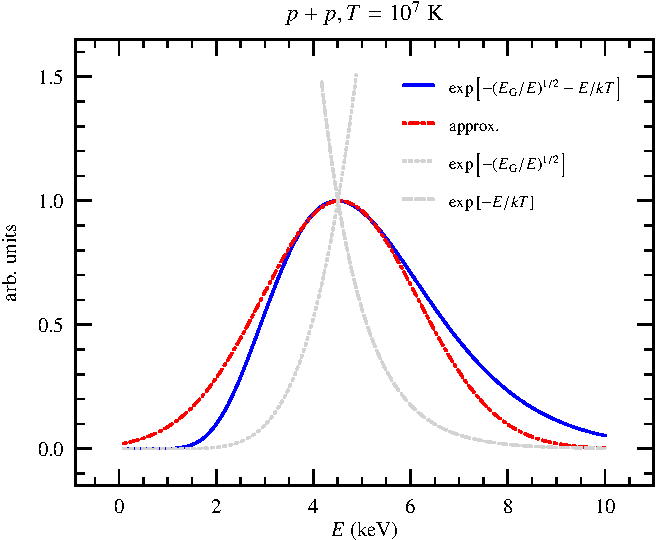
\includegraphics[width=4in]{coulomb_integrand}
\caption[Competition between Boltzmann factor and penetration of Coulomb barrier in setting the thermally-averaged reaction rate.]{Integrand of eq.~(\protect\ref{e.integral}) (\emph{solid line}) and the Gaussian (\emph{dot-dashed line}) constructed by expanding to second order the argument of the exponential. The parameters for $\EG$ were taken from the $p+p$ reactions ($Z_{1}Z_{2}=1$, $A = 1/2$), and the temperature is $10^{7}\nsp\K$.  Note that the grey curves, showing the two terms of the exponential, have been rescaled to fit on the same plot.}
\label{f.integrand}
\end{figure}

Another simplification can be made because both the Gaussian and the original integrand go to zero as $E\to 0$.  As a result, we can extend the lower bound of our integral (eq.~[\ref{e.integral2}]) to $-\infty$, and obtain
\begin{eqnarray}\label{e.rate2}
\langle\sigma v\rangle &\approx& \left(\frac{8}{\pi m}\right)^{1/2}\left(\frac{1}{kT}\right)^{3/2} S(\Epk) \exp\left[-3\left(\frac{\EG}{4kT}\right)^{1/3}\right]\frac{\Delta}{2}\nonumber\\
 &=& \frac{2^{13/6}}{\sqrt{3m}}\frac{\EG^{1/6}}{(kT)^{2/3}} \exp\left[-3\left(\frac{\EG}{4kT}\right)^{1/3}\right]  S(\Epk).
\end{eqnarray}
On to some numbers. Table~\ref{t.reaction} lists quantities for some common reactions. A couple of notes. First, $\Delta/\Epk$ indicates how well our Gaussian approximation works---you will see it is less than 1 in all cases. We evaluated $\Delta/\Epk$, which decreases with temperature as $T^{-1/6}$, at $T = 10^{7}\nsp\K$. Second, the quantity $n(T)$ is the exponent if we want to approximate the reaction rate as a power-law, $r\propto T^{n}$.  We compute this as 
\begin{equation}\label{e.exponent}
 n(T) = \frac{\dif\ln r}{\dif\ln T} = -\frac{2}{3} + \left(\frac{\EG}{4kT}\right)^{1/3},
 \end{equation}
 as you can easily verify for yourself. In the table, the exponent is evaluated at $T = 10^{7}\nsp\K$; obviously $n$ depends on temperature. Finally, note the size of $\EG/(4k)$.  This makes the argument of the exponential in equation~(\ref{e.rate2}) large in absolute value, and sets the temperature scale at which a given reaction comes into play.
 
\begin{table}[htbp]
\caption{\label{t.reaction} Parameters for non-resonant reactions}
\begin{center}
\begin{tabular}{lrrrrrr}
\hline
Reaction & $p+p$ & $p+\helium[3]$ & $\helium[3]+\helium[3]$ & $p+\lithium[7]$ & $p+\carbon$\\
\hline\hline
$A$ & 1/2 & 3/4 & 3/2 & 0.88 & 0.92 \\
$Z_{1}Z_{2}$ & 1 & 2 & 4 & 3 & 6 \\
$\EG$ (MeV) & 0.489 & $2.94$ & $23.5$ & $7.70$ & $32.5$\\
$\EG/(4k)$ (GK) & $1.4$ & $8.5$ & $68.0$ & $22.0$ & $94.0$ \\
$\Epk|_{T=10^{7}\nsp\K}$ (keV) & 4.5 & 8.2 & 16.3 & 11.3 & 18.2\\
$\Delta/\Epk|_{T=10^{7}\nsp\K}$ & 1.0 & 0.75 & 0.53 & 0.64 & 0.50 \\
$n(T = 10^{7}\nsp\K)$ & 4.6 & 8.8 & 18.3 & 12.4 & 20.5\\
\hline
\end{tabular}
\end{center}
\end{table}
%
%Once we have the reaction rate per pair of particles, the volumetric heating rate for the reaction $a+X$ is then
%\begin{equation}\label{e.heating-rate}
%\rho\varepsilon = Q\frac{n_{a}n_{X}}{1 + \delta_{aX}}\langle \sigma v\rangle.
%\end{equation}
%Now, $n_{a} = Y_{a}\rho/\mb$, where $Y_{a} = X_{a}/A_{a}$ is the abundance ($X_{a}$ is the mass fraction), and likewise for $n_{X}$. The denominator $1+\delta_{aX}$ takes care of double-counting if $a$ and $X$ are identical.

\section{Resonances}\label{s.resonant-reactions}

This section contains my condensed notes on resonances following Blatt and Weisskopf's excellent text\cite{Blatt1979Theoretical-Nuc}.  Other treatments of the subject, such as that in Iliadis\cite{Iliadis2007Nuclear-Physics} and in Clayton\cite{Clayton1983Principles-of-S}, mostly follow their approach. In this section, we shall often make use of the notation $X(a,b)Y$ to mean the reaction $X + a \to b + Y$.

\subsection{Orbitals}
Nuclei exhibit shell effects: one can often treat the nucleons as independent particles occupying orbitals determined by a mean force.  Unlike in the atomic case, the spin-orbit term in the Hamiltonian, $-a\bvec{L}\vdot\bvec{S}$, is quite strong. Since the total angular momentum is $\bvec{J}=\bvec{L}+\bvec{S}$, we have 
\[
\bvec{L}\vdot\bvec{S} = \frac{1}{2}\left(\bvec{J}\vdot\bvec{J} - \bvec{L}\vdot\bvec{L} - \bvec{S}\vdot\bvec{S}\right),
\]
and hence states with larger $\bvec{J}$ have a lower energy. The strong $\bvec{L}\vdot\bvec{S}$ coupling leads to the presence of ``gaps'' in the energy spectra; nuclei that have have filled (either neutrons or protons) shells up to this gap are unusually bound and the nucleon number (either neutron or proton) is termed a \emph{magic number}. The magic numbers are 2, 8, 20, 28, 50, 82, and 126. For example, \oxygen\ (8 protons, 8 neutrons) and \calcium\ (20 protons, 20 neutrons) are doubly magic and hence more strongly bound than other nuclides of similar mass.

We label the orbitals as $n\ell_{j}$, where $n$ is the radial quantum number, $\ell$ is the orbital angular momentum ($s,p,d,f,\ldots$), and $j$ is the total angular momentum.  The first few orbitals are listed in Table~\ref{t.orbitals}.  Each orbital has $2j+1$ nucleons, and a fully occupied orbital has $\bvec{J}=0$. For example, we would expect that the ground state of \carbon[13] (6 protons, 7 neutrons) to have closed $1s_{1/2}$ and $1p_{3/2}$ shells for both neutrons and protons, and the remaining neutron would then occupy the $1p_{1/2}$ shell.

\begin{table}[htbp]
\caption{\label{t.orbitals} Neutron orbitals}
\begin{center}
\begin{tabular}{ccc}
\hline
Orbital & Number, $2j+1$, in orbital & Total number\\
\hline\hline
$1d_{3/2}$ & 4 & 20\\
$2s_{1/2}$ & 2 & 16\\
$1d_{5/2}$ & 6 & 14\\
$1p_{1/2}$ & 2 & 8\\
$1p_{3/2}$ & 4 & 6\\
$1s_{1/2}$ & 2 & 2\\
\hline
\end{tabular}
\end{center}
\end{table}

The remaining quantum number is parity ($\bvec{\pi}$), which is conserved under the strong force. The parity of a nucleon orbital is $(-1)^{\ell}$, where the angular momentum number $\ell$ must be summed over all nucleons. Since a closed shell has an even number of nucleons, it must have positive parity. For example, the ground state of $\oxygen[17]$ has 8 protons filling the $1s_{1/2}$, $1p_{3/2}$, and $1p_{1/2}$ shells 8 neutrons in closed shells, so the remaining neutron must be in the  $1d_{5/2}$ shell ($\ell=2$): the angular momentum and parity of the ground state must therefore be $j^{\pi} = \frac{5}{2}^{+}$. As a second example, \nitrogen has 6 protons in closed shells and 6 neutrons in closed shells, with the remaining proton and neutron both in $1p_{1/2}$ orbitals.  Hence the angular momentum of the ground state could either be $0$ or $1$; it turns out that the symmetric state has lower energy, so $j=1$. The parity of the ground state is $(-1)^{1 + 1} = 1$, so $J^{\pi}( \nitrogen) = 1^{+}$.

The angular momentum matters because it sets the possible range of relative angular momenta that the incoming particles can have.  Writing the wave function as $\psi(r) = (u_{\ell}(r)/r)Y_{\ell 0}$ and substituting  into Schr\"odinger's equation,
\[
-\frac{\hbar^{2}}{2m}\nabla^{2}\psi + V(r)\psi  = E\psi,
\]
gives the following equation for $u_{\ell}$,
\[
\frac{\dif^{2}}{\dif r^{2}} u_{\ell} + \left\{ k^{2} - \frac{\ell(\ell + 1)}{r^{2}} - \frac{2m}{\hbar^{2}}\frac{Z_{a}Z_{X}e^{2}}{r} \right\}u_{\ell} = 0.
\]
Here $k$ is the wavenumber for the particle at $r\to\infty$, $E = \hbar^{2}k^{2}/2m$. Note the presence of the ``centrifugal barrier,''
\[ \frac{\hbar^{2}}{2mr^{2}} \ell(\ell+1)  = 20.9\nsp\MeV\frac{\mb}{m}\left(\frac{\fermi}{r}\right)^{2}\ell(\ell+1): \]
there is a price to pay if the particles must have a high relative $\ell$.

\subsection{Formation of a compound nucleus}
Even orbitals with positive energy can be long-lived; suppose we excite a proton in \carbon[11] to an orbital just above the threshold for decay into $\pt + \boron[10]$.  Although this state has positive energy and can decay, the particle has to tunnel through the coulomb barrier, and potentially an angular momentum barrier if $s$-wave emission is forbidden.  We saw that the probability of getting through the Coulomb barrier (for $s$-wave) is given by eq.~(\ref{e.prob}).  If this is very small, then we can imagine a classical particle oscillating back and forth in the well, which is does many times because the probability of escaping each time it approaches the barrier is so small. Thus, if there is a substantial energy barrier impeding escape, the classical oscillation period $P$ is much less than the lifetime of the state $\tau$.  Now the classical oscillation period depends inversely on the spacing $D$ between energy levels, $P \sim \hbar/D$, as you can verify for an infinite square well potential.  Hence if the probability of tunneling is sufficiently small,
\[
 \frac{P}{\tau} \sim \frac{\hbar}{D\tau} = \frac{\Gamma}{D} \ll 1,
\]
where the width of the state to particle emission is $\Gamma = \hbar/\tau$.  Hence for reactions at low excitation energies involving light nuclei with widely separated levels, we can look at captures into discrete levels in the compound nucleus. 

\subsection{Derivation of resonant cross-section}\label{s.resonant-cross-section}
We're now ready to do some heavy lifting and derive the cross-section for a resonant reaction.  The nuclear force is short-ranged, so we can define a ``channel radius'' $R$ exterior to which our potential is purely Coulomb. Our strategy is just like doing transmission resonances in quantum mechanics: we'll solve for the wave function exterior to $R$ and match it to the wave function inside $R$.  Since we don't completely know the form of the potential inside $R$, our expression will have terms that must be experimentally constrained.

The reaction is $a + X$; the coulomb potential is $Z_{a}Z_{X}e^{2}/r$ and the relative angular momentum of $a$ and $X$ is $\ell$.  Let $m$ be the reduced mass of $a$ and $X$.  Our wave function is then $\psi(r) = (u_{\ell}(r)/r)Y_{\ell 0}$; substituting this into the Schr\"odinger equation,
\[
-\frac{\hbar^{2}}{2m}\nabla^{2}\psi + V(r)\psi  = E\psi,
\]
gives the following equation for $u_{\ell}$,
\[
\frac{\dif^{2}}{\dif r^{2}} u_{\ell} + \left\{ k^{2} - \frac{\ell(\ell + 1)}{r^{2}} - \frac{2m}{\hbar^{2}}\frac{Z_{a}Z_{X}e^{2}}{r} \right\}u_{\ell} = 0.
\]
Here $k$ is the wavenumber for the particle at $r\to\infty$, $E = \hbar^{2}k^{2}/2m$. There are two solutions to this differential equation; the solutions are known as Coulomb wave functions, $F_{\ell}$ and $G_{\ell}$.  The regular solution $F_{\ell}$ vanishes as $r\to 0$, and $G_{\ell}$ blows up at the origin. 
For $kr \gg 1$, the Coulomb wave functions go over to
\begin{eqnarray}\label{e.coulombF}
F_{\ell}(r) &\simeq& \sin\left[ kr - \frac{1}{2}\ell\pi -\gamma\ln(2kr) + \sigma_{\ell}\right]\\
G_{\ell}(r) &\simeq& \cos\left[ kr - \frac{1}{2}\ell\pi -\gamma\ln(2kr) + \sigma_{\ell}\right].
\label{e.coulombG}
\end{eqnarray}
Here the parameter $\sigma_{\ell}$ is a Coulomb phase shift, and the parameter
\[ \gamma = \frac{1}{2\pi}\left(\frac{E_{G}}{E}\right)^{1/2} \]
contains the Gamow energy.  This shouldn't be too surprising: since $F_{\ell}$ and $G_{\ell}$ are the exact solutions to the motion of a particle in a Coulomb potential, they must behave like what we found using a WKB approximation in some limit.

For $r \geq R$, we can write our solution in terms of outgoing waves, $u_{\ell}^{+}$, and incoming waves, $u_{\ell}^{-}$; here the outgoing and incoming waves are defined as 
\begin{eqnarray*}
u_{\ell}^{+} &=& e^{-i\sigma_{\ell}}\left[G_{\ell} + i F_{\ell}\right]\\
u_{\ell}^{-} &=& e^{i\sigma_{\ell}}\left[G_{\ell} - i F_{\ell}\right].
\end{eqnarray*}
At large distances these go over to plane waves,  and so we can determine the coefficients,
\begin{equation}\label{e.coulomb-solution}
u_{\ell} = \frac{\sqrt{\pi}}{k}i^{2\ell + 1}(2\ell +1)^{1/2}\left[u_{\ell}^{-} - \eta_{\ell}u_{\ell}^{+}\right].
\end{equation}
The effect of the nucleus is to affect the outgoing waves via the coefficient $\eta_{\ell}$.  Furthermore, if we integrate the current over a large sphere we obtain the cross-section for the reaction (if the current is zero, then every particle that enters the sphere leaves it, so there is no reaction),
\begin{equation}\label{e.cross-section-eta}
\sigma_{\ell} = \frac{\pi}{k^{2}}(2\ell +1) \left[ 1 - |\eta_{\ell}|^{2}\right].
\end{equation}
To determine $\eta_{\ell}$, we need to find the logarithmic derivative
\[
\alpha_{\ell} \equiv R\left.\frac{u_{\ell}'}{u_{\ell}}\right|_{r=R}
\]
where $u_{\ell}' = \dif u_{\ell}/\dif r$.  For now $\alpha_{\ell}$ is undetermined, since it depends on the wave function inside the nucleus.  It is useful to define the following quantities:
\begin{eqnarray}\label{e.coulombPhase}
\frac{u_{\ell}^{-}}{u_{\ell}^{+}} & = & \frac{G_{\ell} - i F_{\ell}}{G_{\ell} + i F_{\ell}}e^{2i\sigma_{\ell}} \equiv e^{2i\xi}\\
R\left.\frac{u_{\ell}^{+'}}{u_{\ell}^{+}}\right|_{r=R} &=& R(G_{\ell}'G_{\ell} + F_{\ell}'F_{\ell})v_{\ell} + i kR v_{\ell} \equiv \Delta_{\ell} + is_{\ell}.
\label{e.delta-s}
\end{eqnarray}
In the last equation, we made use of the fact that $G_{\ell}F_{\ell}' - F_{\ell}G_{\ell}' = k$ for all $r$ and defined
\[
v_{\ell} = \left(G_{\ell}^{2} + F_{\ell}^{2}\right)^{-1}_{r=R}.
\]
To see the significance of $v_{\ell}$, note that the ratio of an outgoing wave at $r\to\infty$ and that at $r=R$ is
\[
\frac{|u_{\ell}(\infty)|^{2}}{|u_{\ell}(R)|^{2}} = \frac{1}{G_{\ell}^{2}(R) + F_{\ell}^{2}(R)},
\]
where the numerator follows from the asymptotic forms, eqns.~(\ref{e.coulombF}) and (\ref{e.coulombG}). This ratio, however, is just the probability of the wave transmitting through the potential barrier, and for $\ell=0$ is approximately what we found earlier (eq.~[\ref{e.prob}]) using the WKB approximation.

Evaluating $\alpha_{\ell}$ for the solution defined at $r \geq R$, eq.~(\ref{e.coulomb-solution}), and using our definitions, eq.~(\ref{e.coulombPhase}) and (\ref{e.delta-s}), we determine the phase shift,
\[
\eta_{\ell} = \frac{\alpha_{\ell} - \Delta_{\ell} + is_{\ell} }{\alpha_{\ell} - \Delta_{\ell} -i s_{\ell}}e^{2i\xi}.
\]
Using this to evaluate the reaction cross-section, eq.~(\ref{e.cross-section-eta}), we have
\begin{equation}\label{e.cross-section-alpha}
\sigma_{\ell} = \frac{\pi}{k^{2}}(2\ell +1) \frac{-4s_{\ell}\Im\alpha_{\ell}}{(\Re\alpha_{\ell}-\Delta_{\ell})^{2} + (\Im\alpha_{\ell} - s_{\ell})^{2}}
\end{equation}
Notice that the reaction cross-section vanishes if $\alpha_{\ell}\in\mathbb{R}$, i.e., $\Im\alpha_{\ell}=0$.  So far, our efforts may just look like we are reshuffling terms for no apparent reason, but there is a method to the algebraic madness. We see explicitly, for example, that the cross-section is proportional to the penetration through the term $s_{\ell}$ in the numerator.

To make further progress, we have to evaluate $\alpha_{\ell}$, and this requires making some constraints on the form of the wavefunction at $r < R$. Although the precise form of the potential is unknown, we do know that it is a rather deep well.  Just inside the surface $R$, we expect the radial wavefunction to be composed of spherical waves,
\[
u_{\ell}(r<R) = A\left\{\exp(-iKr) + e^{2i\zeta}e^{-2q}\exp(iKr)\right\}.
\]
Our reasoning for this form is as follows.  In general the state will be a standing wave, which we can write as a sum of incoming and outgoing waves.  The jump in the potential at $r=R$ introduces a phase shift, which we parameterize by $e^{2i\zeta}$. If the state decays by another channel than simply re-emitting the particle, i.e. if a reaction occurrs, then the amplitude of the outgoing wave will be less than that of the incoming wave; we parameterize this by the factor $e^{-2q}$.  We expect that $q\ll 1$, because otherwise the state wouldn't be long-lasting and have a well-defined energy.

We can factor $u_{\ell}(r<R)$,
\begin{eqnarray*}
u_{\ell}(R) &=& \left(2A e^{i\zeta}e^{-q}\right)\left\{\frac{\exp(-iKR -i \zeta + q) + \exp(iKR + i \zeta - q)}{2}\right\} \\
 &=& C\cos(KR+\zeta + iq).
\end{eqnarray*}
Using this to evaluate the logarithmic derivative,
\begin{equation}\label{e.alpha}
\alpha_{\ell} = -KR\tan(KR + \zeta + iq).
\end{equation}
Now, recall that $K \gg k$; the wavenumber inside the nuclear potential well is much larger than that outside.  The only way to smoothly join two waves with such discrepant wavenumbers is to have them match where $u_{\ell}' = 0$, i.e., where $\alpha_{\ell} = 0$.  Let's expand $\alpha_{\ell}$ about such a point with energy $\varepsilon_{r}$ and $q = 0$:
\[
\alpha_{\ell} \approx \left.\frac{\partial\alpha_{\ell}}{\partial \varepsilon}\right|_{q=0,\varepsilon=\varepsilon_{r}}(\varepsilon - \varepsilon_{r}) + \left.\frac{\partial\alpha_{\ell}}{\partial q}\right|_{q=0,\varepsilon=\varepsilon_{r}} q.
\]
Substituting this into equation~(\ref{e.cross-section-alpha}) gives
\begin{equation}\label{e.sigma-penultimate}
\sigma = \frac{\pi}{k^{2}}(2\ell+1)\left\{\frac{ 4KRq s_{\ell}}{[(\partial_{\varepsilon}\alpha_{\ell})(\varepsilon - \varepsilon_{r}) - \Delta_{\ell}]^{2} + [ -KRq - s_{\ell}]^{2}}\right\}.
\end{equation}
We expect that near a resonance, the cross-section will have a Lorentzian profile, with a total width
\[
\Gamma = \sum_{i}\Gamma_{i} + \Gamma_{\gamma}
\]
that is the sum of particle decay widths $\Gamma_{i}$ and widths for radiative transitions $\Gamma_{\gamma}$.  The entrance channel width will be proportional to $s_{\ell}=kRv_{\ell}$. Furthermore, a reaction will take place if the nucleus does something other than decay in the entrance channel, and this will occur with probability $\Gamma - \Gamma_{a}$.  

Motivated by these considerations, we note that
if we define the width for decay in the entrance channel as
\begin{equation}\label{e.Gamma-entrance}
\Gamma_{a} = -\frac{2s_{\ell}}{\partial_{\varepsilon}\alpha_{\ell}} = -\frac{2kR\,v_{\ell}}{\partial_{\varepsilon}\alpha_{\ell}},
\end{equation}
the reaction width as (it can be shown that in general $\partial_{\varepsilon}\alpha_{\ell} < 0$)
\begin{equation}\label{e.Gamma-reaction}
\Gamma_{r} = \Gamma-\Gamma_{\alpha} = -\frac{2KR\,q}{\partial_{\varepsilon}\alpha_{\ell}},
\end{equation}
and the ``observed'' resonance energy as 
\[
\varepsilon_{r,\mathrm{obs}} = \varepsilon_{r} + \frac{\Delta_{\ell}}{\partial_{\varepsilon}\alpha_{\ell}},
\]
then the cross-section becomes
\begin{equation}\label{e.breit-wigner}
\sigma = \frac{\pi}{k^{2}}(2\ell + 1)\frac{\Gamma_{a}\Gamma_{r}}{(\varepsilon - \varepsilon_{r,\mathrm{obs}})^{2} + (\Gamma/2)^{2}}.
\end{equation}
This is the cross-section for a compound nucleus to form in channel $a$ and decay by any other channel.  To get the cross-section for a specific exit channel $b$, we must multiply by the branching ratio $\Gamma_{b}/\Gamma_{r}$.  Finally, for an unpolarized incident beam, we need to multiply the cross section by a statistical factor
\begin{equation}\label{e.stat-factor}
\omega = \frac{2J + 1}{(2J_{a}+1)(2J_{X}+1)}
\end{equation}
to account for the fraction of angular momentum states in the target $X$ and beam $a$ that can enter the level with the appropriate angular momentum $\ell$.

You might be troubled by our identification of the particle width, eq.~(\ref{e.Gamma-entrance}), and reaction width, eq.~(\ref{e.Gamma-reaction}). Notice that if we were to solve the problem of a quasi-bound state leaking out of its well, we would encounter similar equations, and this would lead to the identification of the level width.  We can make the argument more plausible by the following consideration.  Let's consider $\partial_{\varepsilon}\alpha_{\ell}$, evaluated about the point where $\alpha_{\ell} = 0$ and $q= 0$.  The general form of $\alpha_{\ell}$ is a tangent function (eq.~[\ref{e.alpha}]), so if we increase the energy by the spacing between levels $D$, the phase of the tangent must increase by $\pi$.  Hence, $\partial_{\varepsilon}\alpha_{\ell}|_{KR + \zeta = n\pi, q=0} \sim -KR\pi/D$. Substituting this into eq.~(\ref{e.Gamma-entrance}) and rearranging,
\[
\Gamma_{a} \sim \hbar \left(\frac{4k}{K}\right)\left(\frac{D}{2\pi\hbar}\right)v_{\ell}.
\]
Now, when a plane wave is incident on a step in the potential, the transmission coefficient across the step is roughly $k/K$, as you can verify by solving a one-dimensional Schr\"odinger equation.  We saw earlier that classical oscillation period for a particle in a well is $2\pi\hbar/D$. Hence 
\begin{eqnarray*}
\lefteqn{\Gamma_{a} \sim \hbar\times(\textrm{oscillation frequency})}\\
&& \times(\textrm{transmission across potential step at nuclear surface})\\
 && \times(\textrm{probability of penetrating coulomb, centrifugal barrier}).
\end{eqnarray*}
But this is precisely what we would write down for $\hbar\times(\textrm{rate of decay in channel $a$})$---the particle has a small probability on each oscillation to penetrate the potential jump and barrier.

\subsection{A worked example}

Consider the reaction $\boron[10](\pt,\alpha)\beryllium[7]$. We can think of this reaction proceeding first via the formation of a compound nucleus in an excited state, $\carbon[11]^{\star}$. It can be shown that the cross-section for the formation of $\carbon[11]^{\star}$ via proton capture is proportional to the width for the decay of that state via proton emission: 
\begin{equation}\label{e.reciprocity}
\sigma(\pt + \boron[10]\to \carbon[11]^{\star}) \propto \Gamma_{\pt}.
\end{equation}
The second stage of the reaction is the decay of the $\carbon[11]^{\star}$ into $\alpha + \beryllium[7]$.
Because of the short timescale $\sim 10^{-23}\nsp\second$ for nuclear interactions---roughly the crossing time for a nucleon in a $20\nsp\MeV$ by $2\nsp\fermi$ well---we make the assumption that the decay of an excited state does not depend on how the state was formed. If $\Gamma_{\alpha}$ represents the decay $\carbon[11]^{\star}\to \alpha+\beryllium[7]$, then
\[ \sigma(\pt + \boron[10] \to \alpha+\beryllium[7]) \propto \Gamma_{\pt}\Gamma_{\alpha}. \]
The full expression for the cross section is
\begin{equation}\label{e.resonant-cross-section}
 \sigma(\pt + \boron[10] \to \alpha+\beryllium[7])  = \frac{\pi}{k^{2}}(2\ell + 1)\omega\frac{\Gamma_{\pt}\Gamma_{\alpha}}{(\varepsilon - \varepsilon_{r,\mathrm{obs}})^{2} + (\Gamma/2)^{2}}.
\end{equation}
Here the first term $\pi(2\ell+1)k^{-2}$ is the geometrical cross-section and $\Gamma$ represents the total decay width of the excited state in the compound nucleus.  The factor $\omega$  is the statistical factor
\[
\omega = \frac{2J + 1}{(2J_{\pt}+1)(2J_{10}+1)}
\]
that accounts for the fraction of angular momentum states that can enter the level with the appropriate angular momentum $\ell$.
For our example, the reaction $\boron[10](\pt,\alpha)\beryllium[7]$ can proceed via  the $J^{\pi} = 5/2^{+}$ level at $8.70\nsp\MeV$ in \carbon[11].  The angular momentum and parity of \boron[10] and the proton are $J^{\pi}(\boron[10]) = 3^{+}$, $J^{\pi}(\pt) = 1/2^{+}$.  These two spins can add to either $7/2^{+}$ (multiplicity of 8) or $5/2^{+}$ (multiplicity of 6).  As a result, they can enter into the resonance with $\ell = 0$, and they will do so with $6/14$ probability.  The cross section for this reaction is then
\[
\sigma(\pt + \boron[10]\to\beryllium[7]+\alpha) = \frac{6}{14}\frac{\pi}{k^{2}}\frac{\Gamma_{\pt}\Gamma_{\alpha}}{(\varepsilon-\varepsilon_{8.70})^{2} + (\Gamma/2)^{2}}.
\]
This is multiplied by the entrance channel velocity $v$ and integrated over the thermal distribution to produce the reaction rate.

\section{Inverse Rates}\label{s.inverse-rates}

Consider a photodisintegration reaction $Y(\gamma,a)X$.  We could compute the rate for this by first computing the excitation $Y\to Y^{*}$ by absorption of a photon followed by decay through the $a$-channel.  There is another, easier, way to compute the thermally averaged rate, however, if we already have an expression for the forward reaction $X(a,\gamma)Y$.  Suppose we allow our plasma, consisting of $a$, $X$, and $Y$ to come into thermal balance.  In such a plasma, the composition does not change with time, so our forward and inverse rates must balance:
\begin{equation}\label{e.balanced-rates}
 n_{X}n_{a}\langle \sigma v \rangle_{Xa} = n_{Y}\lambda,
\end{equation}
where $\lambda$ is the photodissociation rate.  Since we are in thermal equilibrium, however, we also have a relation between the chemical potentials,
\[ \mu_{X} + \mu_{a} = \mu_{Y}. \]
For an ideal gas, the chemical potentials are given by eq.~(\ref{e.chem-pot-ideal-gas}). Rearranging terms gives and taking the exponential gives us the equation
\begin{equation}\label{e.Xa-Y}
	\frac{n_{X}n_{a}}{n_{Y}} = \frac{n^{Q}_{X}n^{Q}_{a}}{n^{Q}_{Y}}\exp\left(-\frac{Q}{\kB T}\right).
\end{equation}
In this expression we have substituted $Q = (m_{a}+m_{X}-m_{Y})c^{2}$, and 
\[
	n^{Q}_{i} = g_{i}\left(\frac{m_{i}\kB T}{2\pi\hbar^{2}}\right)^{3/2}.
\]
Substituting eq.~(\ref{e.Xa-Y} into eq.~(\ref{e.balanced-rates}) gives us an expression for the photodissociation rate $\lambda$ in terms of the forward rate,
\begin{eqnarray}
 \lambda &=& \frac{n_{X}n_{a}}{n_{Y}} \langle \sigma v \rangle_{Xa} \nonumber\\
 \label{e.inverse-from-balance}
 &=& \frac{g_{X}g_{a}}{g_{Y}} \left(\frac{\mb \kB T}{2\pi\hbar^{2}}\right)^{3/2} \left(\frac{A_{X}A_{a}}{A_{Y}}\right)^{3/2} \exp\left(-\frac{Q}{\kB T}\right) \langle \sigma v \rangle_{Xa}.
\end{eqnarray}
This expression is specific to this type of reaction, but similar formula can be generated for other types of reactions, such as $X(a,b)Y$.

\section{Plasma corrections to the reaction rate}\label{s.correction-penetration}

In stars, the nuclear reactions do not occur in isolation, but rather in the midst of a plasma.  The effect of these ambient charges is to screen the long-range Coulomb interaction. This in turn perturbs the penetration factors and hence the reaction rates. We now derive the lowest order correction \cite{Salpeter1954Electrons-Scree}. 

The first thing to consider are the typical scales involved.  In a plasma, the mean interparticle spacing is 
\[ a = \left(\frac{3A\mb}{4\pi \rho}\right)^{1/3} = 1.6\ee{4}\nsp\fermi\times A^{1/3}\left(\frac{100\nsp\grampercc}{\rho}\right)^{1/3},
\]
and the Debye length (cf.\ eq.~[\ref{e.linearized-Poisson}]) is 
\[
\lambdaD = 2.8\ee{4}\nsp\fermi\times \left(\frac{T}{10^{7}\nsp\K}\right)^{1/2} \left(\frac{100\nsp\grampercc}{\rho}\right)^{1/2} \left(\frac{A}{\langle Z^{2}+Z\rangle}\right)^{1/2}.
\]
Both of these lengths, for typical conditions in a stellar plasma, are much larger than the size of the classically forbidden region through which the particle must tunnel: at $\Epk = 10\nsp\keV$, this length is $\re = 144\,Z_{1}Z_{2}\nsp\fermi \ll a < \lambdaD$.  The nuclear scale is $\sim\fermi$ and is much smaller that all of these.

The penetration factor (eq.~[\ref{e.wkb}]) depends on the potential in the barrier; given that $\re \ll \lambdaD$, we may expand the potential, eq.~(\ref{e.screened-potential}), and write
\begin{equation}
\mathcal{P} \propto \exp\left\{\frac{2}{\hbar}\int_{\re}^{\rn}\left[2m\left(\frac{Z_{1}Z_{2}e^{2}}{r} - \frac{Z_{1}Z_{2}e^{2}}{\lambdaD} - E\right) \right]^{1/2}\,\dif r\right\}.
\end{equation}
Since $\lambdaD$ doesn't depend on either $E$ or $r$, the effect of the screening potential is just to  change the zero point of the energy scale.  Assuming the $S$-factor doesn't depend sensitively on energy, the effect of screening on the rate is just to multiply the integrand in equation~(\ref{e.rate}) by
\begin{equation}\label{e.fscreening}
  f_{\mathrm{scr}} = \exp\left(\frac{Z_{1}Z_{2}e^{2}}{\lambdaD\kB T}\right).
\end{equation}
Since this factor doesn't depend on $E$, it simply multiplies the rate $\langle\sigma v\rangle$.  Note that since $\lambdaD > a$ and since $e^{2}/(a\kB T) \ll 1$ in a plasma, this screening factor is a small correction to the rate.

\section{Equations for Chemical Evolution}\label{e.eqns-for-chem-evol}

Now that we have a reaction cross-section, we can write down the equations describing the chemical evolution of the star, and the nuclear heating. To make this concrete, let's look at the reaction $\pt + \pt \to e^{+}\nu_{e} + \hydrogen[2]$. The reaction rate is (cf.\ eqs.~[\ref{e.rate}] and [\ref{e.fscreening}])
\[ r_{pp} = \frac{1}{2} n_{\mathrm{H}}^{2}f^{\mathrm{scr}}_{pp}\langle\sigma v\rangle_{pp}. \]
Each reaction destroys 2 protons, so we can write down our equation for the change in $n_{\mathrm{H}}$,
\begin{equation}\label{e.H-conservation-1}
\partial_{t} n_{\mathrm{H}} + \divr(n_{\mathrm{H}}\vu) = -n_{\mathrm{H}}^{2} f^{\mathrm{scr}}_{pp} \langle\sigma v\rangle_{pp}.
\end{equation}
Likewise, the $pp$ reaction produces deuterium, which is in turn destroyed by $\mathrm{D} + \pt \to \helium[3]$:
\begin{equation}\label{e.H-conservation-2}
\partial_{t} n_{\mathrm{D}} + \divr(n_{\mathrm{D}}\vu) = \frac{1}{2} n_{\mathrm{H}}^{2} f^{\mathrm{scr}}_{pp}\langle\sigma v\rangle_{pp} - n_{\mathrm{D}} n_{\mathrm{H}} f^{\mathrm{scr}}_{Dp}\langle\sigma v\rangle_{Dp}.
\end{equation}
Let's write each number density in terms of its abundance: $n_{\mathrm{H}} = Y_{\mathrm{H}}\NA\rho$. We can then use the equation of mass continuity (eq.~[\ref{e.mass-1}]) to simplify these equations to
\begin{eqnarray}
\left(\partial_{t} + \vu\vdot\grad\right) Y_{\mathrm{H}}  &=& -Y_{\mathrm{H}}^{2}\rho f^{\mathrm{scr}}_{pp} \left[\NA\langle\sigma v\rangle\right]_{pp}\label{e.H-abund} \\
\left(\partial_{t}  + \vu\vdot\grad\right) Y_{\mathrm{D}} &=& \frac{1}{2} Y_{\mathrm{H}}^{2}\rho f^{\mathrm{scr}}_{pp} \left[\NA\langle\sigma v\rangle\right]_{pp} \nonumber\\ && {}- Y_{\mathrm{D}} Y_{\mathrm{H}} \rho f^{\mathrm{scr}}_{Dp}\left[\NA \langle\sigma v\rangle\right]_{Dp}. \label{e.D-abund}
\end{eqnarray}
The left-hand side of these equations are just the Lagrangian time derivatives. On the right-hand sides, the quantities in $[\,]$ are just functions of temperature and are compiled into rate libraries, such as \textsc{reaclib}.
We will need equations like (\ref{e.H-abund}) and (\ref{e.D-abund}) for each species in our star. A collection of such equations is known as a \textbf{reaction network}.

Each reaction is specified by a $Q$-value, which is just the energy deposited into the gas by the reactions. If there is no neutrino released, this will just be the change in nuclear binding energy, but for reaction like $\pt + \pt$ one has to account for the energy carried off by the neutrino.  For the two reactions we consider here, the total heating rate, per unit mass, is
\begin{eqnarray}
q &=& \frac{1}{\rho}\left(\frac{Q_{pp}}{2}n_{\mathrm{H}}^{2} f^{\mathrm{scr}}_{pp}\langle\sigma v\rangle_{pp} + Q_{DP} n_{\mathrm{D}}n_{\mathrm{H}} f^{\mathrm{scr}}_{Dp}\langle\sigma v\rangle_{Dp}\right)\\
 &=& \frac{Q_{pp}\NA}{2}Y_{\mathrm{H}}^{2}\rho f^{\mathrm{scr}}_{pp} \left[\NA\langle\sigma v\rangle\right]_{pp} \nonumber \\
 && {}+ Q_{Dp}\NA Y_{\mathrm{D}}Y_{\mathrm{H}} \rho f^{\mathrm{scr}}_{Dp} \left[\NA\langle\sigma v\rangle\right]_{Dp} .
\label{e.heating-rate}
\end{eqnarray}
The equations for the change in chemical composition and the heating rate close our system of equations describing the structure and evolution of the star.  We are now ready to discuss the life cycle of stars in detail.
 
% !TEX root = ./stellar-notes.tex
\chapter[Main Sequence]{Hydrogen Burning and the Main Sequence}

\section[The pp chain]{Hydrogen burning via pp reactions: the lower main sequence}
\label{s.lower-ms}

In a contracting pre-main sequence star, the reaction $\hydrogen[2](p,\gamma)\helium[3]$ proceeds rapidly owing to the small Coulomb barrier; in fact, this reaction can occur in objects as small as $\approx 12\,M_{\mathrm{Jupiter}}$.  The small primordial abundance of deuterium, however, prevents this reaction from doing anything more than slowing contraction slightly.  The reaction $\pt +\pt$ is much slower, because there is no bound nucleus \helium[2]; the only possible way to form a nucleus is to have a weak interaction as well, giving the reaction $\pt(\pt,e^{+}\nu_{e})\hydrogen[2]$.

The weak cross section goes roughly as $\sigma_{\mathrm{weak}} \sim 10^{-20}\nsp\barn\left(E/\keV\right)$, so that
\[ \frac{\sigma_{\mathrm{weak}}}{\sigma_{\mathrm{nuc}}} \sim 10^{-23}\left(\frac{E}{\keV}\right). \]
The $S$-factor for the $\pt+\pt$ reaction is very small, and as a result the characteristic temperature for this reaction to occur is $\approx 1.5\ee{7}\nsp\K$; at this temperature, the lifetime of a proton to forming deuterium via capture of another proton is about $6\nsp\Giga\yr$.  Once a deuterium nucleus is formed, it is immediately destroyed via $\hydrogen[2](p,\gamma)\helium[3]$. The nucleus \lithium[4] is unbound with a lifetime of $10^{-22}\nsp\second$; the nucleus \beryllium[6] is likewise unbound ($\tau \sim 5\ee{-21}\nsp\second$). As a result, the next reaction that can occur is $\helium[3](\helium[3],2\pt)\helium$.  Despite having a much greater Gamow energy than $\pt + \pt$ (see Table~\ref{t.reaction}), this reaction still is much faster than $\pt+\pt$ owing to the small weak cross-section.

In addition to capturing another \helium[3], it is also possible that
\begin{eqnarray}
\helium[3] + \helium &\to& \beryllium[7] + \gamma\nonumber\\
 \beryllium[7] + e^{-} &\to& \lithium[7] +  \nu_{e}\qquad(\tau=53\nsp\unitstyle{d})\nonumber \\
 \lithium[7] + \pt &\to& 2\helium + \gamma;
 \end{eqnarray}
furthermore, at slightly higher temperatures \beryllium[7] can capture a proton instead of an electron, giving the third branch
\begin{eqnarray}
\beryllium[7] + \pt &\to& \boron[8] + \gamma\nonumber\\
\boron[8] &\to& \beryllium[8] + e^{+} + \nu_{e}\qquad(\tau = 770\nsp\milli\second)\nonumber\\
\beryllium[8] &\to& 2\helium\qquad(\tau=10^{-16}\nsp\second).
\end{eqnarray}
 The end result of these chains is the conversion of hydrogen to helium, although the amount of energy carried away by neutrinos differs from one chain to the next.


\begin{exercisebox}
 Compute the mass of H, in units of solar masses, that must be converted into \helium\ in order to supply the solar luminosity over $10^{10}\nsp\yr$.
\end{exercisebox}

\section[The CNO cycle]{Hydrogen burning via the CNO cycle: the upper main sequence}
\label{s.upper-ms}

As we saw in the previous section, the smallness of the $\pt+\pt$ cross-section means that captures onto heavier nuclei can be competitive at stellar temperatures.  Let's get a rough estimate of how charged a nucleus can be before the Coulomb barrier makes the reaction slower than $\pt+\pt$.  Assuming $A = 2Z$, and taking the $S$-factor for $\pt+\pt$ to be $10^{-22}$ times smaller that that for $\pt + \mathrm{^{A}Z}$ gives us the rough equation
\[ 10^{-22}\exp\left(-\frac{33.81}{T_{6}^{1/3}}\right) \approx \exp\left(-\frac{41.47 Z^{2/3}}{T_{6}^{1/3}}\right), \]
where the factors in the exponentials come from the peak energy for the reaction (see eq.~[\ref{e.exponent}]), and $T_{6}\equiv (T/10^{6}\nsp\K)$.  Solving for $Z$, we see that at $T_{6} = 10$, proton captures onto \carbon\ have a comparable cross-section to $\pt + \pt$; at $T_{6} = 20$, proton captures onto \oxygen\ have a comparable cross-section.

Thus at temperatures slightly greater than that in the solar center, the following catalytic cycle becomes possible.
\begin{center}
\begin{tabular}{rr}
reaction & $\log[(\tau/\yr) \times (\rho X_{H}/100\nsp\grampercc)]$\\
\hline
$\carbon(\underline{\pt},\gamma)\nitrogen[13]$ & 3.82\\
$\nitrogen[13](,e^{+}\nu_{e})\carbon[13]$ & $\tau=870\nsp\second$\\
$\carbon[13](\underline{\pt},\gamma)\nitrogen[14]$ & 3.21\\
$\nitrogen[14](\underline{\pt},\gamma)\oxygen[15]$ & 5.89 \\
$\oxygen[15](,e^{+}\nu_{e})\nitrogen[15]$ & $\tau = 178\nsp\second$\\
$\nitrogen[15](\underline{\pt},\underline{\helium})\carbon$ & 1.50 \\
\hline
\end{tabular}
\end{center}
As indicated by the underlined symbols, this cycle takes in 4 protons and releases 1 helium nucleus.
The reaction timescales are evaluated at a temperature of $20\nsp\Mega\K$.
The reaction $\nitrogen(\pt,\gamma)\oxygen[15]$ is by far the slowest step in the cycle; as a result, all of the CNO elements are quickly converted into \nitrogen\ in the stellar core, and this reaction controls the rate of heating.  At $T = 2\ee{7}\nsp\K$, $\dif \ln \varepsilon_{\mathrm{CNO}}/\dif\ln T = 18$; in contrast the $\pt+\pt$ reaction has a temperature exponent of only 4.5.

The strong temperature sensitivity of the CNO cycle has a profound effect on the properties of the upper main sequence.  Dividing equation~(\ref{e.lagrange-flux}) by equation~(\ref{e.lagrange-momentum}), we have
\begin{equation}\label{e.dTdP}
 \frac{\dif T}{\dif P} = \frac{3}{16\pi Gm}\frac{\kappa}{ac T^{3}}L_{r}.
\end{equation}
For stars with masses $\gtrsim \Msun$, the structure roughly follows a polytrope of index $n=3$.  We can insert the relations $T\sim M/R$ and $P\sim M^{2}/R^{4}$ into equation~(\ref{e.dTdP}) and scale to the solar luminosity to obtain 
\begin{equation}\label{e.L-M-upperMS}
L \approx L_{\odot} (M/\Msun)^{3}.
\end{equation}
On the other hand, we can integrate our equation for the heating rate per unit mass, $\varepsilon \approx \varepsilon_{0}\rho T^{n}$, over the star; inserting the scalings for $T$ and $\rho$ and normalizing to solar values, we obtain $L\approx L_{\odot} (M/\Msun)^{2+n}(R/\Rsun)^{-3-n}$. Equating this with $L$ from eq.~(\ref{e.L-M-upperMS}), we find that on the upper main sequence,
\begin{equation}\label{e.R-M-upperMS}
\frac{R}{\Rsun} \approx \left(\frac{M}{\Msun}\right)^{(n-1)/(n+3)}.
\end{equation}
For $n = 18$, this gives $R\sim M^{0.81}$.  Since $L = L_{\sun}(M/\Msun)^{3} = (R/\Rsun)^{2}(\Teff/T_{\mathrm{eff,\odot}})^{4}$, we can obtain a relation between $\Teff$ and $L$ on the upper main sequence,
\begin{equation}\label{e.Teff-L-upperMS}
\left(\frac{\Teff}{T_{\mathrm{eff,\odot}}}\right) = \left(\frac{L}{L_{\odot}}\right)^{0.12}.
\end{equation}
The fact that $\Teff$ is so insensitive to $L$ is a consequence that the radius increases with mass, which follows from the central temperature being roughly constant.  The strong temperature sensitivity of the CNO cycle ensures that the central temperature varies only slightly over a large range of luminosity.


\begin{exercisebox}
Suppose that there were no CNO cycle, and hydrogen could only be consumed via the PP chains.  Estimate the effective temperature-luminosity relation for the upper main-sequence in this case.  Would it be observationally distinguishable from the CNO-dominated upper MS?
\end{exercisebox}

A second effect on the stellar structure is that the luminosity is generated in a very small region concentrated about the center.  Inserting $P_{\mathrm{rad}} = (a/3) T^{4}$ and $\Ledd = 4\pi GMc/\kappa$ into equation~(\ref{e.dTdP}) and solving for $\nabla = \dif\ln T/\dif\ln P$, we obtain
\begin{equation}\label{e.del}
\nabla = \frac{1}{4}\frac{P}{P_{\mathrm{rad}}}\frac{L}{\Ledd}\left(\frac{L_{r}}{L}\right)\left(\frac{M}{M(r)}\right).
\end{equation}
For the Eddington standard model, $P/P_{\mathrm{rad}} \approx 2600 (M/\Msun)^{-2}$, and $L/\Ledd \approx 2.7\ee{-5} (M/\Msun)^{2}$.  Inserting these factors and using the criteria for convective stability, $\nabla < (\partial\ln T/\partial\ln P)_{S} = 2/5$,  we see that if 
\[ \frac{L_{r}}{L} > 23 \frac{M(r)}{M} \]
we have convective instability.  Thus, if the luminosity is produced in the innermost 4\% (by mass) of the star, the core will be convective.  The strong temperature sensitivity of the CNO reactions ensure that this is the case, and so the cores of upper main sequence stars have convective zones.

This convective zone changes the structure of the star, so that $L\sim M^{3.5}$ rather than the $M^{3}$ scaling used above.  It also means the star can burn more of the hydrogen in its interior.  The hotter $\Teff$ means, however, that the H$^{-}$ opacity is not important and the surface layers of upper main sequence stars are radiative.  Table~\ref{t.MS-characteristics} gives a summary of the properties of main sequence stars.

\begin{table}
\caption{\label{t.MS-characteristics} Characteristics of main-sequence stars}
\centering
\begin{tabular}{lll}
\hline
characteristic & lower ($M\lesssim\Msun$) & upper ($M\gtrsim\Msun$)\\
\hline\hline
hydrogen burning & pp & CNO\\
opacity & Kramers & Thomson\\
core & radiative, $\approx 0.1M$  & convective, $\approx 0.2 M$\\
envelope & convective & radiative\\
\hline
\end{tabular}
\end{table}

\newpage
\begin{exercisebox}
In this exercise, we are going to examine how the core of a solar-mass star approaches a steady conversion of 4 hydrogen nuclei to 1 helium nucleus via the PPI chain
\begin{eqnarray*}
 \pt + \pt &\to& e^{+} + \nu_{e} + \hydrogen[2]\\
 \hydrogen[2] + \pt &\to& \helium[3]\\
 \helium[3] + \helium[3] &\to& \helium + \pt + \pt.
 \end{eqnarray*}
Denote the abundances of protons, deuterium, \helium[3], and \helium\ by $Y_{p}$, $Y_{d}$, $Y_{3}$, and $Y_{4}$, respectively.  Furthermore, evaluate the rates at a fiducial central temperature and density (obtained with the \textsc{mesa} stellar evolution code) $T_{c,\odot} = 1.35\ee{7}\nsp\K$, $\rho_{c,\odot} = 83.2\nsp\grampercc$:
\begin{eqnarray*}
\lambda_{pp} \equiv \rho\NA\langle\sigma v\rangle(\pt+\pt \to \hydrogen[2]) &=& 4.40\ee{-18}\nsp\second^{-1} \\
\lambda_{pd} \equiv \rho\NA\langle\sigma v\rangle(\pt+\hydrogen[2] \to \helium[3])&=& 2.58\ee{-2}\nsp\second^{-1}\\
\lambda_{33} \equiv \rho\NA\langle\sigma v\rangle(\helium[3]+\helium[3]\to\helium[4]+\pt+\pt) &=& 3.40\ee{-9}\nsp\second^{-1}
\end{eqnarray*}
Take the screening factors to be unity.
\begin{enumerate}
\item First, let's consider the build-up of deuterium. Start from equation~(\ref{e.D-abund}):
\begin{equation}
\frac{\dif}{\dif t} Y_{d} = \frac{1}{2}Y_{p}^{2}\lambda_{pp} - Y_{d}Y_{p}\lambda_{pd}.
\end{equation}
Assume that over the timescale to establish the PP chain, the abundance of hydrogen $Y_{p}$ is constant, and that all the $\lambda$ are constant as well. Under these assumptions, solve for $Y_{d}(t)$ and show that it approaches a constant value
\[ \left.\frac{Y_{d}}{Y_{p}}\right|_{\mathrm{equil.}} = \frac{1}{2}\frac{\lambda_{pp}}{\lambda_{pd}}. \]
What is this abundance? What is the timescale to reach this equilibrium?

\item Now consider the evolution of \helium[3] via production by $d+\pt$ and destruction via $\helium[3]+\helium[3]$:
\begin{equation}
\frac{\dif}{\dif t}Y_{3} = Y_{p}Y_{d}\lambda_{pd} - Y_{3}^{2}\lambda_{33}.
\end{equation}
Again, under the assumption that $Y_{p}$ is constant, solve this equation for $Y_{3}(t)$. Use the value of the equilibrium value of $Y_{d}$, and show that $Y_{3}$ approaches a constant value
\[ \left.\frac{Y_{3}}{Y_{p}}\right|_{\mathrm{equil.}} = \left(\frac{1}{2}\frac{\lambda_{pp}}{\lambda_{33}}\right)^{1/2}. \]
What is this value? What is the timescale for the abundance of \helium[3] to reach 99\% of this equilibrium value? Is the assumption that deuterium is at its equilibrium abundance a valid one?
\item Using the equilibrium value of \helium[3], show that the rate of helium production via the $\helium[3]+\helium[3]$ is
\[ \frac{\dif}{\dif t}Y_{4} = \frac{1}{4}Y_{p}^{2}\lambda_{pp}. \]
\end{enumerate}
\end{exercisebox}

% !TEX root = ./stellar-notes.tex
\chapter[Low-Mass Post-Main Sequence]{Post-Main Sequence Evolution: Low-mass Stars}

\section{The Triple-Alpha Reaction}\label{s.triple-alpha}

The consumption of \helium\ is hindered by the lack of stable nuclei with mass numbers $A=5$ and $A=8$.  
The nucleus \beryllium[8] is, however, long-lived by nuclear standards: its decay width is $\Gamma = 68\nsp\eV$, implying a decay timescale $\hbar/\Gamma = 9.7\ee{-17}\nsp\second$.  (For comparison, the lifetime of \lithium[5] is $\sim 10^{-22}\nsp\second$.)  Thus if the reaction $\helium[4]+\helium[4]\to\beryllium[8]$ can proceed quickly enough, a small amount of $\beryllium[8]$ can accumulate allowing the reaction $\beryllium[8]+\helium\to\carbon$ to proceed.

The reaction $2\nsp\helium\to\beryllium[8]$ is endothermic, with $Q = -92\nsp\keV$.  As a result, the peak energy for Coulomb barrier transmission (see the discussion following eq.~[\ref{e.integral}]) must reach
\[ \Epk = \frac{\EG^{1/3}(kT)^{2/3}}{4^{1/3}} = -Q. \]
Substituting $\EG = 979\nsp\keV A (Z_{1}Z_{2})^{2}$ and solving for $T$ gives $T = 1.2\ee{8}\nsp\K$ as the temperature required to build up any substantial amount of \beryllium[8].  To reach such a temperature requires a helium core mass of $\gtrsim 0.45\nsp\Msun$.

Once a sufficient temperature is reached, the reaction $2\nsp\helium[4]\to\beryllium[8]$ comes into equilibrium with the decay, $\beryllium[8]\to2\nsp\helium$.  We can use a Saha-like equation (cf.\ eqns.~[\ref{e.ionization-chem-potential}] and [\ref{e.saha-eqn}]) to get the abundance of \beryllium[8].  Writing
\[ 2\mu_{4} = \mu_{8} - Q \]
and substituting the expression for $\mu$, eq.~(\ref{e.chem-pot-ideal-gas}) gives
\begin{equation}\label{e.n8-n4}
\frac{n_{8}}{n_{4}} = \left(\frac{2\pi\hbar^{2}}{\mb kT}\right)^{3/2}\left(\frac{8}{4^{2}}\right)^{3/2}\frac{X_{4}\rho}{4\mb}\exp\left(-\frac{92\nsp\keV}{kT}\right).
\end{equation}
Here we use $n_{8}$ and $n_{4}$ to mean the number densities of, respectively, \beryllium[8] and \helium; also $X_{4}$ denotes the mass fraction of helium.
Scaling eq.~(\ref{e.n8-n4}) to $\rho = \rho_{5} 10^{5}\nsp\grampercc$ and $T = T_{8}10^{8}\nsp\K$, we obtain
\begin{equation}\label{e.n8-to-n4}
 \frac{n_{8}}{n_{4}} = 2.8\ee{-5} T_{8}^{-3/2}X_{4}\rho_{5}\exp\left(-\frac{10.68}{T_{8}}\right).
\end{equation}
At $X_{4}\rho_{5}=1$ and $T_{8} = 1$, $n_{8}/n_{4} = 6.5\ee{-10}$.  

If the reaction $\beryllium[8]+\helium\to\carbon$ were non-resonant, the reaction rate for this $n_{8}$ would be far too slow to account for the amount of \carbon\ synthesized in stars.  Hoyle proposed, therefore, that there should be an excited state of the \carbon\ nucleus into which the reaction would proceed.  Both \helium\ and \beryllium[8] have spin and parity $J^{\pi} = 0^{+}$; hence for $s$-wave capture (angular momentum $\ell = 0$), the state in \carbon\ should also have $J^{\pi} = 0^{+}$.  What energy should the level have? The $Q$-value for $\beryllium[8]+\helium\to\carbon$ is $7.367\nsp\MeV$; the Gamow energy for this reaction is $\EG = 1.67\ee{5}\nsp\keV$ and hence the peak energy is $\Epk = 146\nsp\keV$, with a width $\Delta = 4(\Epk kT/3)^{1/2} = 82\nsp\keV$.  The proposed level should therefore have an energy within $2\Delta$ of $7.513\nsp\MeV$.

Such a level was indeed detected by Fowler, with $J^{\pi} = 0^{+}$ and $E = 7.654\nsp\MeV$.  Radiative decay from this level is hampered: the ground state also has $J^{\pi} = 0^{+}$, so the decay is forbidden; and the decay to the $J^{\pi}=2^{+}$ state at $4.44\nsp\MeV$ has a decay width of only $\Gamma_{\mathrm{rad}} = 3.67\milli\eV$.  This level's primary decay is indeed back to $\beryllium[8] + \helium$.  If the forward rate is fast enough, however, than a population of \carbon\ in this excited state can accumulate.  The total rate to the ground state would then be $n_{12*}\Gamma_{\mathrm{rad}}/\hbar$, where $n_{12*}$ is the number density of \carbon\ nuclei in the excited state.

To compute $n_{12*}$, we again can use the equation for chemical equilibrium: $\mu_{8} + \mu_{4} = \mu_{12*} - Q_{*}$.  Here $Q_{*} = -287\nsp\keV$ is the difference in energy between the \helium\ and \beryllium[8] nuclei and the energy of \carbon\ \emph{in the excited state.}  Again using eq.~(\ref{e.chem-pot-ideal-gas}) to expand $\mu$, we obtain
\begin{equation}\label{e.n12}
n_{12*} = \frac{n_{Q,12*}}{n_{Q,4}n_{Q,8}} n_{4}n_{8}\exp\left(-\frac{287\nsp\keV}{kT}\right).
\end{equation}
Substituting for $n_{8}$ using equation~(\ref{e.n8-n4}), this becomes
\begin{equation}\label{e.n12-2}
n_{12*} = \left(\frac{2\pi\hbar^{2}}{\mb kT}\right)^{3}\left(\frac{12}{4^{3}}\right)^{3/2} 
	\left(\frac{X_{4}\rho}{4\mb}\right)^{3} \exp\left(-\frac{397\nsp\keV}{kT}\right).
\end{equation}
Multiplying eq.~(\ref{e.n12-2}) by $\Gamma_{\mathrm{rad}}/\hbar$ and scaling to $\rho_{5}$, $T_{8}$, we obtain the net rate, per unit volume, at which $3\nsp\helium\to\carbon$,
\begin{equation}\label{e.triple-alpha}
 \textrm{rate} = 4.37\ee{31}\nsp\cm^{-3}\usp\second^{-1}\frac{(X_{4}\rho_{5})^{3}}{T_{8}^{3}}\exp\left(-\frac{44.0}{T_{8}}\right).
\end{equation}
Multiplying the rate by $Q = 7.275\nsp\MeV$, the net $Q$-value, gives the volumetric heating rate $\rho\varepsilon_{3\alpha}$, or
\begin{equation}\label{e.triple-alpha-heating}
\varepsilon_{3\alpha} \approx 5.1\ee{21}\nsp\ergs\usp\gram^{-1}\usp\second^{-1}\frac{X_{4}^{3}\rho_{5}^{2}}{T_{8}
^{3}}\exp\left(-\frac{44.0}{T_{8}}\right).
\end{equation}
The temperature exponent is $\dif\ln\varepsilon_{3\alpha}/\dif\ln T = 44.0/T_{8}-3$, that is, $\varepsilon_{3\alpha}\sim T^{41}$ at $T = 10^{8}\nsp\K$.

\subsection[Core helium burning]{The helium flash and the horizontal branch}\label{s.burning-stability}

The extreme temperature sensitivity of the triple-alpha reaction motivates a return to analyzing the stability of reactions in a stellar environment. We saw in an earlier problem that the ``gravithermal'' specific heat 
\[ C_{\star} \equiv T\left.\frac{\partial S}{\partial T}\right|_{M} < 0 \]
for an ideal gas. The physical cause is that an increase in entropy leads to an increase in radius, and the resulting $P\,\dif V$ work results in a reduced central temperature.

For conditions in low-mass stars at the time of helium ignition (nearly pure He at $T \approx 10^{8}\nsp\K$, $\rho \approx 10^{5}\nsp\grampercc$); at that density the temperature at $\kB T = \eF$ is (eq.~[\ref{e.TF}]) $4.1\ee{8}\nsp\K$.  Thus, He ignition takes place under semi-degenerate conditions.  To understand how the star responds, let's assume a homologous expansion---that is, one in which the ratios $r(m)/R(M)$ remains constant.  In other words, we assume that the structure of the star retains its functional form and we are merely ``rescaling'' our radial length.  To compute a gravithermal specific heat, we use Jacobians (see Appendix~\ref{s.thermo-derivatives}) to transform $S(T,P)$ to $S(T,M)$:
\begin{eqnarray}\label{e.homologous-cstar}
T\tderiv{S}{T}{M} &=& T\jac{S}{M}{T}{M}\nonumber \\
 &=& T\jac{S}{M}{T}{P}\jac{T}{P}{T}{M}\nonumber \\
 &=& T\tderiv{S}{T}{P} - T\tderiv{S}{P}{T}\tderiv{M}{T}{P}\tderiv{P}{M}{T}\nonumber \\
 &=& C_{P}\left[ 1 - \tderiv{T}{P}{S}\tderiv{P}{T}{M}\right],
\end{eqnarray}
where in the last identity we have used 
\[
 	\left(\frac{\partial T}{\partial P}\right)_{S} 
 	\left(\frac{\partial S}{\partial T}\right)_{P} 
 	\left(\frac{\partial P}{\partial S}\right)_{T} = -1
\]
and a similar expression relating $P$, $T$, and $M$. We could continue to use this technique of Jacobians to further transform $(\partial P/\partial T)_{M}$; but an easier method is to expand the equation of state as
\begin{equation}\label{e.eos-logarithmic}
\ln P = \chi_{\rho}\ln\rho + \chi_{T}\ln T,
\end{equation}
where $\chi_{\rho} \equiv (\partial\ln P/\partial\ln \rho)_{T}$, and similarly for $\chi_{T}$.  In an homologous expansion or contraction, the polytropic index stays constant, so that from equations~(\ref{e.LE-density-ratio}) and (\ref{e.LE-PC}) we have
\begin{equation}\label{e.homologous-eos-changes}
\tderiv{\ln P}{\ln R}{M} = -4,\qquad \tderiv{\ln\rho}{\ln R}{M} = -3.
\end{equation}
Using these relations, we have
\begin{eqnarray*}
 \tderiv{\ln T}{\ln R}{M} &=& \chi_{T}^{-1}\left[\tderiv{\ln P}{\ln R}{M} - \chi_{\rho}\tderiv{\ln\rho}{\ln R}{M}\right]\\
   &=& \frac{-4 + 3\chi_{\rho}}{\chi_{T}}.
\end{eqnarray*}
We can use this along with equations~(\ref{e.eos-logarithmic}) and (\ref{e.homologous-eos-changes}) to obtain
\begin{eqnarray}\label{e.dPdT-M}
 \tderiv{\ln P}{\ln T}{M} &=& \tderiv{\ln P}{\ln R}{M}\tderiv{\ln T}{\ln R}{M}^{-1}\nonumber \\
 &=& \frac{4\chi_{T}}{4-3\chi_{\rho}}.
\end{eqnarray}
Inserting eq.~(\ref{e.dPdT-M}) into equation~(\ref{e.homologous-cstar}), we finally get the expression for the gravithermal specific heat under a homologous expansion or contraction,
\begin{equation}\label{e.gravithermal-specific-heat}
	C_{\star} = C_{P}\left[1 - \nablaad\frac{4\chi_{T}}{4 - 3\chi_{\rho}}\right].
\end{equation}
For an ideal gas, $\chi_{T}=\chi_{\rho}=1$ and $\nablaad = 2/5$, so that $C_{\star} < 0$, as required for stability.  As the core becomes degenerate, however, $\chi_{\rho} \to 5/3$ and $\chi_{T}\to 0$; as a result, the addition of heat to the core causes the temperature to rise, causing the rate of heating from nuclear reactions to increase even further.  The ignition of helium in low-mass stars is therefore somewhat unstable and proceeds via ``flashes.''

Eventually, the burning of helium heats the core enough that degeneracy is lifted, and the star settles onto its ``helium main-sequence.''  On an HR diagram, low-mass stars with core helium burning lie on the ``horizontal branch.''

\subsection{The Asymptotic Giant Branch}\label{s.agb}

After exhaustion of helium burning in the core, the star has a semi-degenerate C/O core, surrounded by a He burning shell with a superincumbent H-burning shell.  Burning by these shells adds to the mass of the C/O core. As on the giant branch, the luminosity increases due to the high pressure at the edge of the core, and this high-luminosity produces a deep convective envelope, so that the star again lies along the Hayashi line in the HR diagram. 

Because of the large gravitational acceleration at the edge of the core, the burning shells become thin in radial extent.  This tends to make the burning unstable and leads to \emph{thermal pulses}.
To understand why the burning is unstable, let's revisit equation~(\ref{e.gravithermal-specific-heat}).  This equation still holds for expansion or contraction of a thin layer, with one critical difference: the volume of the shell is $4\pi r_{c}^{2}D$, where $D$ is the thickness of the shell and $r_{c}$ is the core radius, which is fixed. Hence if we expand or contract the shell, keeping the mass in the shell fixed, the logarithmic change in density is
\[ \dif\ln\rho = -\frac{\dif D}{D} = -\frac{\dif R}{D} = -\frac{R}{D}\dif\ln R. \]
Replacing the coefficient 3 of $\chi_{\rho}$ with $R/D$ in equation~(\ref{e.gravithermal-specific-heat}) gives us the specific heat during a homologous expansion or contraction of a shell of thickness $D$,
\begin{equation}\label{e.thin-shell-specific-heat}
 C_{\star,\mathrm{shell}} = C_{P}\left[1-\nablaad\frac{4\chi_{T}}{4-(R/D)\chi_{\rho}}\right].
\end{equation}
Even for an ideal gas, if $D < R/4$, say, then $C_{\star,\mathrm{shell}} > 0$ and the burning in the shell is thermally unstable.

When the burning shells are thin, the temperature, and hence rate of burning, become dependent on the local gravitational acceleration.  Because the underlying core is degenerate, this means the luminosity depends almost entirely on the core mass: an empirical fit is\cite{Paczynski1970Evolution-of-Si}
\begin{equation}\label{e.paczynski}
\frac{L}{\Lsun} = 5.9\ee{4}\left(\frac{M_{c}}{\Msun}-0.52\right).
\end{equation}
The rate at which mass is added to the core is set by the rate at which \hydrogen\ is processed into \helium,
\begin{equation}\label{e.mdot-core}
\frac{\dif M_{c}}{\dif t} = \frac{L}{q}.
\end{equation}
Here $q$ is the mass-specific energy release from the fusion of 4 \hydrogen\ into \helium: $q = 26.72\nsp\MeV/(4\mb) = 6.68\ee{18}\nsp\ergspergram$.  Thus as the core mass grows, the luminosity increases and the rate at which mass is added to the core increases.  The high luminosity drives a strong wind from the stellar envelope.  An empirical fit to the mass loss rate is\cite{Reimers1977On-the-absolute}
\begin{equation}\label{e.wind-loss}
\frac{\dif M}{\dif t} = - 8.0\ee{-13}\nsp\Msun\usp\yr^{-1} \left(\frac{L}{\Lsun}\frac{g_{\sun}}{g}\frac{\Rsun}{R}\right).
\end{equation}
Here $g = GM/R^{2}$ is the gravitational acceleration at the stellar surface.  The coefficient has been increased beyond that in the original formula  to fit the higher mass-loss rates observed from supergiants\cite{Schroder2001The-galactic-ma}.  The envelope is thus consumed at the base by hydrogen and helium burning shells and expelled at the top by a radiative wind. This process ends when the envelope is consumed, leaving behind a degenerate C/O white dwarf that gradually cools.

\newpage
\begin{exercisebox}
This exercise gives an illustration of the physics that sets the white dwarf initial mass function.
Note that the numbers listed here are rather crude.

\begin{enumerate}
\item\label{p.core-mass-growth} Combine equations~(\ref{e.paczynski}) and (\ref{e.mdot-core}) into a differential equation for the core mass as a function of time.  Solve the equation.  Since we don't know the initial core mass $M_{c0}$ at the end of core He burning (other than that we are assuming it is greater than $0.52\nsp\Msun$), let's leave that as a free parameter in the problem. What is the characteristic timescale for the core to increase in mass?

\item Solve equation~(\ref{e.wind-loss}) for the \emph{total} stellar mass as a function of time, assuming the initial total mass at the start of the AGB phase is $M_{0}$.  To make the problem concrete, assume that
 the surface effective temperature on the AGB is fixed at $4000\nsp\K$,  and use the result of problem~\ref{p.core-mass-growth} to get the luminosity as a function of initial core mass, $M_{c0}$.

\item For a star that starts its AGB phase with $M_{0} = 1.0\nsp\Msun$ and $M_{c0}=0.55\nsp\Msun$, what is the final white dwarf mass?
\end{enumerate}
\end{exercisebox}


\bibliographystyle{apj}
\bibliography{master}

\appendix
% !TEX root = ./notes.tex
\chapter{Thermodynamical Derivatives}
\label{s.thermo-derivatives}

A common task in stellar physics is transforming between different derivatives with respect to different thermodynamical quantities.  For example, you may have expressions for $(\partial \kappa/\kappa T)_{\rho}$ and $(\partial \kappa/\partial \rho)_{T}$, but you need $(\partial\kappa/\partial T)_{P}$ and $(\partial\kappa/\partial P)_{T}$.  There is a straightforward way to handle transforming from $(\rho,T)$ space to $(P,T)$ space, and that is using Jacobians.  Despite the utility of this technique, it is not commonly discussed in astrophysical texts; my notes below follow \citet{landau80:_statis_physic}.

The \emph{Jacobian} is defined as the determinant of a matrix of partial derivatives,
\begin{eqnarray}
\jac{a}{b}{c}{d} &\equiv& \det\left[
	\begin{array}{lr}\tderiv{a}{c}{d} & \tderiv{a}{d}{c}\\
	\tderiv{b}{c}{d} & \tderiv{b}{d}{c} \end{array}\right] \nonumber \\
 & = & \tderiv{a}{c}{d}\tderiv{b}{d}{c} - \tderiv{a}{d}{c}\tderiv{b}{c}{d}.
 \end{eqnarray}
Because interchanging any the rows (or the columns) causes the determinant to change sign, 
\begin{equation}
\jac{b}{a}{c}{d} = -\jac{a}{b}{c}{d}
\end{equation}
and
\begin{equation}
\jac{a}{b}{d}{c} = -\jac{a}{b}{c}{d}.
\end{equation}
Further,
\begin{equation}
\jac{a}{s}{c}{s} = \tderiv{a}{c}{s}\tderiv{s}{s}{a} - \tderiv{a}{s}{c}\tderiv{s}{c}{s} = \tderiv{a}{c}{s},
\end{equation}
and
\begin{equation}
\jac{a}{b}{a}{b} = \tderiv{a}{a}{b}\tderiv{b}{b}{a} - \tderiv{a}{b}{a}\tderiv{b}{a}{b} = 1.
\end{equation}
Hence we can write thermodynamical derivative in terms of Jacobians, for example,
\begin{equation}
\tderiv{T}{P}{S} = \jac{T}{S}{P}{S}.
\end{equation}
Finally, when multiplying two Jacobians, one can ``cancel'' identical upper and lower parts,
\begin{equation}
\jac{a}{b}{c}{d}\jac{c}{d}{s}{t} =\jac{a}{b}{s}{t},
\end{equation}
as can be readily checked by expanding out both the left and right hand sides.

\section{Common thermodynamic derivatives}

Certain thermodynamical derivatives occur commonly in working with fluids. The first set express how the pressure relates to the pair $\rho,T$:
\begin{equation}
\chi_{T}\equiv\frac{T}{P}\tderiv{P}{T}{\rho},\qquad\chi_{\rho}\equiv\frac{\rho}{P}\tderiv{P}{\rho}{T}.
\end{equation}
For a fixed composition the equation of state can always be expanded about a point $P_{0}(\rho_{0},T_{0})$ as
\begin{equation}\label{e.eos}
P = P_{0}\left(\frac{\rho}{\rho_{0}}\right)^{\chi_{\rho}}\left(\frac{T}{T_{0}}\right)^{\chi_{T}},
\end{equation}
or equivalently
\[
\frac{\dif P}{P} = \chi_{\rho}\frac{\dif \rho}{\rho} + \chi_{T}\frac{\dif T}{T}.
\]
Here we are implicitly keeping the composition fixed.

The next set concern how quantities transform under adiabatic changes.  For a general equation of state with fixed composition, define the following:
\begin{eqnarray}
\Gamma_{1} &\equiv& \frac{\rho}{P}\tderiv{P}{\rho}{s} = \tderiv{\ln P}{\ln\rho}{s};\\
\frac{\Gamma_{2}-1}{\Gamma_{2}} &\equiv& \tderiv{\ln T}{\ln P}{s} \equiv \nabla_{\mathrm{ad}};\\
\Gamma_{3}-1 &\equiv& \tderiv{\ln T}{\ln \rho}{s}.
\end{eqnarray}
The nomenclature is historical. These quantities are not independent: for example, one can show (see exercise~\ref{ex.gamma-trans}) that
\[
\Gamma_{1} = \left[\chi_{\rho} + \chi_{T}\left(\Gamma_{3}-1\right)\right].
\]
Furthermore,
\begin{eqnarray*}
\Gamma_{3}-1 &=& \frac{P}{\rho T}\frac{\chi_{T}}{c_{\rho}},\\
\frac{\Gamma_{2}-1}{\Gamma_{2}} &=& \frac{\Gamma_{3}-1}{\Gamma_{1}}.
\end{eqnarray*}
Furthermore, one can show that the specific heat at constant pressure is $c_{P} = (\Gamma_{1}/\chi_{\rho})c_{\rho}$.

\section{A worked example: derivatives of the opacity}

Here's a simple worked example of how we can use these identities.  Suppose we have an opacity $\kappa(\rho,T)$ that is expressed in terms of density and temperature, but we need the quantity $(\partial \kappa/\partial T)_{P}$. We can express $(\partial\kappa/\partial T)_{P}$ as
\begin{eqnarray}
\tderiv{\kappa}{T}{P} &=& \jac{\kappa}{P}{T}{P}\nonumber\\
 &=& \jac{\kappa}{P}{T}{\rho}\jac{T}{\rho}{T}{P}\nonumber\\
 &=& \tderiv{\rho}{P}{T}\left[\tderiv{\kappa}{T}{\rho}\tderiv{P}{\rho}{T}-\tderiv{\kappa}{\rho}{T}\tderiv{P}{T}{\rho}\right]
 \nonumber\\
 &=& \tderiv{\kappa}{T}{\rho} - \tderiv{\kappa}{\rho}{T}\jac{\rho}{T}{P}{T}\jac{P}{\rho}{T}{\rho}\nonumber\\
 &=& \tderiv{\kappa}{T}{\rho} - \tderiv{\kappa}{\rho}{T} \frac{\chi_{T}}{\chi_{\rho}}\frac{\rho}{T}.
\end{eqnarray}
We have to add to $(\partial \kappa/\partial T)_{\rho}$ a term taht allows for the density to change with temperature at constant pressure.

\section{Exercises}\label{s.thermo-exercises}
\begin{enumerate}
\item Show that 
\[
 	\left(\frac{\partial T}{\partial P}\right)_{S} 
 	\left(\frac{\partial S}{\partial T}\right)_{P} 
 	\left(\frac{\partial P}{\partial S}\right)_{T} = -1
\]

\item \label{ex.gamma-trans} Show that
\[ 
\tderiv{P}{s}{\rho} = \frac{T}{c_{\rho}}\chi_{T},\qquad \tderiv{P}{\rho}{s} = \frac{P}{\rho}\left[\chi_{\rho} + \chi_{T}\left(\Gamma_{3}-1\right)\right].
\]
\end{enumerate}

% !TEX root = ./stellar_notes.tex
\chapter[Radiant Intensity]{Moments of the Radiant Intensity}

In these notes on radiative transport we have tended to use quantities derived from the specific intensity with a readily interpretable physical meaning, such as the energy density, flux, and radiation pressure. Often, however, it is useful to make this more formal by defining \emph{moments} of the specific intensity, which are just weighted angular averages.  For example, integrating $I_{\nu}$ over all angles and dividing by $4\pi$ gives
\begin{equation}\label{e.J}
J_{\nu} \equiv \frac{1}{4\pi}\int_{0}^{2\pi}\!\dif\phi\int_{0}^{\pi}\!\sin\theta\,\dif\theta\, I_{\mu} = \frac{1}{2}\int_{-1}^{1} \!\dif\mu \,I_{\nu}.
\end{equation}
Here $\mu = \cos\theta$. For the first moment, we can multiply $I_{\nu}$ by a unit vector $\bvec{k}$, and then dot that into the unit directional vector and integrate over all directions,
\begin{equation}\label{e.H}
H_{\nu} \equiv \frac{1}{4\pi}\int_{0}^{2\pi}\,\dif\phi\int_{0}^{\pi}\sin\theta\,\dif\theta\, I_{\mu}\,\bvec{k}\cdot\bvec{n} = \frac{1}{2}\int_{-1}^{1} \,\dif\mu \,\mu I_{\nu}.
\end{equation}
Finally, we can multiply $I_{\nu}$ by a tensor $\bvec{k}\bvec{k}$; contracting this along $\bvec{n}$ gives
\begin{equation}\label{e.K}
K_{\nu} \equiv \frac{1}{4\pi}\int_{0}^{2\pi}\,\dif\phi\int_{0}^{\pi}\sin\theta\,\dif\theta\, I_{\mu}\,(\bvec{k}\cdot\bvec{n})^{2} = \frac{1}{2}\int_{-1}^{1} \,\dif\mu \,\mu^{2} I_{\nu}.
\end{equation}
If we further integrate equations~(\ref{e.J})--(\ref{e.K}) over all frequencies, we will obtain expressions for the energy density, flux, and radiation pressure,
\begin{equation}\label{e.thermal}
u = \frac{4\pi}{c}J,\quad F = 4\pi H,\quad P = \frac{4\pi}{c}K.
\end{equation}

% !TEX root = ./notes.tex
\chapter{Shocks}
\newcommand{\gpo}{\ensuremath{(\gamma+1)}}
\newcommand{\gmo}{\ensuremath{(\gamma-1)}}

In a shock, the properties of the fluid change over a scale of a few mean free paths.  Over this distance, the fluid properties---density, pressure, temperature---are not well characterized by smooth, differentiable functions. To understand how shocks arise, imagine a long tube filled with a gas and fitted with a piston at one end. The piston is pushed into the gas; this creates a compressed region of higher density and pressure, and a compression wave propagates into the cylinder.  If we take the disturbance to be propagating in the $x$-direction, then at time $t$ the density will look schematically like the profile in Figure~\ref{f.steepening} (\emph{top panel}).
Information about the disturbance is carried by acoustic waves.  In the compressed region, however, the sound speed is higher.  As a result the back of the transition region (labeled ``B'' in Fig.~\ref{f.steepening}) travels at a faster velocity that the front ``F'' of the disturbance, so that over time the disturbance steepens (Fig.~\ref{f.steepening}, \emph{bottom panel}). This steepening continues until the thickness of the transition is small enough that diffusive effects---i.e., viscosity---can balance the steepening.  This gives a characteristic width to the front.  On macroscopic scales, the transition is essentially a discontinuity and is called a \emph{shock}.

\begin{figure}[htbp]
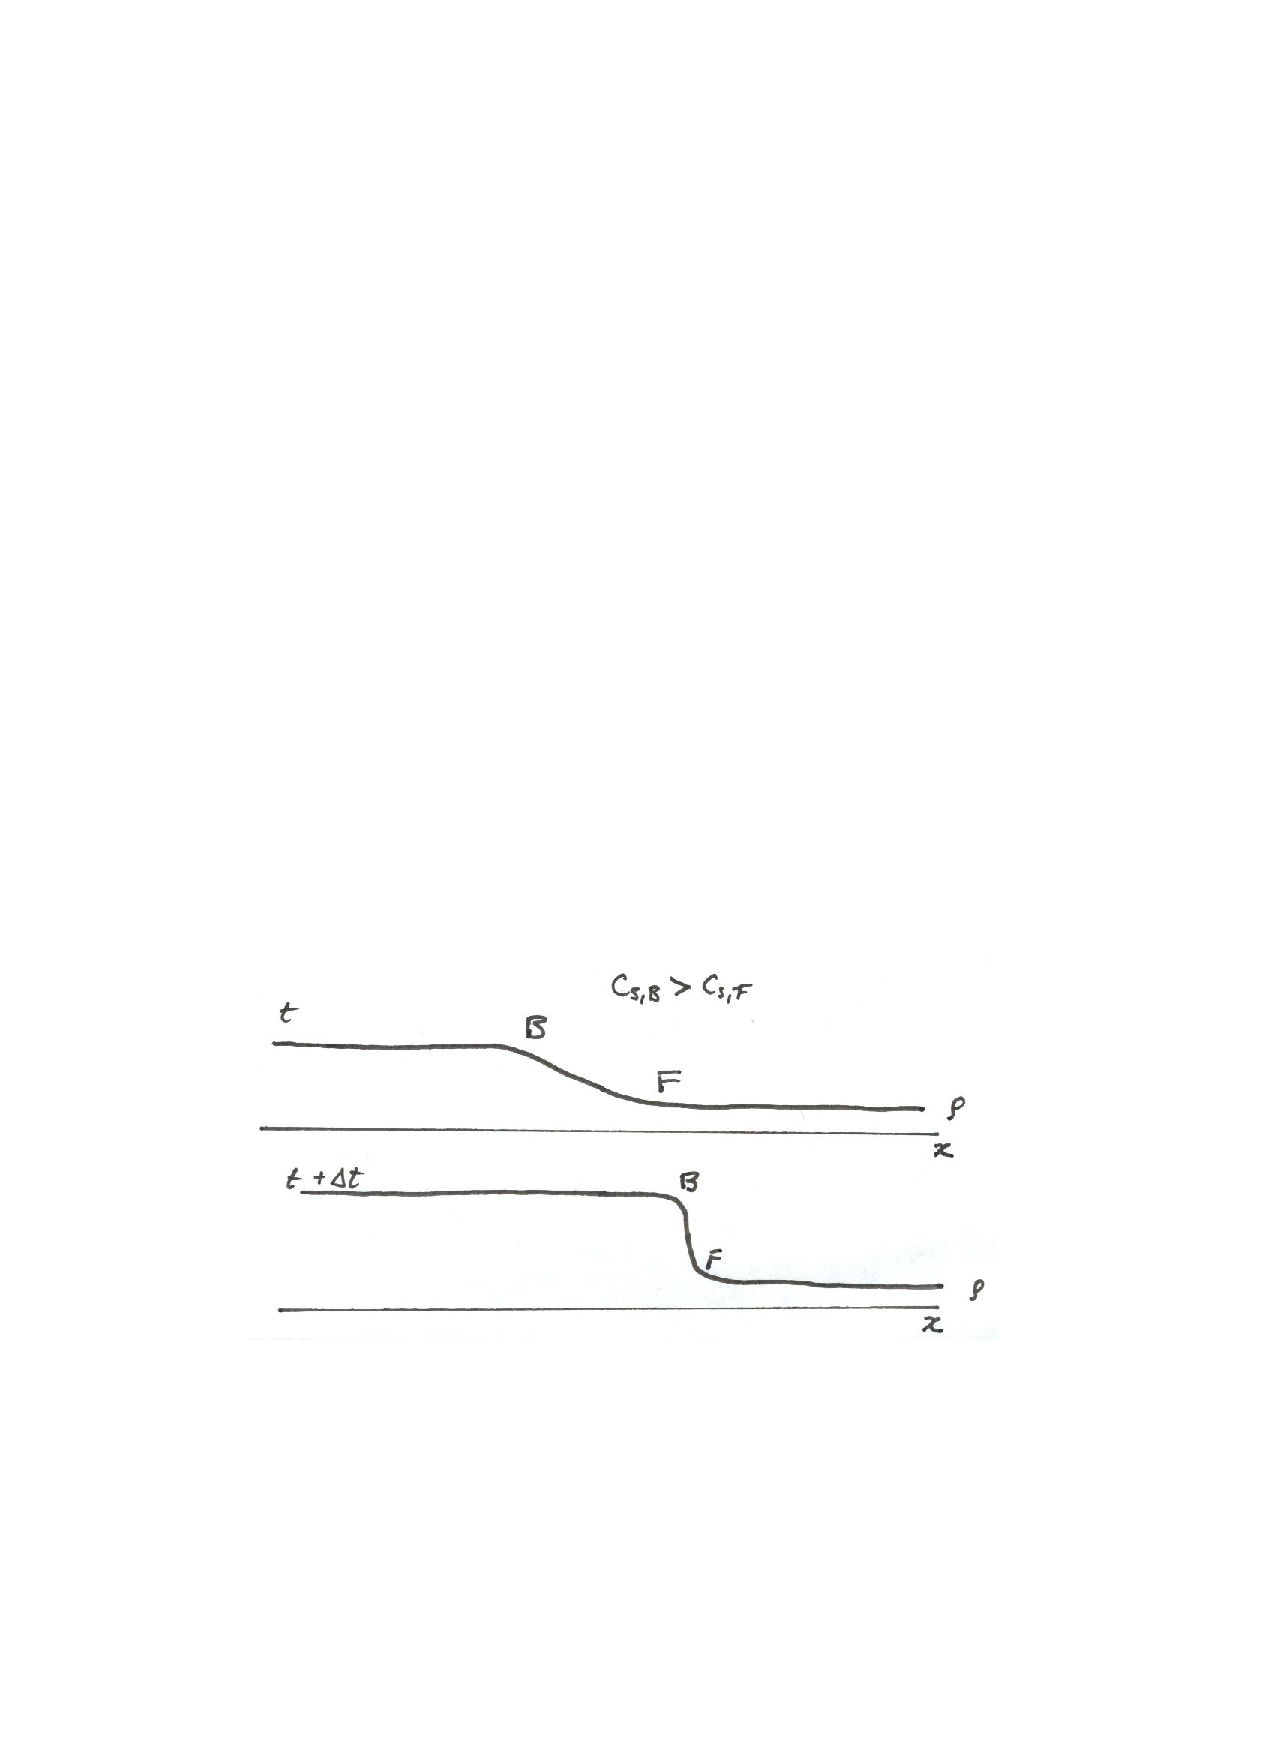
\includegraphics[width=\textwidth]{shock-formation}
\caption{Schematic of a disturbance steepening as it propagates.  The plots show the density $\rho$ at time $t$ (\emph{top panel}) and a time $\Delta t$ later (\emph{bottom panel}) for a disturbance propagating along the $x$-direction.  Because the sound speed is greater in the compressed region, the ``back'' of the disturbance $B$ moves faster than the front $F$: as a result, the disturbance steepens. }
\label{f.steepening}
\end{figure}

To illustrate the properties of a shock, we'll use our thought experiment of a piston being pushed into a tube filled with gas, as illustrated in Fig.~\ref{f.piston}.  The piston moves to the right with velocity $u$.  We assume that the piston has been pushing the fluid for a while at constant velocity, so that any transients have died down, leaving a simple flow structure at $t=0$ (Fig.~\ref{f.piston}, \emph{top panel}): far from the piston, the fluid is at rest, with density $\rho_{0}$, pressure $p_{0}$, and internal energy $\varepsilon_{0}$; a shock propagates into this fluid with velocity $D$; between the shock and the piston the fluid moves with the same velocity, $u$, as the piston and has density $\rho_{1}$, pressure $p_{1}$, and $\varepsilon_{1}$.

\begin{figure}[htbp]
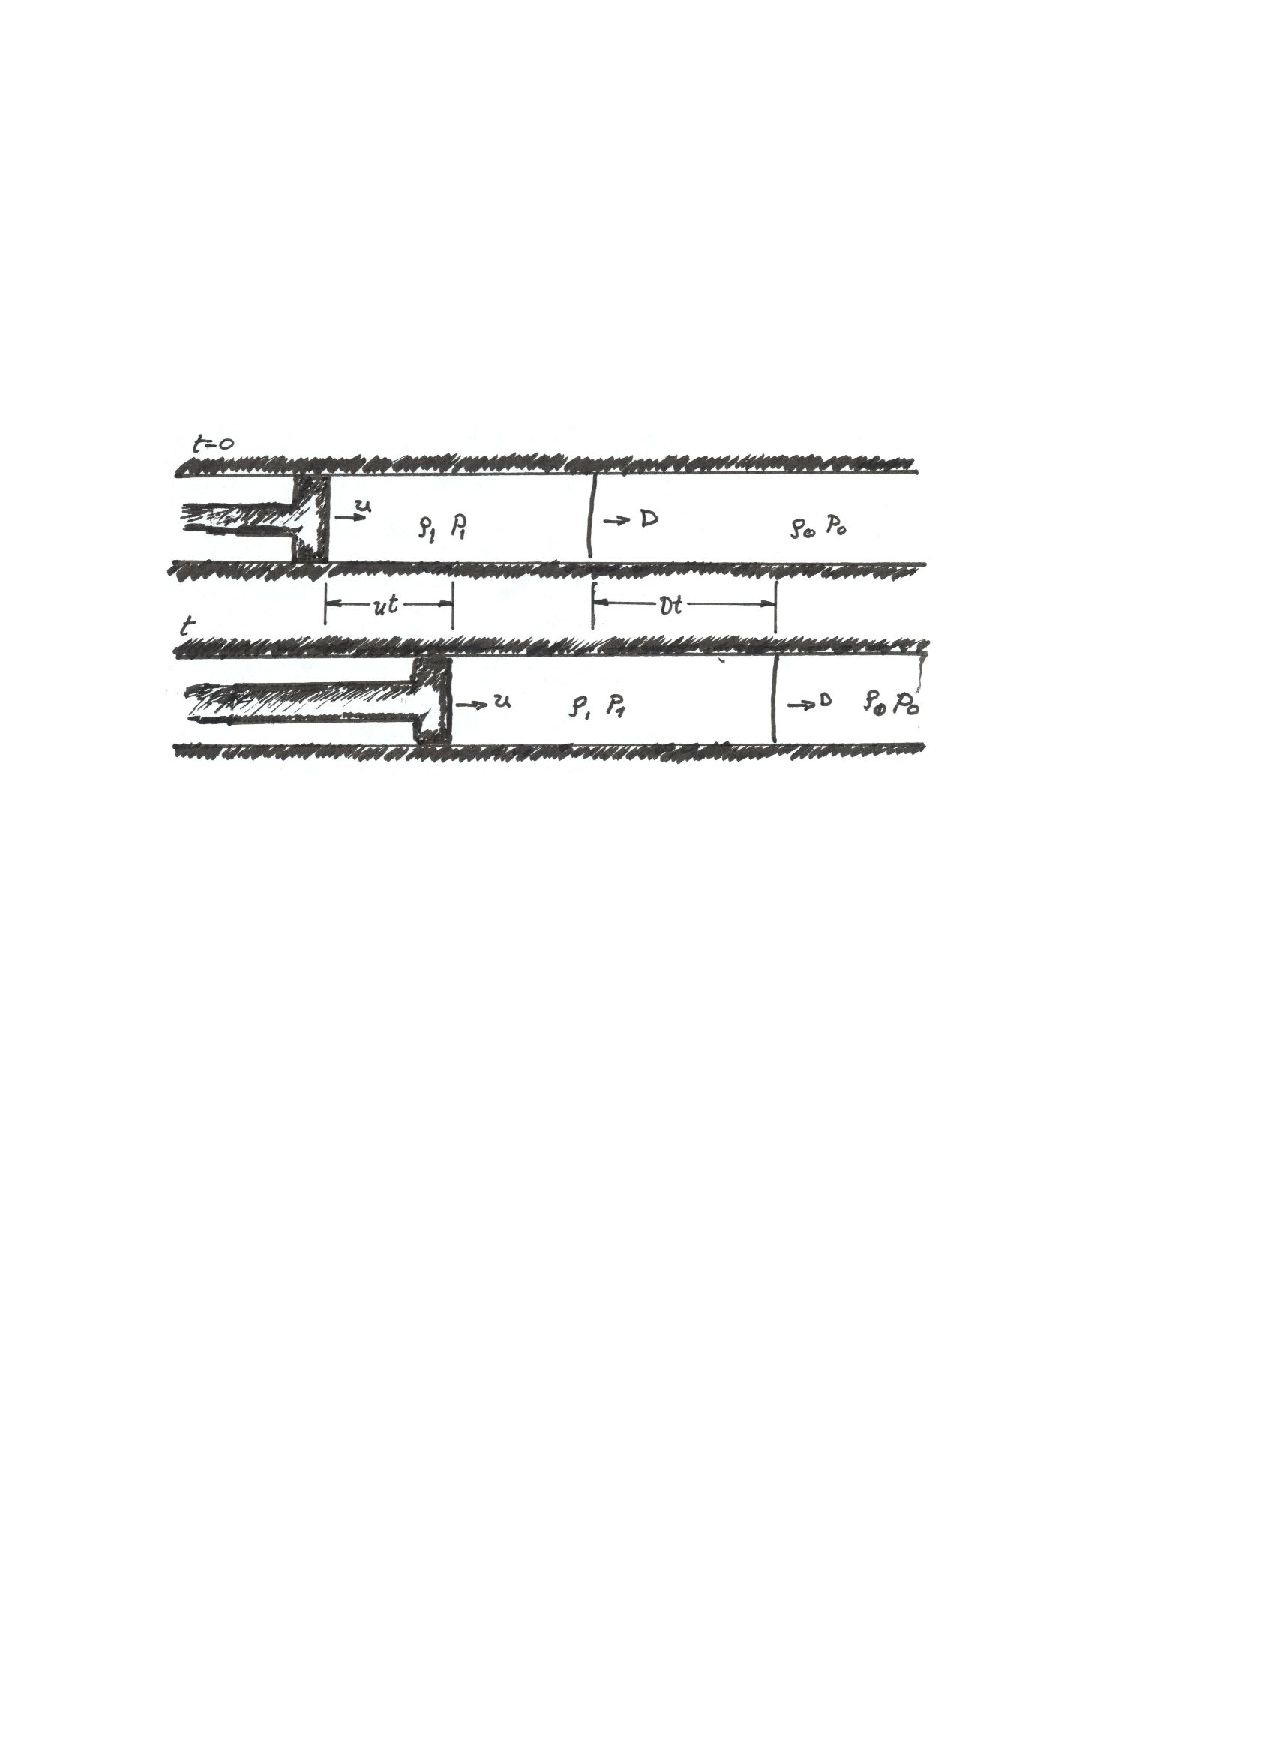
\includegraphics[width=\textwidth]{piston}
\caption{Schematic of a piston driving a shock.  In this schematic, the shock propagates at velocity $D$.}
\label{f.piston}
\end{figure}

In a time $t$, the piston has moved (Fig.~\ref{f.piston}, \emph{botton panel}) a distance $ut$, and the shock has moved a distance $Dt$; the mass of the ``shocked'' fluid has therefore increased by $\rho_{1}(D-u)t$.  This must equal the mass swept up by the shock, namely $\rho_{0}Dt$.  We therefore have our first relation,
\begin{equation}\label{e.shock-mass-1}
\rho_{1}(D-u) = \rho_{0}D.
\end{equation}
The fluid swept up by the shock now has velocity $u$ and thus a momentum $(\rho_{0}Dt)u$. This increase in momentum must equal the net impulse imparted to the fluid, $(p_{1}-p_{0})t$.  We therefore have our second relation,
\begin{equation}\label{e.shock-momentum-1}
p_{1} - p_{0} = D\rho_{0}u.
\end{equation}
The fluid swept up by the shock has a change in total energy, $(\rho_{0}D t)(\varepsilon_{1} + u^{2}/2 -\varepsilon_{0})$. This must equal the work done on the fluid by the piston, which is the force times displacement $p_{1}ut$.  We therefore have our third relation,
\begin{equation}\label{e.shock-energy-1}
\rho_{0}D\left[\varepsilon_{1}-\varepsilon_{0} + \frac{1}{2}u^{2}\right] = p_{1}u.
\end{equation}
To abstract the problem, we transform to a frame moving with the shock.  In this frame the upstream velocity ahead of the shock has velocity $u_{0} = -D$; the downstream velocity is $u_{1} = u-D$.  The difference in velocity is $|u_{0} - u_{1}| = u$.
In this frame, equations~(\ref{e.shock-mass-1}), (\ref{e.shock-momentum-1}), and (\ref{e.shock-energy-1}) take on the more familiar forms,
\begin{eqnarray}
\rho_{1}u_{1} &=& \rho_{0}u_{0},\label{e.shock-mass-2}\\
p_{1} + \rho_{1}u_{1}^{2} &=& p_{0} + \rho_{0}u_{0}^{2},\label{e.shock-momentum-2}\\
(\rho_{1}u_{1})\left[\varepsilon_{1} + \frac{1}{2}u_{1}^{2} + \frac{p_{1}}{\rho_{1}}\right] &=& 
	(\rho_{0}u_{0})\left[\varepsilon_{0} + \frac{1}{2}u_{0}^{2} + \frac{p_{0}}{\rho_{0}}\right]. 
			\label{e.shock-energy-2}
\end{eqnarray}
Recognize these?  Compare with equations~(\ref{e.mass-1}), (\ref{e.momentum-2}), and (\ref{e.energy-2}), and recognize that equations~(\ref{e.shock-mass-2}), (\ref{e.shock-momentum-2}), (\ref{e.shock-energy-2}) just express that the downstream mass flux, momentum flux, and energy flux equal their upstream counterparts.

Equations~(\ref{e.shock-mass-2}), (\ref{e.shock-momentum-2}), (\ref{e.shock-energy-2}), when supplemented with an equation of state, are sufficient to allow solution for $p_{1}$ and $\rho_{1}$ in terms of $p_{0}$, $\rho_{0}$ and $u$. To explore the properties of the shock, we adopt a simple ideal adiabatic equation of state: $p =  (\gamma - 1)\rho\varepsilon = K \rho^{\gamma}$ with sound speed $c^{2} = \gamma p/\rho$.  The enthalpy is then
\[ \varepsilon + \frac{p}{\rho} = \frac{\gamma}{\gamma-1}\frac{p}{\rho}. \]
Using this equation of state, we can reduce equations~(\ref{e.shock-mass-2}), (\ref{e.shock-momentum-2}), (\ref{e.shock-energy-2}) into expressions in terms of the pressure ratio $P = p_{1}/p_{0}$:
\begin{eqnarray}
	\textrm{density ratio,}&\qquad& \frac{\rho_{1}}{\rho_{0}} 
			= \frac{\gpo P + \gmo}{\gmo P +  \gpo};\\
	\textrm{entropy increase,} &\qquad& s_{1}-s_{0} 
		= c_{v}\ln\left[\frac{p_{1}}{p_{0}}\left(\frac{\rho_{0}}{\rho_{1}}\right)^{\gamma}\right];\\
	\textrm{temperature ratio,} &\qquad& \frac{T_{1}}{T_{0}} = \frac{p_{1}}{p_{0}}\frac{\rho_{0}}{\rho_{1}};\\
	\textrm{upstream Mach,} &\qquad& \left(\frac{u_{0}}{c_{0}}\right)^{2} = \frac{\gpo P + \gmo}{2\gamma};\\
	\textrm{downstream Mach,} &\qquad& \left(\frac{u_{1}}{c_{1}}\right)^{2} 
			= \frac{\gmo P + \gpo}{2\gamma P}.
\end{eqnarray}
In the limiting case of a strong shock, $P \gg 1$, the density increase is finite: $\rho_{1}/\rho_{0} \to \gpo/\gmo$; for $\gamma = 5/3$, $\rho_{1}/\rho_{0}\to 4$.  The temperature and entropy jumps across the shock, however, scale with $P$ and are arbitrarily large.  The upstream Mach number is likewise proportional to the pressure ratio, $\Ma_{0}^{2} \to \gpo P/(2\gamma)$, but the downstream flow is subsonic, $\Ma_{1}^{2} \to \gmo/(2\gamma)$. The shock transforms the ordered (low-entropy) supersonic upstream flow into the disordered (high-entropy) subsonic downstream flow.


\end{document}
